%% 
%% Copyright 2007-2020 Elsevier Ltd
%% 
%% This file is part of the 'Elsarticle Bundle'.
%% ---------------------------------------------
%% 
%% It may be distributed under the conditions of the LaTeX Project Public
%% License, either version 1.2 of this license or (at your option) any
%% later version.  The latest version of this license is in
%%    http://www.latex-project.org/lppl.txt
%% and version 1.2 or later is part of all distributions of LaTeX
%% version 1999/12/01 or later.
%% 
%% The list of all files belonging to the 'Elsarticle Bundle' is
%% given in the file `manifest.txt'.
%% 
%% Template article for Elsevier's document class `elsarticle'
%% with harvard style bibliographic references

\documentclass[preprint,12pt]{elsarticle}

%% Use the option review to obtain double line spacing
%% \documentclass[preprint,review,12pt]{elsarticle}

%% Use the options 1p,twocolumn; 3p; 3p,twocolumn; 5p; or 5p,twocolumn
%% for a journal layout:
%%\documentclass[final,1p,times]{elsarticle}
%% \documentclass[final,1p,times,twocolumn]{elsarticle}
%% \documentclass[final,3p,times]{elsarticle}
%% \documentclass[final,3p,times,twocolumn]{elsarticle}
%%\documentclass[final,5p,times]{elsarticle}
%% \documentclass[final,5p,times,twocolumn]{elsarticle}

%% For including figures, graphicx.sty has been loaded in
%% elsarticle.cls. If you prefer to use the old commands
%% please give \usepackage{epsfig}

%% The amssymb package provides various useful mathematical symbols
\usepackage{amssymb}
%% The amsthm package provides extended theorem environments
\usepackage{amsthm}
\usepackage{amsmath}
\usepackage{amsfonts}
\usepackage{amssymb}
\usepackage{array}
\usepackage{subfig}
\usepackage{booktabs}
\usepackage{multirow}
\usepackage{geometry}
\geometry{left=2.5cm, right=2.5cm, top=2.5cm, bottom=2.5cm}

\newcommand{\kwh}{kW$\cdot$h}
%% The lineno packages adds line numbers. Start line numbering with
%% \begin{linenumbers}, end it with \end{linenumbers}. Or switch it on
%% for the whole article with \linenumbers.
%% \usepackage{lineno}

\journal{Applied Energy}

\begin{document}

\begin{frontmatter}

%% Title, authors and addresses

%% use the tnoteref command within \title for footnotes;
%% use the tnotetext command for theassociated footnote;
%% use the fnref command within \author or \address for footnotes;
%% use the fntext command for theassociated footnote;
%% use the corref command within \author for corresponding author footnotes;
%% use the cortext command for theassociated footnote;
%% use the ead command for the email address,
%% and the form \ead[url] for the home page:
%% \title{Title\tnoteref{label1}}
%% \tnotetext[label1]{}
%% \author{Name\corref{cor1}\fnref{label2}}
%% \ead{email address}
%% \ead[url]{home page}
%% \fntext[label2]{}
%% \cortext[cor1]{}
%% \affiliation{organization={},
%%             addressline={},
%%             city={},
%%             postcode={},
%%             state={},
%%             country={}}
%% \fntext[label3]{}

\title{Dual-Centralized Control Scheme and FF-DHRL-based Collaborative Optimization for Charging Stations under Intra-Day Peak-Shaving Demand}

%% use optional labels to link authors explicitly to addresses:
%% \author[label1,label2]{}
%% \affiliation[label1]{organization={},
%%             addressline={},
%%             city={},
%%             postcode={},
%%             state={},
%%             country={}}
%%
%% \affiliation[label2]{organization={},
%%             addressline={},
%%             city={},
%%             postcode={},
%%             state={},
%%             country={}}

% \author{}

% \affiliation{organization={},%Department and Organization
%             addressline={}, 
%             city={},
%             postcode={}, 
%             state={},
%             country={}}
%%
\author[1,2]{Fang Daohong}
\ead{fangdaohong@mail.hfut.edu.cn}

\author[1]{Tang Hao \corref{cor1}}
\ead{htang@hfut.edu.cn}

\author[1]{Zhang Tao}  
\ead{zhangtao@hfut.edu.cn}

\author[1]{Zhang Qianli}  
\ead{qianli_z@163.com}

\address[1]{School of Electrical Engineering and Automation, Hefei University of Technology, Hefei, 230009, China}
\address[2]{School of Electrical and Computer Engineering, National Technical University of Athens, Athens, 10682, Greece}

\cortext[cor1]{Corresponding author}

%%

\begin{abstract}
%% Text of abstract
% The rising popularity of electric vehicles (EVs) offers considerable opportunities for charging stations to support the peak demands of power grid (PG). These stations indirectly affect hourly electricity consumption by varying service prices and adjust charging power in real time following peak-shaving directives. Nevertheless, the unpredictable EV flow and the immediacy of real-time peak-shaving commands pose substantial challenges make this a challenging and multifaceted issue. To tackle this, we model EV charging behavior as a non-homogeneous Poisson process within a framework based on queuing theory and charging pile capacity constraints. We establish a dual-centralized control scheme comprising a Service Price Maker (SPM) and a Charging Power Controller (CPC), and apply Deep Hierarchical Reinforcement Learning (DHRL) to achieve stochastic optimization targets.  The SPM operates at the upper layer to maximize economic benefits, while the CPC at the lower layer aims to balance peak-shaving benefits with EV user satisfaction. This method proactively  manages service prices and charging powers in response to dynamic electricity prices and real-time peak-shaving commands from PG. Moreover, Feature Fusion (FF) technology is utilized to streamline high-dimensional data into critical low-dimensional inputs within the input layer of deep network. Ultimately, our collaborative FF-DHRL optimization approach, empirically tested, fulfills the station's comprehensive goals while meeting intra-day peak-shaving demands. 基于采用价格间接引导和实时功率控制两种调节方式,充电场站可以在日内以响应电网电价和实时调峰指令。同时,我们将women1
The growing use of electric vehicles (EVs) enhances charging stations' role in balancing power grid demands via dynamically pricing and adjusting charging power adjustment strategies. However, the unpredictable EV flow and the immediacy of real-time peak shaving present complex challenges. This paper introduces a novel dual-centralized control scheme and a learning optimization method. It adopts a station operation model based on queueing theory, considering charging pile capacity constraints. The proposed control scheme, integrating a Service Price Maker (SPM) and Charging Power Controller (CPC), adapts service prices and charging power in response to electricity prices and peak-shaving directives. Employing a model-free Deep Hierarchical Reinforcement Learning (DHRL) approach, the SPM targets economic maximization, while the CPC aims to balance peak-shaving efficacy and user satisfaction.  Furthermore, to improve the offline learning efficiency of the algorithm, feature fusion (FF) technology is used to condense high-dimensional data into essential low-dimensional features, improving the algorithm's learning efficiency.The effectiveness of the proposed FF-DHRL was verified in a simulated charging station system.
\end{abstract}

%%Graphical abstract
\begin{graphicalabstract}
%\includegraphics{grabs}
\end{graphicalabstract}

%%Research highlights
\begin{highlights}
\item Research highlight 1
\item Research highlight 2
\end{highlights}

\begin{keyword}
%% keywords here, in the form: keyword \sep keyword
EV charging station management \sep Queuing theory\sep Deep hierarchical reinforcement learning\sep Demand response\sep  Feature fusion.
%% PACS codes here, in the form: \PACS code \sep code

%% MSC codes here, in the form: \MSC code \sep code
%% or \MSC[2008] code \sep code (2000 is the default)
\end{keyword}

\end{frontmatter}

%% \linenumbers

%% main text
\section{Introduction}
\label{}
The increasing focus on reducing energy consumption and environmental impact underscores the critical role of new-energy vehicles, particularly EVs, in shaping the future energy landscape. Nonetheless, integrating EVs into the power grid, especially in an unregulated manner, presents
challenges\citep{wang_coordinated_2023}. Uncoordinated charging patterns
may exacerbate peak load issues in the power grid, exemplified by
the "adding peak to peak" phenomenon, potentially overloading local distribution networks. Conversely, when EV charging is effectively managed, it offers substantial benefits
to the grid, thanks to the inherent flexibility of EV charging systems. \citet{gao_combined_2023} and another study \citet{2020FrequencyReserve} have investigated the scheduling of EV charging and discharging to aid in real-time and day-ahead frequency regulation of the grid. \citet{chen_Ancillary_Service} developed an autonomous energy management strategy for photovoltaic-assisted power stations, enabling charging stations to contribute to ancillary services of the smart grid. Further, \citet{wang_optimal_2020} demonstrated how integrating EV charging stations with energy storage and renewable energy generation can form a micro-grid, thereby enhancing the integration of renewable energy sources through strategic management of charging and discharging schedules.

The management and coordination of  EVs in the grid, often require diverse strategies to enhance user participation and response. Among these, demand response (DR) mechanisms have emerged
as a prevalent choice, as noted by \citet{Mohandes_Demand_Response}. DR strategies can be categorized into two types: price-based and incentive-based, depending on whether the electricity price directly serves as the guiding signal for response \citep{FANShuai2022}. Common price-based
DR approaches include peak-to-valley tariffs and dynamic real-time tariffs. \citet{lin_minimizing_2022} focused on minimizing operation costs of EVs' charging under real-time pricing from the power grid and developed online algorithms to balance charging
costs with user satisfaction. On the other hand, incentive-based DR encompasses methods like direct load control and orderly power management during peak or valley periods. \citet{fang_aggregator-based_2020} introduced an aggregator-based demand response mechanism for EVs, aimed at peak regulation during off-peak hours, addressing the challenges faced by power grids with limited peak regulation capacity. Consequently, regardless of the approach, be it price-based or incentive-based,
EV charging stations play a pivotal role in mitigating supply-demand imbalances in the grid.

From the perspective of EV charging stations, responding to grid demands
involves two control modes: direct and indirect control. Indirect
control enables EV aggregators to subtly influence customer charging
behavior through pricing signals or incentives. \citet{2021A} developed a bi-level optimization model based on the Stackelberg game theory, adjusting charging prices dynamically to induce load shifting in consumer charging behaviors. This indirect mode, characterized by its simplicity and suitability for day-ahead or intra-day hourly load management, lacks flexibility for real-time power regulation. In contrast, direct control entails EV aggregators
actively managing the charging powers of EVs during periods requiring
load adjustment, in line with higher-level dispatch directives. This
mode offers rapid load adjustment and high precision, but may compromise
user satisfaction due to potential power shortages \citep{2017Real}.
Our approach seeks to amalgamate the strengths of both modes: initially,
we adjust the power consumption of charging stations using service
price adjustments at a broader time scale, followed by minute-level
power control for real-time dispatch responses. This cooperative approach
of service pricing and power control enables load adjustment at various
intraday timescales, aiming to enhance economic returns and peak regulation
effectiveness. Current research on intraday peak-shaving response
strategies for EV charging stations has yet to explore this integrated
control framework extensively.

Numerous scholars have delved into optimizing charging service strategies
for EV charging stations. \citet{yan_optimized_2019}
segmented the scheduling problem of integrated charging stations with
photovoltaic (PV) systems and battery storage into four stages and
used direct control approach for intra-day scheduling. This division
accounts for uncertainties in PV generation, charging demands, and
grid power supply, with a detailed strategy-solving process for each
stage. \citet{yuan_scheduling_2022} proposed a
polynomial-time online optimization method based on an indirect control
approach for auction mechanism. This method incentivizes charging
stations to utilize their local generators for energy production and
participate in emergency demand response. These studies typically
conceptualize the EV charging service issue as a model-based control
problem, and such model-based methodologies have shown considerable
effectiveness in EV charging scheduling for their respective target
systems. Nevertheless, the incorporation of uncertainties in EV user
charging behavior and the need for real-time response present significant
challenges to these model-based approaches.

Recent advancements in model-free approaches, which operate without
requiring specific system model information, have shown considerable
success in decision-making applications. This progress has inspired
significant achievements in EV charging control strategies and smart
grid applications using model-free methods. \citet{di_research_2022,zhang_optimization_2022}
established multi-objective EV load scheduling optimization models
and employed particle swarm optimization (PSO) algorithms to optimize
charging scheduling strategies, achieving orderly charging of EV fleets.
However, PSO is only suitable for single-section problems and not
for continuous sectional decision optimization generally. Reinforcement
learning (RL) performs well in continuous sectional optimization problems.
\citet{2015Optimal}'s study explored a fully automated
energy management system that uses a Q-table based on data learning
for decision-making, optimizing system efficiency through smart device
switching. However, our preliminary research \citep{tang_access_2022}
found that in large systems with multiple decision state dimensions,
such as optimal scheduling of charging stations, Q-learning may encounter
a dimensionality explosion problem. \citet{wan_model-free_2019}
proposed a deep RL algorithm DQN combined with a Long Short-Term Memory
(LSTM) network structure, inputting information such as charging prices
into the deep network in a time-series manner, combining the perception
capability of deep networks with the optimization ability of reinforcement
learning to form a real-time EV charging strategy. Deep networks enable
us to consider more system states, such as service price, real-time
charging power, SoC, and queue length. Theoretically, this can improve
strategy performance, but in practice, the increase in state dimensions
and information volume may lead to sparser data distributions and
more complex relationships, thereby impacting optimization outcomes.\citep{DBLP:journals/joeuc/Yu22}

% In this study, we developed a cooperative control scheme integrating
% service price regulation and real-time charging power control. This
% scheme leads to a bi-layer sequential decision-making process, taking
% into account the stochastic nature of EV flow and intra-day peak-shaving
% demands. We introduced a model-free collaborative optimization approach
% based on DHRL to address these challenges. Furthermore, to mitigate
% information redundancy at the input layer, we implemented a FF method,
% which effectively condenses high-dimensional decision data into key
% features, thereby increasing the algorithm's learning efficiency.
% The contributions of this study are summarized as follows:

Motivated by the aforementioned facts, this paper proposes a new dual-centralized control scheme and FF-DHRL based collaborative optimization method for peak shaving response in charging stations. The main contributions of the paper are summarized as follows:

\begin{itemize}
\item A dual-centralized control scheme integrating service price maker and real-time charging power controller is proposed. In this scheme, the SPM modulates the service price in response to grid electricity prices, influencing EV charging behavior and facilitating hourly adjustments
to the station's electricity load. Concurrently, when the higher-level
dispatch center issues real-time peak-shaving commands, the CPC dynamically
adjusts the charging powers based on these commands and the station's
operational status.This cooperative scheme allows the station
to efficiently meet the grid's demand response needs during operation.
\item A model-free hierarchical cooperative optimization method based on DHRL is developed, and enhanced through FF technology. In this method, the SPM as the upper layer focuses on maximizing economic profits, while the CPC at the lower layer strives to balance peak shaving benefits and user satisfaction. Through DHRL, using interaction data between agents and the simulation environment for training, the desired objectives are achieved under the randomness of EV mobility and real-time peak-shaving commands. Additionally, by employing FF technology, low-dimensional, fused features are generated and applied directly to charging service pricing. This approach not only effectively compresses the state space of the upper-level agent but also retains the agent's perceptual ability and enhances learning efficiency.
% \item We developed a bi-layer sequential decision-making process driven
% by time-events, using DHRL for strategy optimization. The SPM, as
% the upper layer, focuses on maximizing economic gains, while the CPC,
% as the lower layer, aims to balance peak-shaving revenue and user
% satisfaction. EV arrivals follow non-homogeneous Poisson processes,
% with grid price cycles and random peak-shaving orders driving the
% upper and lower layer decisions respectively. Through DHRL, utilizing
% the interaction data between agents and the simulation environment
% for training, we achieve the maximization of the desired objectives
% under the randomness of EV mobility and real-time peak-shaving orders.
% \item We have designed an early feature fusion layer to efficiently extract
% crucial decision features from the original state of the upper layer.
% By employing this method, we produce low-dimensional, fused features
% that are directly applied to charging service pricing, effectively
% minimizing the state space of the upper agent. This strategic reduction
% not only retains the agent's perceptual capabilities but also simplifies
% the algorithm's complexity and bolsters its learning efficiency.
\end{itemize}

The rest of the paper is organized as follows: Section II introduces
the problem formulation. Section III elaborates on our approach, utilizing
deep hierarchical reinforcement learning, and details improvements
made to the algorithm. In Section IV, we present a series of experiments
to validate the efficacy of our proposed method. Finally, Section
V gives a conclusion.


\section{Problem Formulation}
%%\label{}
In this section, we analyze commercial charging stations, which generate revenue by providing charging services to EV users and simultaneously contribute to grid stability by responding to peak-shaving demands. Initially, we establish an operation model for these stations based on queueing theory, accounting for the stochastic nature of EV arrivals and the finite capacity of charging piles and queues. Subsequently, we develop demand response mechanisms inspired by practices in Anhui Province, China, incorporating price-based strategies and real-time peak regulation. Our cooperative control scheme for the EV charging station integrates two key components: the Service Price Maker (SPM) and the Charging Power Controller (CPC), as illustrated in Fig. \ref{fig:The-system-architecture}. These units independently manage service pricing and charging power, respectively, while synergistically working to optimize the station's overall efficiency.
\begin{figure}[tbh]
    \centering
    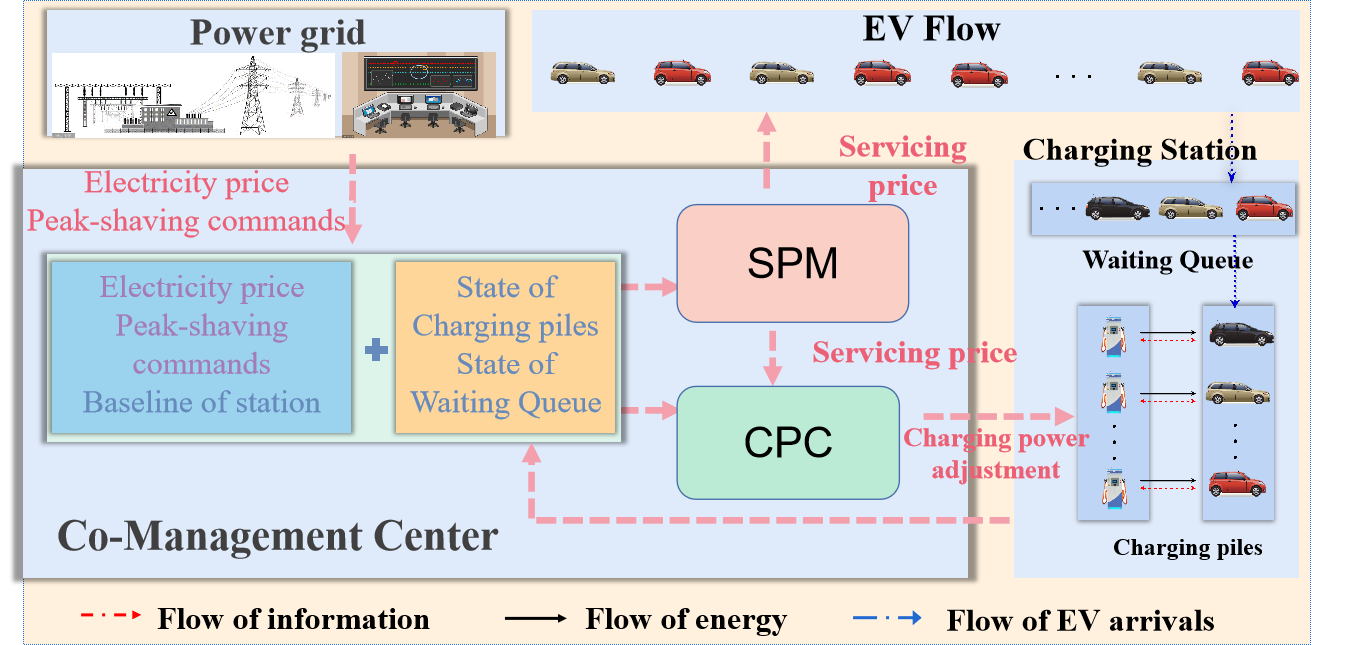
\includegraphics[width=1\linewidth]{figures/operating_mode.png}
    \caption{The system architecture of fast charging station}
    \label{fig:The-system-architecture}
\end{figure}

\subsection{Operation Mode of Charging Stations}
The charging station is equipped with $J$ DC fast charging piles
and waiting queue. Each charging pile in the station could meet the
charging demands of $M$ types of fast charging EVs and change the
charging power according to the commands of the CPC. The $J$ charging
piles are denoted as $cs_{1},cs_{2},\ldots,cs_{J}$, respectively.
At moment $t$, the state of the charging pile $cs_{j}(t)$ is represented
as
\begin{equation}
c_{j}(t)=\{m_{j},H_{m_{j}}(t),E_{m_{j}},P_{m_{j}}^{max},p_{j}(t),I_{m_{j}}\},j\in[1,J]\label{eq:cjt}
\end{equation}
where $m_{j}$,$E_{m_{j}}$ and $P_{m_{j}}^{max}$ are the type, battery
capacity and rated charging power of the EV on the charging pile $cs_{j}$,
respectively; $H_{m_{j}}(t)$ and $p_{j}(t)$ are represent real-time
SoC and charging power of this EV at time $t$, respectively; $I_{m_{j}}$
is time of EV connection to the charging pile. If the charging pile
$cs_{j}$ was idle, then $c_{j}(t)=\{0,0,0,0,0,0\}$. 
In this study, we primarily consider the constant power charging phase of EV charging.
Therefore, their state of charge $H_{m_{j}}(t)$ occur as a function of charging time with the charging efficiency being $\eta$, following Eq. \ref{eq:EV_soc_tran}. 
\begin{equation}
H_{m_{j}}(t)=H_{m_{j}}(I_{m_{j}})+\eta\int_{I_{m_{j}}}^{t}p_{j}(\omega)d\omega/E_{m_{j}}\label{eq:EV_soc_tran}
\end{equation}

In further, we define the joint state of $J$ charging piles at time $t$ as follows:
\[
C(t)=\{c_{1}(t),c_{2}(t),\ldots,c_{j}(t),\ldots,c_{J}(t)\}.
\]

The waiting queue consists of waiting spaces where newly arrived EV
wait when there is no vacant charging pile. Without loss of generality,
assume that the maximum number of waiting EVs is $L$ and that there
is no loss of EV users during the queueing process. Therefore, the
$L$ waiting spaces are recorded as $W_{1},W_{2},\ldots,W_{L}$, respectively.
The state of $l$th waiting space at time $t$ is denoted as
\begin{equation}
\begin{array}{c}
w_{l}(t)=\{\widetilde{m}_{l}(t),H_{\widetilde{m}_{l}}(t),E_{\widetilde{m}_{l}}(t),P_{\widetilde{m}_{l}}^{max}(t)\}\\
l\in\Phi_{L}=\{1,2,\ldots,L\}
\end{array}\label{eq:wlt}
\end{equation}
where $\widetilde{m}_{l}(t)$ and $H_{\widetilde{m}_{l}}(t)$ are
the type and SoC of the EV on the waiting space $W_{l}$, respectively;
$E_{\widetilde{m}_{l}}(t)$ and $P_{\widetilde{m}_{l}}^{max}(t)$
are battery capacity and rated charging power of this EV. Then let
$l_{rear}(t)$ be the number of EVs in the waiting queue at time $t$,
the state of the waiting queue is as follows:
\begin{equation}
W(t)=\{w_{1}(t),w_{2}(t),\ldots,w_{l}(t),\ldots,w_{L}(t)\}.\label{eq:wt}
\end{equation}

And if the waiting queue is not completely full, that is $l_{rear}(t)<L$,
which for any integer $l$ in the interval $(l_{rear}(t),L]$, $w_{l}(t)=\{0,0,0,0\}$.

Combining the characteristics of the actual EV flow, we take it that
the EVs of the service system arrive at the charging station randomly
to request charging service. Considering the independence of the EV
arrival events, the EV flow has assumed to follow a non-homogeneous
Poisson process with the arrival rate $\lambda(t)$. 
% and we assumed
% that each type of EV arrived independently with arrival rate \(\lambda_{m}(t),m\in\phi_{M}=\{1,2,\cdots,M\}\). Accordingly, $\lambda(t)=\sum_{m=1}^{M}\lambda_{m}(t)$, and the probability of the arrival EV being type m is $\lambda_{m}(t)/\lambda(t)$.

If an EV arrives at the charging station at time $t$ for charging
service, and we define the event as $e_{t}=\{m_{0}(t),H_{m_{0}}(t)\}$, where $m_{0}(t)\in\phi_{M}=\{1,2,\cdots,M\}$
is the type of arriving EV and $H_{m_{0}}(t)$ is its SoC. As $e_{t}$
occurs,the state of the charging station will change according to
the following three conditions. The first condition is that waiting
queue and charging piles are full, i.e. $c_{j}(t)\neq0$ for any $j\in [1,J]$
and $l_{rear}(t)=L$, this EV leaves the station immediately. The
state of the charging station will not change at this time. The second
condition is that the waiting queue has free spaces and is not completely
empty, i.e. $1\leq l_{rear}(t)<L$ and $c_{j}(t)\neq0$ for any $j$
in $\phi_{J}$, the arrival enters the waiting space $W_{l_{rear}+1}$,
meanwhile, the state of waiting space $W_{l_{rear}+1}$ changes accordingly
as in Eq. \ref{eq:w_change}.
\begin{equation}
\begin{array}{c}
w_{l_{rear}+1}(t^{+})=\{m_{0}(t),H_{m_{0}}(t),E_{m_{0}},P^{max}_{m_{0}}\}\\
l_{rear}(t^{+})= l_{rear}(t)+1
\end{array}\label{eq:w_change}
\end{equation}

The last condition is when there is an idle charging pile, the arrival is randomly connected to an idle charging pile $cs_{j}$ with initial charging power $\overline{p}$, meanwhile, the state of this charging pile changes accordingly as in Eq. \ref{eq:cj_change}.

\begin{equation}
c_{j}(t^{+})=\{m_{0}(t),H_{m_{0}}(t),E_{m_{0}},P_{m_{0}}^{max},\bar{p},t\}\label{eq:cj_change}
\end{equation}

Generally, EVs immediately leave the charging station upon their SoC reaching the common charging target $\tilde{H}$. If an EV is waiting and a vehicle leaves the station, the waiting EVs connect to any idle charging pile $cs_{j}$ based on the FIFO (first-in, first-out) principle. Accordingly, the process of state changes for the charging piles and the waiting queue is shown in Eq. \ref{eq:EV_in_pile}. The first step is to connect the EV in the first waiting space $W_{1}$ to any idle charging pile $cs_{j}$ with an initial charging power $\bar{p}$, and the state of this EV, included its type $\tilde{m}_{1}(t)$ and SoC $H_{\tilde{m}_{1}}(t)$, is assigned to $c_{j}(t)$. At the meantime, the EVs in the queue in turn to pass forward a waiting space.

\begin{equation}
\begin{array}{c}
c_{j}(t^{+})=\{\tilde{m}_{1}(t),H_{\tilde{m}_{1}}(t),E_{\tilde{m}_{1}},P_{\tilde{m}_{1}}^{max},\bar{p},t\}\\
w_{l}(t^{+})=w_{l+1}(t),1\leq l<l_{rear}(t)\\
w_{l_{rear}}(t^{+})=\{0,0,0\}\\
l_{rear}(t^{+})=l_{rear}(t)-1
\end{array}\label{eq:EV_in_pile}
\end{equation}
\subsection{DR mechanisms and Dual-Centralized Control Scheme}
In this subsection, we focus on the cooperative control scheme of the charging station under demand response mechanisms which contain the price-base and incentive-based. During operation, charging stations need to consider not only economic benefits but also their response to grid load management. Charging stations, as a flexible resource load, on one hand, it can manage the charging behavior of EVs by adjusting the service prices based on the grid's TOU electricity tariff. On the other hand, during emergency periods, charging stations can respond to real-time peak shaving commands from the grid by adjusting the station's charger power, alleviating load pressure. Thus, a dynamic electricity tariff and real-time peak shaving mechanisms for the EV charging station are constructed as shown in Fig. \ref{fig:Demand-response-mechanism} , which refers to the tariff mechanism and demand response market in Anhui Province, China. Under these DR mechanisms, SPM and CPC are used as the main control units to build the cooperative control scheme of the charging station. 
\begin{figure}
    \centering
    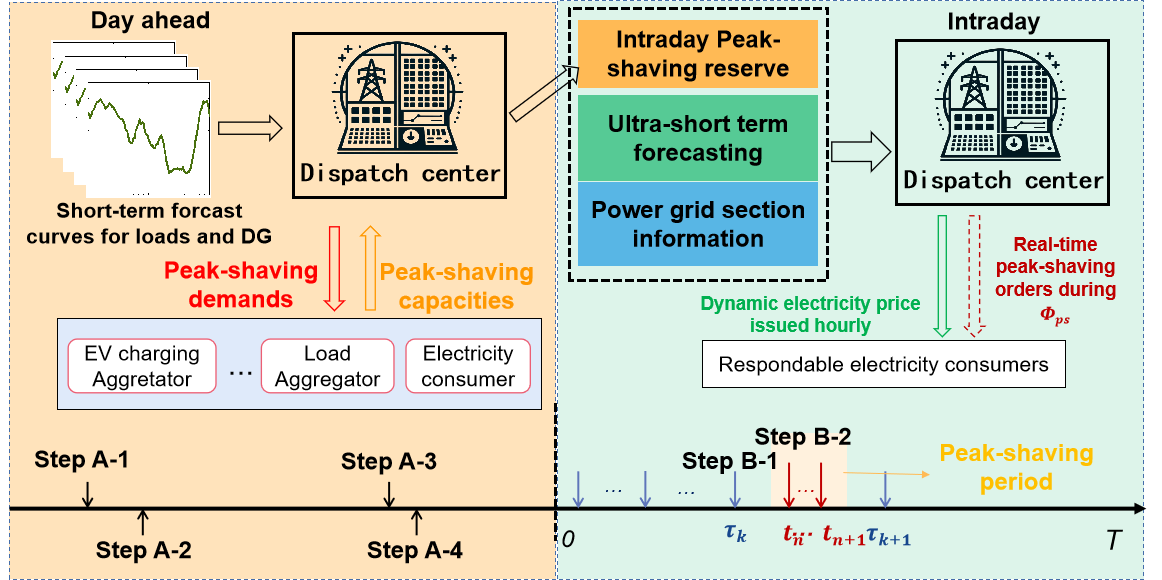
\includegraphics[width=1\linewidth]{figures/Demand respond.png}
    \caption{Demand response mechanism based on dynamic electricity price and real-time peak-shaving}
    \label{fig:Demand-response-mechanism}
\end{figure}
% \begin{figure}
%     \centering
%     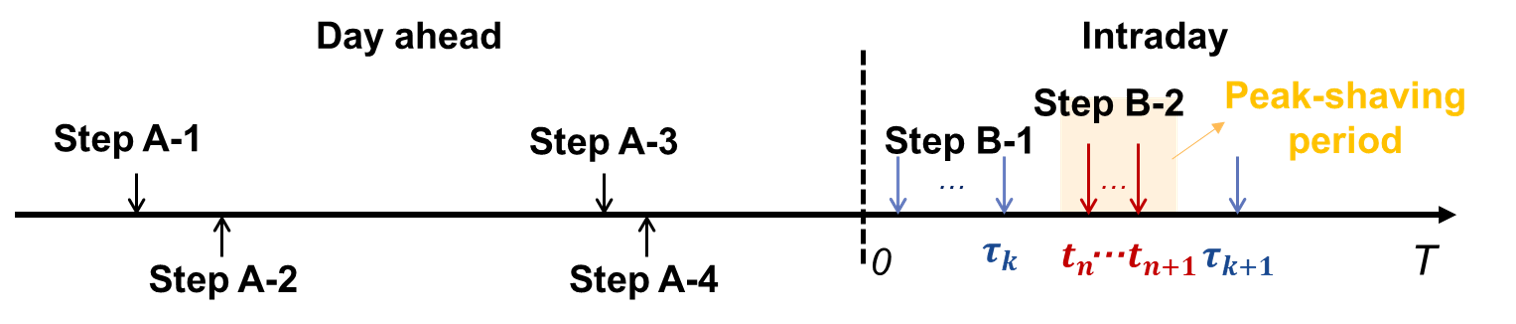
\includegraphics[width=1\linewidth]{figures/process of DR.png}
%     \caption{The dispatch and operation process of day-ahead and intra-day demand response}
%     \label{fig:The-processof DR}
% \end{figure}
\subsubsection{The dispatch process of demand response}
The dispatch and operation process of demand response is shown in  Fig. \ref{fig:Demand-response-mechanism}. Specifically, this process consists of six steps including:
\begin{itemize}
    \item Step A-1:Dispatch center of the power grid issues response offers to contracted power consumers or load aggregators based on the short-term forecast curves of load and new energy sources on the day before the operating day.
    \item Step A-2: Each customer feedback to the grid peak-shaving capacity in time slots according to its own forcasted power consumption or historical electricity consumption curves and grid's invitation information. 
    \item Step A-3: After the consumers responds to the invitations, the dispatch center preclears according to the principle of giving priority to the consumers with the highest response capacity, and the intraday peak-shaving reserve plan is available
    \item Step A-4: After the demand response market is pre-cleared, all responable consumers receive their own intraday peak-shaving reserve plan. And the peak-shaving reserve plan of the charging station at time t of the operating day is denoted as $b(t)$.
    \item Step B-1: During the operating day, the grid will dynamically issue electricity prices to guide customers' electricity consumption based on hourly ultra-short-term forecast curves of load and new energy sources. 
    \item Step B-2: In case of emergency regulation of the grid, such as local overloads or sudden spikes in demand, the dispatch center will issue real-time peak-shaving commands to responsive electricity consumers within the specified emergency regulation period, following the peak-shaving reserve plan.
\end{itemize}

\subsubsection{The dual-centralized control scheme under DR mechanisms}
We uses a dynamic real-time tariff mechanism, where electricity prices are set on an equal time cycle with parameter $\triangle_{\textrm{pr}}$. K is denoted as the total number of such price cycles during a day time T, for which the electricity prices are issued by the power grid dispatch center, and $\phi_{pr_{\textrm{ele}}}$ is the finite set for the electricity prices. Let $\tau_{k}$, with $k\in\phi_{K}=\{0,1,2,\ldots,K-1\}$, denote the starting point of the $k$th price cycle at $\tau_{0}=0$. For convenience, the electricity price during the $k$th price cycle is written as $pr_{\textrm{ele}}^{k}$, which remains the same until the end of the cycle, that is, $pr_{\textrm{ele}}(t)=pr_{\textrm{ele}}^{k}\in\phi_{pr_{\textrm{ele}}}$, $t\in[\tau_{k},\tau_{k+1})$. And, we set $\tau_{K}=T$. Therefore, the mechanism of dynamic electricity price is formualted as the sequence $\{(\tau_{k},pr_{\textrm{ele}}^{k})|k\in\phi_{K}\}$. 
Upon receiving dynamic electricity price information from the dispatch center, SPM sets the charging service price for the corresponding pricing period, denoted as $ pr_{\textrm{ser}}^{k}$ for the $k$th cycle. EV customer charging behaviors are known to be influenced by the station's service prices. Real-time service information, accessible through platforms like mobile apps, allows customers to promptly modify their charging plans, such as adjusting timing or opting for alternative stations. Consequently, we model the EV arrival rate as variable, dependent on the station's service price. This relationship is based on existing studies, specifically drawing from \citep{bao_approach_2022}, as follows:
\begin{equation}
\lambda(t)=\kappa(\lambda_{0}(t),pr_{\textrm{ser}}(t))(pr_{\textrm{ser}}(t)-pr_{0})+\lambda_{0}(t)
\label{eq:lambda_price}
\end{equation}
where $pr_{0}$ and $\lambda_{0}(t)$ represent the original fixed service price and the original arrival rate unaffected by service price; $pr_{ser}(t)$ is published service prices from SPM at time $t$; $\kappa(\lambda_{0}(t),pr_{\textrm{ser}}(t))$ is the coefficient of variation, whose value is less than $0$ and influenced by $\lambda_{0}(t)$ and $pr_{ser}(t)$.
Therefore, as the service price increases in a certain period, the number of charging customers will decrease in that period; conversely, the number of charging customers will increase.

Due to the existence of charging waiting, the arrival of the EV and the start of charging may not be in the same price cycle, so the actual charging price of the EV is is forced to be set to the minimum of the two service price:
\begin{equation}
pr_{j}(t)=\textrm{min}\left\{ pr_{\textrm{ser}}^{k_{a}},pr_{\textrm{ser}}^{k_{s}}\right\}
\end{equation}
where $pr_{j}(t)$ is the actual service price of the $j$th charging pile at time $t$; $k_{a}$ and $k_{s}$ are are the price periods
for the arrival and start of charging of EV at $cs_{j}$ at time $t$, respectively. And the service price for this EV is maintained until the EV ends its charging service.

When the grid is in emergency regulation periods, the dispatch center issues real-time peak-shaving commands to the load aggregators or electricity consumers. At time $t$, the peak-shaving commands received from the higher-level dispatch agency is recorded as $P_{\textrm{ps}}(t)$, and the amount of peak shaving will not exceed the intra-day peak-shaving reserve of the station, that is, $P_{\textrm{ps}}(t)\leq b(t)$. Considering the time requirement for real-time response, the charging station needs to complete load adjustment within 5 minutes after receiving the commands. Therefore, it is reasonable to assume that the minimum period for real-time peak-shaving commands is denoted as $\bigtriangleup_{\textrm{ps}}$ and $\bigtriangleup_{\textrm{ps}}\geq5$. To facilitate the operation, a operating day is divided into $N$ control cycles with $\bigtriangleup_{\textrm{ps}}$, and note that $t_{n}$, with $n\in\phi_{N}=\{0,1,2,\ldots,N-1\}$, denotes the starting point of the $n$th control cycle at $t_{0}=0$. Let $P_{ps}^{n}$ represents the peak-shaving command to be responded by the charging station during $n$th decision cycle. Obviously, in the $n$th cycle, if there exists a peak-shaving commands, such that $P_{\textrm{ps}}(t)\neq0$, then $P_{\textrm{ps}}^{n}=P_{\textrm{ps}}(t_{n})$; otherwise $P_{\textrm{ps}}^{n}=0$. Therefore, the peak-shaving mechanism for the charging station is formulated as the sequence $\{(t_{n},P_{\textrm{ps}}^{n})|n\in\phi_{N}\}$.

If the charging station receives a peak-shaving commands from the higher-level dispatch center, CPC will immediately adjust the charging powers of the charging piles according to the commands and current state of the station. Let the control variable of CPC during the $n$th control cycle be written as $P_{c}^{n}$, and the vector $P_{c}^{n}$ is the cut power of each charging pile, as shown in Eq. \ref{eq:CPC_action-1}.
% \begin{equation}
%     \begin{aligned}
%          P_{c}^{n}=\begin{cases}
%              \left\{ p_{1}^{c},p_{2}^{c},\cdots,p_{j}^{c},\cdots,p_{J}^{c}\right\}  & P_{\textrm{ps}}^{n}\neq 0\\
%              \left\{ 0,0,\cdots,0\right\}  & P_{\textrm{ps}}^{n}=0
%          \end{cases}\\
%         p_{j}^{c}\leq p_{j}(t_{n}),j\in\phi_{J}
%     \end{aligned}
%     \label{eq:CPC_action-1}
% \end{equation}
\begin{equation}
s.t.\begin{array}{c}
P_{c}^{n}=\begin{cases}
\left\{ p_{1}^{c},p_{2}^{c},\cdots,p_{j}^{c},\cdots,p_{J}^{c}\right\}  & P_{\textrm{ps}}^{n}\neq0\\
\left\{ 0,0,\cdots,0\right\}  & P_{\textrm{ps}}^{n}=0
\end{cases}\\
p_{j}^{c}\leq p_{j}(t_{n}),j\in\phi_{J}
\end{array}\label{eq:CPC_action-1}
\end{equation}

Then the charging powers of all charging piles change in line with the control variable $P_{c}^{n}$, as follows:
\begin{equation}
\begin{array}{c}
p_{j}(t_{n}^{+})=p_{j}(t_{n})-p_{j}^{c}\end{array}.\label{eq:CPC_action}
\end{equation}

\subsection{Performance criteria}

In this study, we adopt the viewpoint of a commercial charging facility, focusing on economic and peak regulation benefits as the primary performance indicators. This approach is twofold: firstly, it encompasses the daily operational profits derived from offering charging services to EV customers; secondly, it includes the benefits of peak shaving
achieved through compliance with directives from higher-level dispatching authorities.

Based on the cooperative bi-center control model, where SPM publishes service prices and CPC adjusts the charging powers of charging piles during peak-shaving periods, the operation benefit of the station in a finite horizon $T$ is  Eq. \ref{eq:operate_benefit}
\begin{equation}
R_{\textrm{ser}}=\sum_{k=0}^{K-1} \int_{\tau_{k}}^{\tau_{k+1}}\sum_{j=j}^{J}p_{j}(t)pr_{j}(t)dt.\label{eq:operate_benefit}
\end{equation}

And if the charging station responds to the peak-shaving commands from the the higher-level dispatch agency, it will be rewarded according to the actual response and baseline of the station. Let $P_{\textrm{bl}}(t)$ represents the baseline of the charging station, which is obtained
from the historical data of the typical operating days. The response power of the charging station is represented by $P_{\textrm{rsp}}\left(t\right)$, which is the value of the baseline power $P_{\textrm{bl}}(t)$ minus
the actual charging power of the station as following:
\begin{equation}
P_{\textrm{rsp}}(t)=P_{\textrm{bl}}(t)-\sum_{j=1}^{J}p_{j}(t).\label{eq:resp_power}
\end{equation}

In response to settlement, if the response power $P_{\textrm{rsp}}\left(t\right)$ exceeds $1.2P_{ps}(t)$, the excess will not be compensated. Therefore, the total response benefits $R_{\textrm{rsp}}$ of the charging station in a finite horizon $T$ is obtained from Eq. \ref{eq:response_benefits-1}.
\begin{equation}
R_{\textrm{rsp}}=\sum_{n=0}^{N-1}\textrm{sgn}\Bigl(P_{\textrm{ps}}^{n}\Bigr)\int_{t_{n}}^{t_{n+1}}\min\left\{ P_{\textrm{rsp}}(t),1.2P_{\textrm{ps}}(t)\right\} D_{\textrm{ps}}\varsigma_{\textrm{ps}}dt\label{eq:response_benefits-1}
\end{equation}

\begin{equation}
\varsigma_{\textrm{ps}}=\begin{cases}
1, & P_{\textrm{rsp}}(t)/P_{ps}(t)\geq0.8\\
0, & P_{\textrm{rsp}}(t)/P_{ps}(t)<0.8
\end{cases}\label{eq: coefficient of load response rate-1}
\end{equation}
Here, $\textrm{sgn}(\cdot)$ is an indicator function, that is, $\textrm{sgn}\Bigl(P_\textrm{ps}^{n}\Bigr)=0$ if $P_{ps}^{n}=0$; otherwise, $\textrm{sgn}\Bigl(P_\textrm{ps}^{n}\Bigr)=1$. $D_\textrm{ps}$ is the peak-shaving compensation price; $\varsigma_\textrm{ps}$ is the coefficient of load response rate, which has the value of $0$ when the load response rate is lower than 0.8 and the value of $1$ when it is not lower than $0.8$ as shown in Eq. \ref{eq: coefficient of load response rate-1}.

And considering the randomness of the EV flow and the intra-day peaking-shaving demands of the grid, the total expected economic return of the charging station is articulated as \ref{eq:spm_goal-1} . This is subsequently treated as the primary objective for the control unit SPM.
\begin{equation}
\mathit{Object_{\textrm{spm}}}=\mathbb{E}_{\lambda_{t},P_{\textrm{ps}}\left(t\right)}\Biggl[R_{\textrm{ser}}+R_{\textrm{rsp}}\Biggr]\label{eq:spm_goal-1}
\end{equation}

In addition, the response of CPC to real-time peak shaving commands from the higher-level dispatch agency may occasionally result in insufficient charging availability for some EV customers, potentially leading to a decline in customer satisfaction. We calculate the satisfaction cost for each user when an EV completes its charging and departs, basing this cost on the proportional increase in the vehicle's charging duration. We have established an exponential correlation between the satisfaction cost for EV users and the relative extension of their charging time. Consequently, during the $n$th decision-making cycle of the CPC, the cost associated with customer satisfaction is determined as follows:
\begin{equation}
\begin{array}{c}
c_{\textrm{sat}}(n)=\sum_{j=1}^{J}\sigma_{j}(\exp(\mu(t_{n}-I_{m_{j}}-T_{m_{j}}^{LB}))-1)\\
T_{m_{j}}^{LB}=\frac{(\bar{H}_{m_{j}}-H_{m_{j}}(I_{m_{j}}))E_{m_{j}}}{p_{m_{j}}^{max}}
\end{array}
\end{equation}
where if the EV on charging pile $cs_{j}$ leaves out during the $n$th decision cycle, then $\sigma_{j}=1$; if there is no EV on the charging pile or the EV is still charging without departure, then $\sigma_{j}=0$;
$\mu$ is a constant discount factor; $T_{m_{j}}^{LB}$ represents the time required for EV $m_{j}$ to charge at the rated power to meet the energy target.

Moreover, the cumulative satisfaction cost of customers over a finite horizon $T$ is represented as $C_\textrm{sat}$ and is derived from \ref{eq:cost_sat}.
\begin{equation}
C_{\textrm{sat}}=\sum_{n=0}^{N-1}c_{\textrm{sat}}(n).\label{eq:cost_sat}
\end{equation}

Concurrently, by considering the response gain $R_{rsp}$ of the charging station during grid peak periods, we can ascertain the expected objective for the control unit CPC in stochastic scenarios, as outlined in Eq.\ref{eq:spm_goal-1}.
\begin{equation}
Object_{\textrm{cpc}}=\mathbb{E}_{\lambda_{t},P_{\textrm{ps}}\left(t\right)}\Biggl[R_{\textrm{rsp}}-C_{\textrm{sat}}\Biggr].\label{eq:cpc_goal-1}
\end{equation}
\section{Solution via DHRL for EVCS}

In this section, we introduce a bi-layer collaborative optimization approach, leveraging DHRL, to tackle the challenges of dual-center control optimization. Acknowledging the uncertainty and non-linearity inherent in EV user behavior and intra-day real-time peak shaving demands, we have adopted a model-free optimization method using reinforcement learning. This bi-layer approach involves a sequential decision-making process, positioning the SPM and the CPC as the upper-layer and lower-layer agents, respectively. Within this hierarchical framework, the simulation model of the charging station is employed to generate operational samples by integration the actions of both agents. Furthermore, we introduce an enhanced optimization algorithm that incorporates an early feature fusion technique. This technique treats the amalgamated features as novel decision states
for the upper agent, thereby augmenting the efficiency of the learning
process.

\subsection{Bi-Layer Sequential Decision Process}

The cooperative dual-center control mode of the charging station includes
the service price formulation by the SPM and the real-time charging
power adjustment by the CPC. The SPM formulates the charging service
price for the next period based on the intra-day electricity price
information issued by the power grid, the states of the charging piles,
the waiting queue status, and\emph{ }peak-shaving reserve plan for
the station\emph{ }in the current price cycle. Meanwhile, the CPC
adjusts the charging powers based on the real-time peak-shaving commands
issued by the higher-level dispatch agency, the charging pile status
information, and the current charging service price. Therefore, considering
this logical relationship, we establish double agents based on the
hierarchical optimization method.

In order to synchronize with the decisions made at the upper level,
we construct a baseline sequence denoted as $\left\{ \left(\tau_{k},p_{\textrm{bl}}^{k}\right)|k\in\phi_{K}\right\} $,
where $p_{\textrm{bl}}^{k}=\int_{\tau_{k}}^{\tau_{k+1}}p_{\textrm{bl}}(t)dt$. To some extent, the baseline derived from the historical operation
data of the charging station can predict the load rate of the charging
piles for a future period of time. Similarly, the sequence of peak-shaving
reserve plan is compressed into $\left\{ \left(\tau_{k},B_{\textrm{ps}}^{k}\right)|k\in\phi_{K}\right\} $,
where $B_{\textrm{ps}}^{k}$ denotes the sum of peek- shaving reserve
during the time period $(\tau_{k},\tau_{k+1}]$, that is $B_{\textrm{ps}}^{k}=\int_{\tau_{k}}^{\tau_{k+1}}b(t)dt$.
Therefore, the state of the upper agent within the $k$th decision
period is defined as follows:

\begin{equation}
s_{\textrm{up}}^{k}=\left\{ k,p_{\textrm{bl}}^{k},pr_{\textrm{ele}}^{k},B_{\textrm{ps}}^{k},\bar{H}_{c}^{k},\bar{E}_{c}^{k},\bar{\mathbb{P}}_{c}^{k},\bar{p}_{c}^{k},\bar{H}_{w}^{k},\bar{E}_{w}^{k},\bar{\mathbb{P}}_{w}^{k}\right\} \label{eq:up_decision_state}
\end{equation}
where $\bar{H}_{\textrm{c}}^{k},\bar{E}_{\textrm{c}}^{k},\bar{\mathbb{P}}_{c}^{k}$ and $\bar{p}_{\textrm{c}}^{k}$ are the $J$-vectors representing the SoCs, battery capacities, rated charging powers and actual charging powers of the EVs served by the charging piles, respectively; $\bar{H}_{\textrm{w}}^{k},\bar{E}_{w}^{k},\bar{\mathbb{P}}_{w}^{k}$ are the $L$-vectors representing the SoCs, battery capacities and rated charging powers of the EV in the waiting spaces, respectively.

Now we assume that the upper agent takes actions according to the policy $\pi$, and the action determined by policy $\pi$ is denoted by $a_{\textrm{up}}^{k}=\pi(s_{\textrm{up}}^{k})$ at the $k$th upper-layer decision epoch $\tau_{k}$. Under action $a_{\textrm{up}}^{k}$, the
next event moves the system into a new state $s_{\textrm{up}}^{k+1}$ at decision epoch $\tau_{k+1}$. During this period, the reward of
upper agent is $r(s_{\textrm{up}}^{k},\pi(s_{\textrm{up}}^{k}),s_{\textrm{up}}^{k+1})$, which satisfies
\begin{equation}
r(s_{\textrm{up}}^{k},\pi(s_{\textrm{up}}^{k}),s_{\textrm{up}}^{k+1})=\underset{j\in\phi_{J}}{\sum}\int_{\tau_{k}}^{\tau_{k+1}}p_{j}\left(t\right)pr_{j}(t)+r_{\textrm{rsp}}(\tau_{k},\tau_{k+1})
% \begin{array}{r}
% r(s_{\textrm{up}}^{k},\pi(s_{\textrm{up}}^{k}),s_{\textrm{up}}^{k+1})=\underset{j\in\phi_{J}}{\sum}\int_{\tau_{k}}^{\tau_{k+1}}p_{j}\left(t\right)pr_{j}(t)\\
% +r_{\textrm{rsp}}(\tau_{k},\tau_{k+1})
% \end{array}
\label{eq:transit_reaward_upper}
\end{equation}
where $r_{\textrm{rsp}}(\tau_{k},\tau_{k+1})$ is the benefit obtained through participation in real-time peak shaving within the time period $(\tau_{k},\tau_{k+1}]$. We define the intersection of this time period with the peak-shaving period as $\phi_{\textrm{ps}}^{k}$ which
is the empty set if no commands is issued by the higher-level dispatch agency in that hour. Thus with reference to Eq. \ref{eq:response_benefits-1}, the response benefit during the $k$th price cycle can be obtained
as follows:

\begin{equation}
r_{\textrm{rsp}}(\tau_{k},\tau_{k+1})=\underset{t\in\phi_{\textrm{ps}}^{k}}{\int}\min\left\{ P_{\textrm{rsp}}(t),1.2P_{\textrm{ps}}(t)\right\} D_{\textrm{ps}}\varsigma_{\textrm{ps}}dt.
\end{equation}

Therefore, the tuple $<s_{\textrm{up}}^{k},a_{\textrm{up}}^{k},r(s_{\textrm{up}}^{k},a_{\textrm{up}}^{k},s_{\textrm{up}}^{k+1}),s_{\textrm{up}}^{k+1}>$ is recorded as a transition sample of upper agent.

As the CPC receives a real-time peak-shaving commands from the higher-level dispatch agency, it immediately adjust the operating powers of all the charging piles that are in use. Similar to the upper-layer decision-making process, we reconstruct the baseline sequence of the charging station according to the decision-making time of the lower agent, and denote it as $\left\{ \left(t_{n},p_{\textrm{bl}}^{n}\right)|n\in\phi_{N}\right\} $, where $p_{\textrm{bl}}^{n}=\int_{t_{n}}^{t_{n+1}}p_{\textrm{bl}}(t)dt$. And the sequence of service price is compressed into $\left\{ \left(t_{n},pr_{\textrm{ser}}^{n}\right)|n\in\phi_{N}\right\} $, where $pr_{\textrm{ser}}^{n}$ represents the service price during the time period $(t_{n},t_{n+1}]$. Therefore, the state of the lower agent within the $n$th decision period is defined as follows:
\begin{equation}
s_{\textrm{low}}^{n}=\{P_{\textrm{ps}}^{n},\bar{H}_{c}^{n},\bar{E}_{c}^{n},\bar{\mathbb{P}}_{c}^{n},\bar{p}_{c}^{n},\bar{H}_{w}^{n},\bar{E}_{w}^{n},\bar{\mathbb{P}}_{w}^{n},pr_{\textrm{ser}}^{n},p_{\textrm{bl}}^{n}\}.
\end{equation}

We define $\upsilon$ as the policy of the lower agent, with its determined action at the lower-layer decision epoch $t_{n}$ represented as $a_{\textrm{low}}^{n}=\upsilon(s_{\textrm{low}}^{n})$. The lower agent takes action $a_{\textrm{low}}^{n}$ under state $s_{\textrm{low}}^{n}$, resulting in the transition to a new state $s_{\textrm{low}}^{n+1}$ . During this period, the reward of lower agent is $r(s_{\textrm{low}}^{n},\upsilon(s_{\textrm{low}}^{n}),s_{\textrm{low}}^{n+1})$, $t_{n}<t\leq t_{n+1}$, which satisfies
\begin{equation}
r(s_{\textrm{low}}^{n},\upsilon(s_{\textrm{low}}^{n}),s_{\textrm{low}}^{n+1})=r_{\textrm{rsp}}(t_{n},t_{n+1})-c_{\textrm{sat}}\left(n\right).\label{eq:transit_reward_low}
\end{equation}

The tuple $<s_{\textrm{low}}^{n},a_{\textrm{low}}^{n},r(s_{\textrm{low}}^{n},a_{\textrm{low}}^{n+1},s_{\textrm{low}}^{n+1}),s_{\textrm{low}}^{n+1}>$ can describe the sequential decision-making process of the lower agent.


\subsection{Bi-Layer Collaborative Optimization Algorithm Based on TD3 and Dueling DQN}

The optimization variable of the upper-layer agent is the charging service price of EVs. The overall optimization objective of the upper-layer agent, as shown in Eq. \ref{eq:spm_goal-1}, can be transformed into
the accumulated transition reward within a finite horizon $T$. The total finite-horizon reward of upper agent when starting from $s_{up}^{0}$ and taking action following the policy $\pi$, is composed of the accumulated rewards of $K$ transitions:
\begin{equation}
V^{\pi}(s_{\textrm{up}})=E_{\pi,\lambda_{k}}\Biggl[\sum_{k=0}^{K-1}r(s_{\textrm{up}}^{k},\pi(s_{\textrm{up}}^{k}),s_{\textrm{up}}^{k+1})\Biggl|s_{\textrm{up}}=s_{\textrm{up}}^{0}\Biggr]\label{eq:up_v(s)}
\end{equation}

The optimization variable of the lower-layer agent is the charging powers of the charging piles, and its goal is to maximize the sum of peak-shaving benefits during peak hours and user satisfaction weighted together. Like the upper-layer agent, the overall objective of the lower-layer agent is converted into the cumulative transfer reward within peak-shaving period $\phi_{ps}$. The total finite-horizon reward of lower agent when starting from $s_{low}^{0}$ and taking action following the policy $\upsilon$, is composed of the accumulated rewards of $N$ transitions:
\begin{equation}
V^{\upsilon}(s_{\textrm{low}})=E_{\upsilon,\lambda_{n},P_{\textrm{ps}}^{n}}\Biggl[\sum_{n=0}^{N-1}r(s_{\textrm{low}}^{n},\upsilon(s_{\textrm{low}}^{n}),s_{\textrm{low}}^{n+1})
\Biggl|s_{\textrm{low}}=s_{\textrm{low}}^{0}\Biggr]
% \begin{array}{r}
% V^{\upsilon}(s_{\textrm{low}})=E_{\upsilon,\lambda_{n},P_{\textrm{ps}}^{n}}\Biggl[\sum_{n=0}^{N-1}r(s_{\textrm{low}}^{n},\upsilon(s_{\textrm{low}}^{n}),s_{\textrm{low}}^{n+1})\\
% \Biggl|s_{\textrm{low}}=s_{\textrm{low}}^{0}\Biggr]
% \end{array}
\label{eq:low_V(s)}
\end{equation}


Furthermore, with the initial state of charging station stochastic, the following finite-horizon expected returns are considered as the optimization objective function of the upper-layer agent and lower-layer
agent, respectively:
\begin{equation}
V^{\pi}=E_{\pi,\lambda_{k},s_{\textrm{up}}^{0}}\Biggl[\sum_{k=0}^{K-1}r(s_{\textrm{up}}^{k},a_{\textrm{up}}^{k},s_{\textrm{up}}^{k+1})\Biggr]\label{eq:up_agrnt_goal}
\end{equation}

\begin{equation}
V^{\upsilon}=E_{\upsilon,\lambda_{n},P_{ps}^{n},s_{\textrm{low}}^{0}}\Biggl[\sum_{n=0}^{N-1}r(s_{\textrm{low}}^{n},\upsilon(s_{\textrm{low}}^{n}),s_{\textrm{low}}^{n+1})\Biggr]\label{eq:low_agrnt_goal}
\end{equation}

According to formula \ref{eq:up_v(s)} and \ref{eq:low_V(s)}, we define the Q functions for the upper and lower-layer agents, respectively. Q function, denoted as $Q^{*}(s,a)$, is the expected accumulated
return of taking action $a$, thereafter, following the policy $*$. Thus, $Q^{\pi}(s_{up}^{k},a_{up}^{k})$ is Q function for the state
action pair $\left\langle s_{up}^{k},a_{up}^{k}\right\rangle $ of upper-layer agent under policy $\pi$ as shown in formula \ref{eq:up_Q}.
\begin{equation}
Q^{\pi}(s_{\textrm{up}}^{k},a_{\textrm{up}}^{k})=E_{\pi,\lambda_{k}}\Biggl[r(s_{\textrm{up}}^{k},a_{\textrm{up}}^{k},s_{\textrm{up}}^{k+1})+V^{\pi}(s_{\textrm{up}}^{k+1})\Biggr]\label{eq:up_Q}
\end{equation}

And $Q^{\upsilon}(s_{\textrm{low}}^{n},a_{\textrm{low}}^{n})$ is Q function for the state action pair $\left\langle s_{\textrm{low}}^{n},a_{\textrm{low}}^{n}\right\rangle $ of lower-layer agent under policy $\upsilon$, as shown in \ref{eq:low_Q}.

\begin{equation}
Q^{\upsilon}(s_{\textrm{low}}^{n},a_{\textrm{low}}^{n})=E_{\upsilon,\lambda_{n},P_{\textrm{ps}}^{n}}\Biggl[r(s_{\textrm{low}}^{n},a_{\textrm{low}}^{n},s_{\textrm{low}}^{n+1})
+V^{\upsilon}(s_{\textrm{low}}^{n+1})\Biggr]
% \begin{array}{r}
% Q^{\upsilon}(s_{\textrm{low}}^{n},a_{\textrm{low}}^{n})=E_{\upsilon,\lambda_{n},P_{\textrm{ps}}^{n}}\Biggl[r(s_{\textrm{low}}^{n},a_{\textrm{low}}^{n},s_{\textrm{low}}^{n+1})\\
% +V^{\upsilon}(s_{\textrm{low}}^{n+1})\Biggr]
% \end{array}
\label{eq:low_Q}
\end{equation}


In our study, we focus on optimizing charging station strategies, considering the stochastic behavior of EV flow and the requirements for intra-day peak-shaving, with the goal of maximizing overall returns.
The unpredictability of EV arrivals and the need for real-time optimization pose significant challenges to traditional, model-based sequential decision-making methods. To address these challenges, our approach
incorporates a dual-centralized control scheme within the charging station framework, employing DHRL. This method includes the application of the Dueling Deep Q-Network (Dueling DQN) algorithm for the upper-layer agent and the Twin Delayed Deep Deterministic policy gradient (TD3) algorithm for the lower-layer agent.
\begin{figure*}[h]
    \centering
    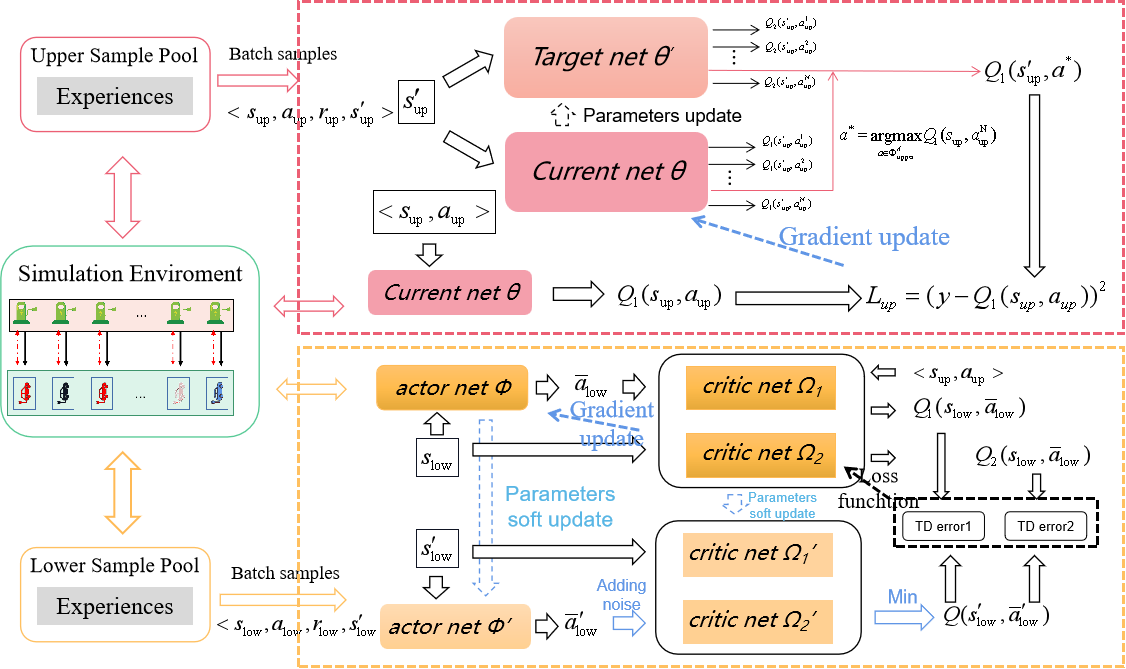
\includegraphics[width=0.95\linewidth]{figures/Learning framwork.png}
    \caption{Learning framework with bi-layer architecture based on Dueling DQN and TD3}
    \label{fig:DRL-based-learning-framwwork}
\end{figure*}

Reinforcement Learning (RL), as an interactive learning paradigm with the environment, has been widely used for optimizing action policy. The ultimate goal of RL is to achieve maximum cumulative rewards, as represented by Eq. \ref{eq:up_agrnt_goal} and \ref{eq:low_agrnt_goal}. To obtain the requisite learning samples, we have designed a comprehensive simulation environment that simulates the operation of fast charging stations, EV arrival events, and grid peak-shaving demand. At each decision epoch, the agent observes the current state of the environment and selects the action based on the current policy. The agent then transitions to the next state and receives the corresponding rewards. In this study, we define the state transfer that occurs when two agents interact with the environment as the learning samples of the agents,
which are represented by $<s_{\textrm{up}}^{k},a_{\textrm{up}}^{k},r_{\textrm{up}}^{k},s_{\textrm{up}}^{k+1}>$ and $<s_{\textrm{low}}^{n},a_{\textrm{low}}^{n},r_{\textrm{low}}^{n},s_{\textrm{low}}^{n+1}>$,
respectively. We establish $B_{\textrm{up}}$ and $B_{\textrm{low}}$ as the sample experience pools of the two agents with respective capacities of $N_{\textrm{pool}}^{\textrm{up}}$ and $N_{\textrm{pool}}^{\textrm{low}}$. When these pools are full, a random batch of samples is drawn for training and updating agent parameters, with $b_{\text{up}}$ and $b_{\text{low}}$ indicating the mini-batch sizes for upper and lower agents. The RL architecture, based on a bi-layer learning structure, is presented in Fig. \ref{fig:DRL-based-learning-framwwork}.

Dueling DQN is a deep reinforcement learning algorithm that is effective in solving problems with discrete action spaces \cite{pmlr-v48-wangf16}. Building upon Q-learning, Dueling DQN splits the Q-value function
into two parts: a value function $V(s)$ for the state $s$ and an advantage function $A(s,a)$ that represents the relative advantage of each action with respect to the state as shown in Eq. \ref{eq:dueling_dqn_qvalue}.
Through a specific Dueling network architecture, these two functions are recombined,\emph{ }when the relative advantage functions for each action are similar, the state value function can better support decision-making.
And in this study, to prevent the overestimation of Q values, we adopt a double Q-net structure, consisting of a target net and a current net, denoted as $Q_{tar}(s_{\textrm{up}}^{k},a_{\textrm{up}}^{k},\theta^{'})$ and $Q_{cur}(s_{\textrm{up}}^{k},a_{\textrm{up}}^{k},\theta)$ respectively, where $\theta$ and $\theta^{'}$ represent the parameters of the target and current nets. The two Q-nets are mutually independent, with the current network responsible for interacting with the simulation environment to generate samples $<s_{\textrm{low}}^{n},a_{\textrm{low}}^{n},r_{\textrm{low}}^{n},s_{\textrm{low}}^{n+1}>$. The target network evaluates the Q value of the next state based on the data in the sample pool, and then obtains the loss function to update the current network parameters as shown in formula \ref{eq:duelingDQN_loss}. After every $L_{DQN}$ learning steps, the parameters of the target network will be updated according to formula \ref{eq:dqn_para_update} with $\vartheta_{DQN}$ as the update ratio coefficient.
\begin{equation}
Q^{\pi}(s_{\textrm{up}}^{k},a_{\textrm{up}}^{k})=V^{\pi}(s_{\textrm{up}}^{k})+A^{\pi}(s_{\textrm{up}}^{k},a_{\textrm{up}}^{k})\label{eq:dueling_dqn_qvalue}
\end{equation}

with
\[
E_{a_{up}^{k}\sim\pi(s_{up}^{k})}\Biggl[A^{\pi}(s_{up}^{k},a_{up}^{k})\Biggr]=0
\]

\begin{equation}
Loss(\theta)=\Biggl(Q_{cur}(s_{up}^{k},a_{up}^{k},\theta)-(r_{low}^{k}+
\gamma Q_{tar}(s_{up}^{k+1},\underset{a_{up}}{\textrm{argmax}}Q_{cur}(s_{up}^{k+1},a_{up},\theta),\theta^{'}))\Biggr)^{2}b_{\textrm{up}}^{\textrm{-1}}
% \begin{array}{c}
% Loss(\theta)=\Biggl(Q_{cur}(s_{up}^{k},a_{up}^{k},\theta)-(r_{low}^{k}+\\
% \gamma Q_{tar}(s_{up}^{k+1},\underset{a_{up}}{\textrm{argmax}}Q_{cur}(s_{up}^{k+1},a_{up},\theta),\theta^{'}))\Biggr)^{2}b_{\textrm{up}}^{\textrm{-1}}
% \end{array}
\label{eq:duelingDQN_loss}
\end{equation}

\begin{equation}
\theta^{'}=\vartheta_{DQN}\theta^{'}+(1-\vartheta_{DQN})\theta\label{eq:dqn_para_update}
\end{equation}


The TD3 (Twin Delayed Deep Deterministic Policy Gradient) algorithm, an actor-critic based RL algorithm, excels in optimizing continuous action spaces with its rapid training capabilities. The actor network,
represented as $\upsilon(s_{\textrm{low}}^{n},\varphi)$, parameterizes the policy $\upsilon$, which determines actions corresponding to
the current state $s_{low}^{n}$, where $\varphi$ denotes its network parameters. The critic net is used to evaluate the Q value of the state-action pair $<s_{\textrm{low}}^{n},a_{\textrm{low}}^{n}>$ with $a_{\textrm{low}}^{n}=\upsilon(s_{\textrm{low}}^{n},\varphi)$ here. In order to reduce the bias of the evaluation, TD3 adopts a double critic structure with two critic nets denoted as $Q^{\upsilon}(s_{\textrm{low}}^{n},a_{\textrm{low}}^{n},\Omega_{1})$
and $Q^{\upsilon}(s_{\textrm{low}}^{n},a_{\textrm{low}}^{n},\Omega_{2})$, where $\varOmega_{1}$ and $\varOmega_{2}$ are two network parameters. To ensure the stability of the training, a total of 6 independent neural networks need to be created: actor net $\upsilon(s_{\textrm{low}}^{n},\varphi)$ and two critic nets $Q^{\upsilon}(s_{\textrm{low}}^{n},a_{\textrm{low}}^{n},\Omega_{1})$, $Q^{\upsilon}(s_{\textrm{low}}^{n},a_{\textrm{low}}^{n},\Omega_{2})$, target actor net $\upsilon(s_{\textrm{low}}^{n},\varphi^{'})$ and two target critic nets $Q^{\upsilon}(s_{\textrm{low}}^{n},a_{\textrm{low}}^{n},\Omega_{1}^{'})$, $Q^{\upsilon}(s_{\textrm{low}}^{n},a_{\textrm{low}}^{n},\Omega_{2}^{'})$.

The two critic nets are trained simultaneously and the loss functions are as following:
\begin{equation}
\begin{array}{c}
Loss(\Omega_{i})=E\Biggl[\Biggl(Q^{\upsilon}(s_{\textrm{low}}^{n},a_{\textrm{low}}^{n},\Omega_{i})-y_{td3}\Biggr)^{2}\Biggr]\\
y_{td3}=r_{\textrm{low}}^{n}+\underset{i=1,2}{\textrm{min}}(Q^{\upsilon}(s_{\textrm{low}}^{n+1},\upsilon(s_{\textrm{low}}^{n+1},\varphi)+\epsilon,\Omega_{i}))\\
\epsilon\sim clip(N(0,\sigma),-c,c).
\end{array}
\end{equation}


And the actor net update its parameters using the deterministic policy gradient \cite{pmlr-v80-fujimoto18a}:
\begin{equation}
\nabla_{\varphi}J(\varphi)=b_{\textrm{low}}^{\textrm{-1}}\sum\nabla_{a_{\textrm{low}}^{n}}Q^{\upsilon}(s_{\textrm{low}}^{n},a_{\textrm{low}}^{n},\Omega_{1})\Biggl|_{a_{\textrm{low}}^{n}}
\nabla_{\varphi}\upsilon(s_{\textrm{low}}^{n},\varphi)
% \begin{array}{r}
% \nabla_{\varphi}J(\varphi)=b_{\textrm{low}}^{\textrm{-1}}\sum\nabla_{a_{\textrm{low}}^{n}}Q^{\upsilon}(s_{\textrm{low}}^{n},a_{\textrm{low}}^{n},\Omega_{1})\Biggl|_{a_{\textrm{low}}^{n}}\\
% \nabla_{\varphi}\upsilon(s_{\textrm{low}}^{n},\varphi)
% \end{array}
\label{eq:policy_gra}
\end{equation}


After every $L_{TD3}$ learning steps, the parameters of the three target nets will be updated according to formula \ref{eq:dqn_para_update} with $\vartheta_{TD3}$ as the update ratio coefficient.

\begin{equation}
\begin{array}{c}
\varphi^{'}=\vartheta_{TD3}\varphi^{'}+(1-\vartheta_{TD3})\varphi\\
\Omega_{i}^{'}=\vartheta_{TD3}\Omega_{i}^{'}+(1-\vartheta_{TD3})\Omega_{i},i=1,2
\end{array}
\end{equation}


\subsection{Improved Optimization Algorithm based on FF-DHRL}

Optimal decision-making in agents requires precise and efficient environmental perception. However, practical scenarios often present the agent's decision state with missing or redundant information, impeding action strategy optimization. According to Eq. \ref{eq:up_decision_state}, the upper-layer agent's decision state includes the charging station state and external grid data, where states like rated power, battery
capacity, and SoC display weak correlation and high dimensionality, minimally impacting decision-making. To address this, we employ feature fusion technology in the Dueling DQN network's input layer, as illustrated
in Fig\ref{fig:Network-FF-DDQN}. This approach consolidates relevant state features, enabling the agent to learn and make decisions from a fused and streamlined state representation.

\begin{figure}[tb]
    \centering
    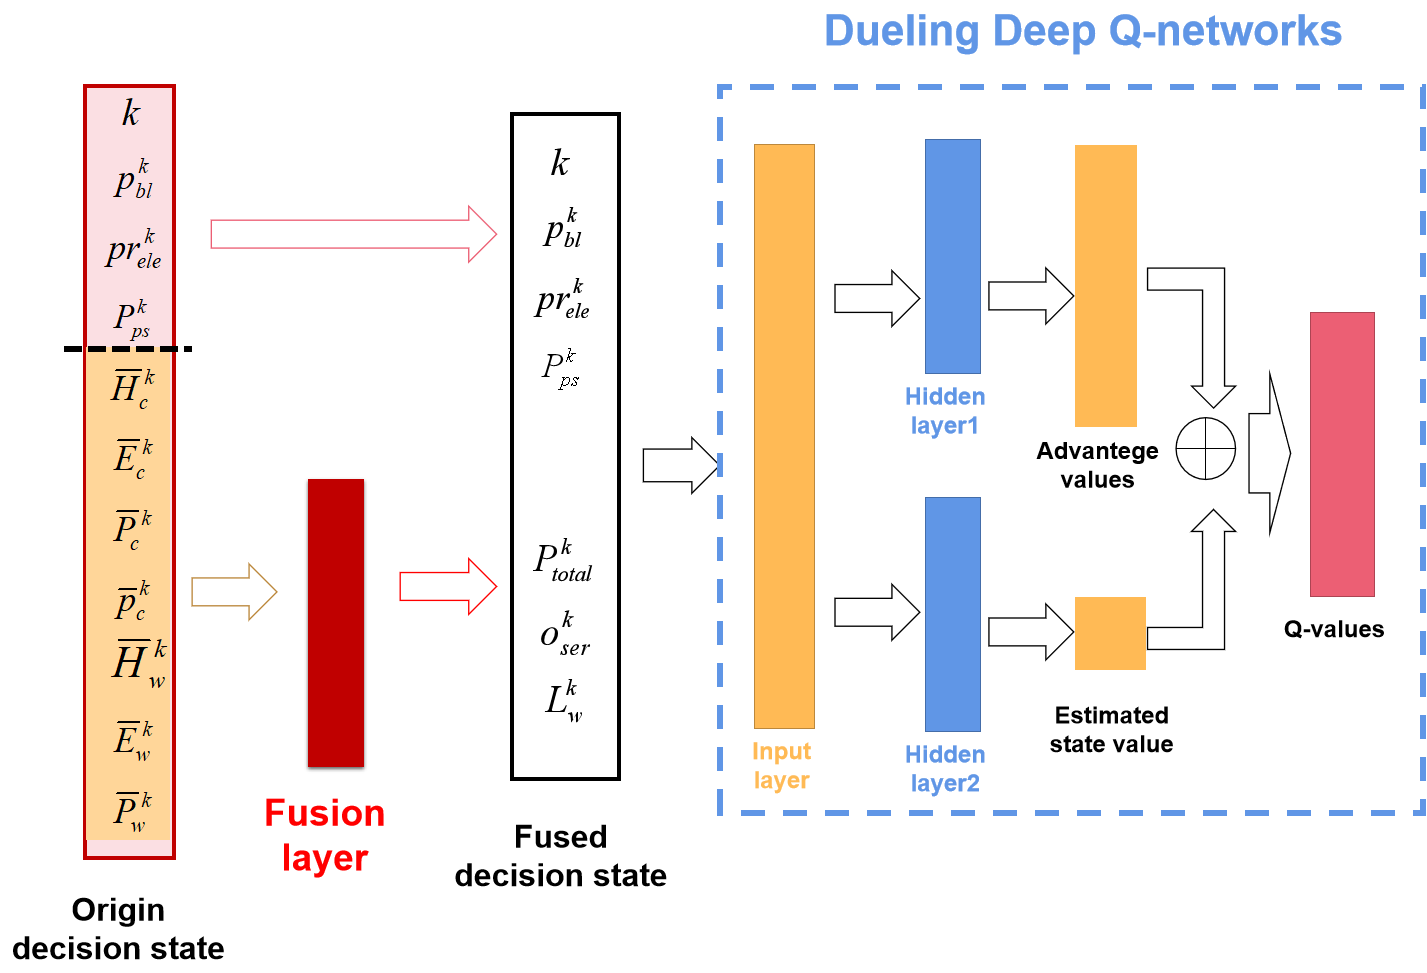
\includegraphics[width=1\linewidth]{figures/Feature Fusion.png}
    \caption{Network structure of Dueling DQN using feature fusion}
    \label{fig:Network-FF-DDQN}
\end{figure}

The features of the EVs served by charging piles are analyzed. The actual charging power $\bar{p}_{c}^{k}$ of the $J$ charging piles is superimposed and fused to the total load value $P_{\textrm{total}}^{k}$ of the station at the $k$th decision epoch:

\begin{equation}
P_{\textrm{total}}^{k}=\biggl\Vert\bar{p}_{c}^{k}\biggr\Vert_{1}
\end{equation}

To optimize economic benefits at the upper layer, the agent needs to effectively respond to two scenarios. In times of low electricity prices, if there is idle capacity in the charging piles, lowering service prices can encourage more usage, thus enhancing pile utilization and service revenue. Conversely, during high electricity price periods with significant remaining working time, the station can strategically
increase service prices to moderate the load, selectively reducing user charging and boosting response revenue. Consequently, the charging time of each pile is more critical than the State of Charge (SoC),
battery capacity, or rated power of EVs. To compute the remaining charging time $\Gamma_{c}^{k}$ for EVs at each pile, we use the state information $H_{c}^{k}$, $E_{c}^{k}$, and $p_{c}^{k}$ at the $k$th decision epoch, applying the following formula:

\begin{equation}
\Gamma_{c}^{k}=(\tilde{H}-H_{c}^{k})\odot E_{c}^{k}\odot\Upsilon_{c}\cdot\eta^{-1}\label{eq:cp_remain_charging_time}
\end{equation}

\begin{equation}
\varUpsilon_{c}(j)=\begin{cases}
1/p_{j}(t_{k})\text{,} & p_{j}(t_{k})\neq0\\
0, & p_{j}(t_{k})=0
\end{cases},1\leq j\leq J\label{eq:r_c_j}
\end{equation}
where the symbol $\odot$ is Hadamard product representing multiplication of the elements of the vectors at each corresponding position; the vector $\varUpsilon_{c}$ consists of the elements $\varUpsilon_{c}(j)$ and is a $J$-dimensional vector. Each element $\varUpsilon_{c}(j)$ can be calculated by Eq. \ref{eq:r_c_j}.

In a similar vein, we can acquire the anticipated required charging time of EVs in the waiting queue by leveraging the state features $H_{w}^{k}$, $E_{w}^{k}$ and $P_{w}^{k}$ at the $k$th decision instance, denoted as $\Gamma_{w}^{k}$.

\begin{equation}
\Gamma_{w}^{k}=(\tilde{H}-H_{w}^{k})\odot E_{w}^{k}\odot\Upsilon_{w}\cdot\eta^{-1}
\end{equation}
\begin{equation}
\varUpsilon_{w}(l)=\begin{cases}
1/P_{l}(t_{k}) & P_{l}(t_{k})\neq0\\
0 & P_{l}(t_{k})=0
\end{cases},1\leq l\leq L.\label{eq:r_w_l}
\end{equation}
where the $L$-dimensional vector $\varUpsilon_{w}$ consists of the elements $\varUpsilon_{w}(l)$. Each element $\varUpsilon_{w}(l)$ can be calculated by Eq. \ref{eq:r_w_l}.



To further express the utilization of charging piles within the decision cycle, we define the proportion of the current total remaining charging time of the station relative to the maximum service capacity available within the decision cycle as the charging time utilization rate of the station in the current decision cycle. We then use it as a new fused feature, denoted as $o_{\textrm{ser}}^{k}$, which is defined by the following equation:

\begin{equation}
o_{\textrm{ser}}^{k}=\frac{\biggl(\biggl\Vert\Gamma_{c}^{k}\biggr\Vert_{1}+\biggl\Vert\Gamma_{w}^{k}\biggr\Vert_{1}\biggr)}{J\times\triangle_{\textrm{pr}}}
\end{equation}
where the denominator represents the maximum service time of $J$ charging piles during the decision cycle $\triangle_{\textrm{pr}}$, and the numerator represents the sum of the expected remaining charging time for charging piles and EVs in the queue under the current state.

During the process, the information about the number of EVs waiting in the queue was blurred out. Therefore, we added the number of EVs waiting in the queue, denoted as $L_{w}^{k}$, as a new feature
to the fused state. The value of $L_{w}^{k}$ can be obtained from the queue state vector $H_{w}^{k}$:
\begin{equation}
L_{w}^{k}=\sum_{l=1}^{L}\mathbb{I}(H_{w}^{k}(l)\neq0)
\end{equation}
where$\mathbb{I}$ is an indicator function which takes the value 1 when $H_{w}^{k}(l)$ is not equal to 0, and 0 otherwise.

Now the fused decision stated of the upper agent is
\begin{equation}
\bar{s}_{\textrm{up}}^{k}=\biggl\{ k,p_{\textrm{bl}}^{k},pr_{\textrm{ele}}^{k},B_{\textrm{ps}}^{k},P_{\textrm{total}}^{k},o_{\textrm{ser}}^{k},L_{w}^{k}\biggr\}
\end{equation}
where scalar $P_{\textrm{total}}^{k}$, $o_{\textrm{ser}}^{k}$ and $L_{w}^{k}$ are the actual load, charging time utilization rate and queue length of the station at $k$th epoch, respectively. It is obvious that the space of the upper decision state after fusing the features is smaller than the space of the origin, i.e., $\biggl|\bar{s}_{up}^{k}\biggr|<\biggl|s_{up}^{k}\biggr|$.
The agent learns and trains based on the fused features state, which can improve the exploration efficiency of the policy space. The subsequent case studies have verified that compared to the original decision state, using the fused decision state can significantly improve the learning speed of the agent.

\section{Case Study}
%%\label{}
\subsection{Settings of Simulations}

In this system, we consider the charging piles can serve three types
of EVs, and the parameters of such EVs are listed in Tab. \ref{tab:THE-PARAMETERS-EV}  and the charging efficiency of the charging pile is $\eta=0.9$. It is assumed that when EV arrives, three types of EVs  have the same probability. All EVs' initial SoCs satisfy a uniform distribution on the interval $[0.1,0.4]$ and their target SoC is $\tilde{H}=0.9$. In consideration of the mobility characteristics of EVs users during weekdays, we divide the
arrival rate of EV flow into four stages and the time periods corresponding to the four arrival rates are listed in Table\ref{tab:THE-ARRIVAL-RATE}. Based on this, the initial state of the charging station is randomly set to the case of a few charging piles working at the initial moment of the day, and the average value of the simulated load curve for 1000 days is used as the baseline of the charging station, as shown
in Fig.\ref{fig:The-baseline}.
% It is assumed that when an EV arrives, three types of EVs have the same
% probability, that is $\lambda_{1}(t)=\lambda_{2}(t)=\lambda_{3}(t)$.

\begin{table}[h]
    \centering
\caption{The parameters of EVs}
\label{tab:THE-PARAMETERS-EV}
    \begin{tabular}{c r r} \hline  
         EV type&  $E_{m}^{max}$(\kwh)& $P_{m}^{max}$(\kwh)\\ \hline  
         $m=1$& 110 & 350\\  
         $m=2$& 80   &160 \\   
         $m=3$&  140& 280\\ \hline 
    \end{tabular}
\end{table}

\begin{table}[hp]
\caption{The arrival rate of EV flow}
\label{tab:THE-ARRIVAL-RATE}
\noindent \centering{}%
\begin{tabular}{>{\centering}p{0.18\columnwidth}>{\raggedleft}p{0.14\columnwidth}>{\raggedleft}p{0.14\columnwidth}>{\raggedleft}p{0.2\columnwidth}>{\raggedleft}p{0.1\columnwidth}}
\hline
Time periods & 8:00\textendash 9:00 & 15:00\textendash 19:00 & 1:00\textendash 7:00 and 20:00\textendash 24:00 & Else time\tabularnewline
\hline
Arrival rate & 0.8 & 1.0 & 0.3 & 0.5\tabularnewline
\hline
\end{tabular}
\end{table}



The parameters of intra-day grid tariff and real-time peaking used
in the experiments are referenced from the 2022 commercial and industrial
tariff and demand response implementation plan for Anhui Province,
China. The electricity tariffs are shown in Tables\ref{tab:TOU-TARIFF}.
Furthermore, we set the decision cycles of the upper and lower agents
to $\Delta_\textrm{pr}=60\textrm{min}$and $\Delta_\textrm{ps}=5\textrm{min}$,
respectively. In this experiment, two real-time peak-shaving periods
are set, denoted as $\phi_{ps}^{1}$ and $\phi_{ps}^{2}$. The first
peak-shaving period $\phi_{ps}^{1}$ has a duration of 1 hour, while
the second peak-shaving period $\phi_{ps}^{2}$ has a duration of
2.5 hours. The peak-shaving compensation price is set to $D_\textrm{ps}=\textrm{12\kwh}$.
The start times and real-time peak-shaving demands for each peak-shaving
period are random variables. We assume that the start times for the
two peak-shaving periods, denoted as$T_\textrm{ps}^{1}$ and $T_\textrm{ps}^{2}$,
follow a normal distribution, each limited to the time periods $[120,132]$and
$[186,198]$ respectively, as shown in Eq. \ref{eq:start_time_ps}
. The real-time peak-shaving quantity follows a uniform distribution,
and its mean and range of variation are shown in Fig. \ref{fig:Real-time-peak-shaving}.

\begin{equation}
\begin{array}{c}
T_{ps}^{1}\sim clip(N(\mu=126,\sigma^{2}=0.8),120,132)\\
T_{ps}^{2}\sim clip(N(\mu=192,\sigma^{2}=0.8)186,198)
\end{array}\label{eq:start_time_ps}
\end{equation}

\begin{figure}[hp]
    \centering
    \subfloat[\label{fig:The-baseline}The baseline of charging station]{
    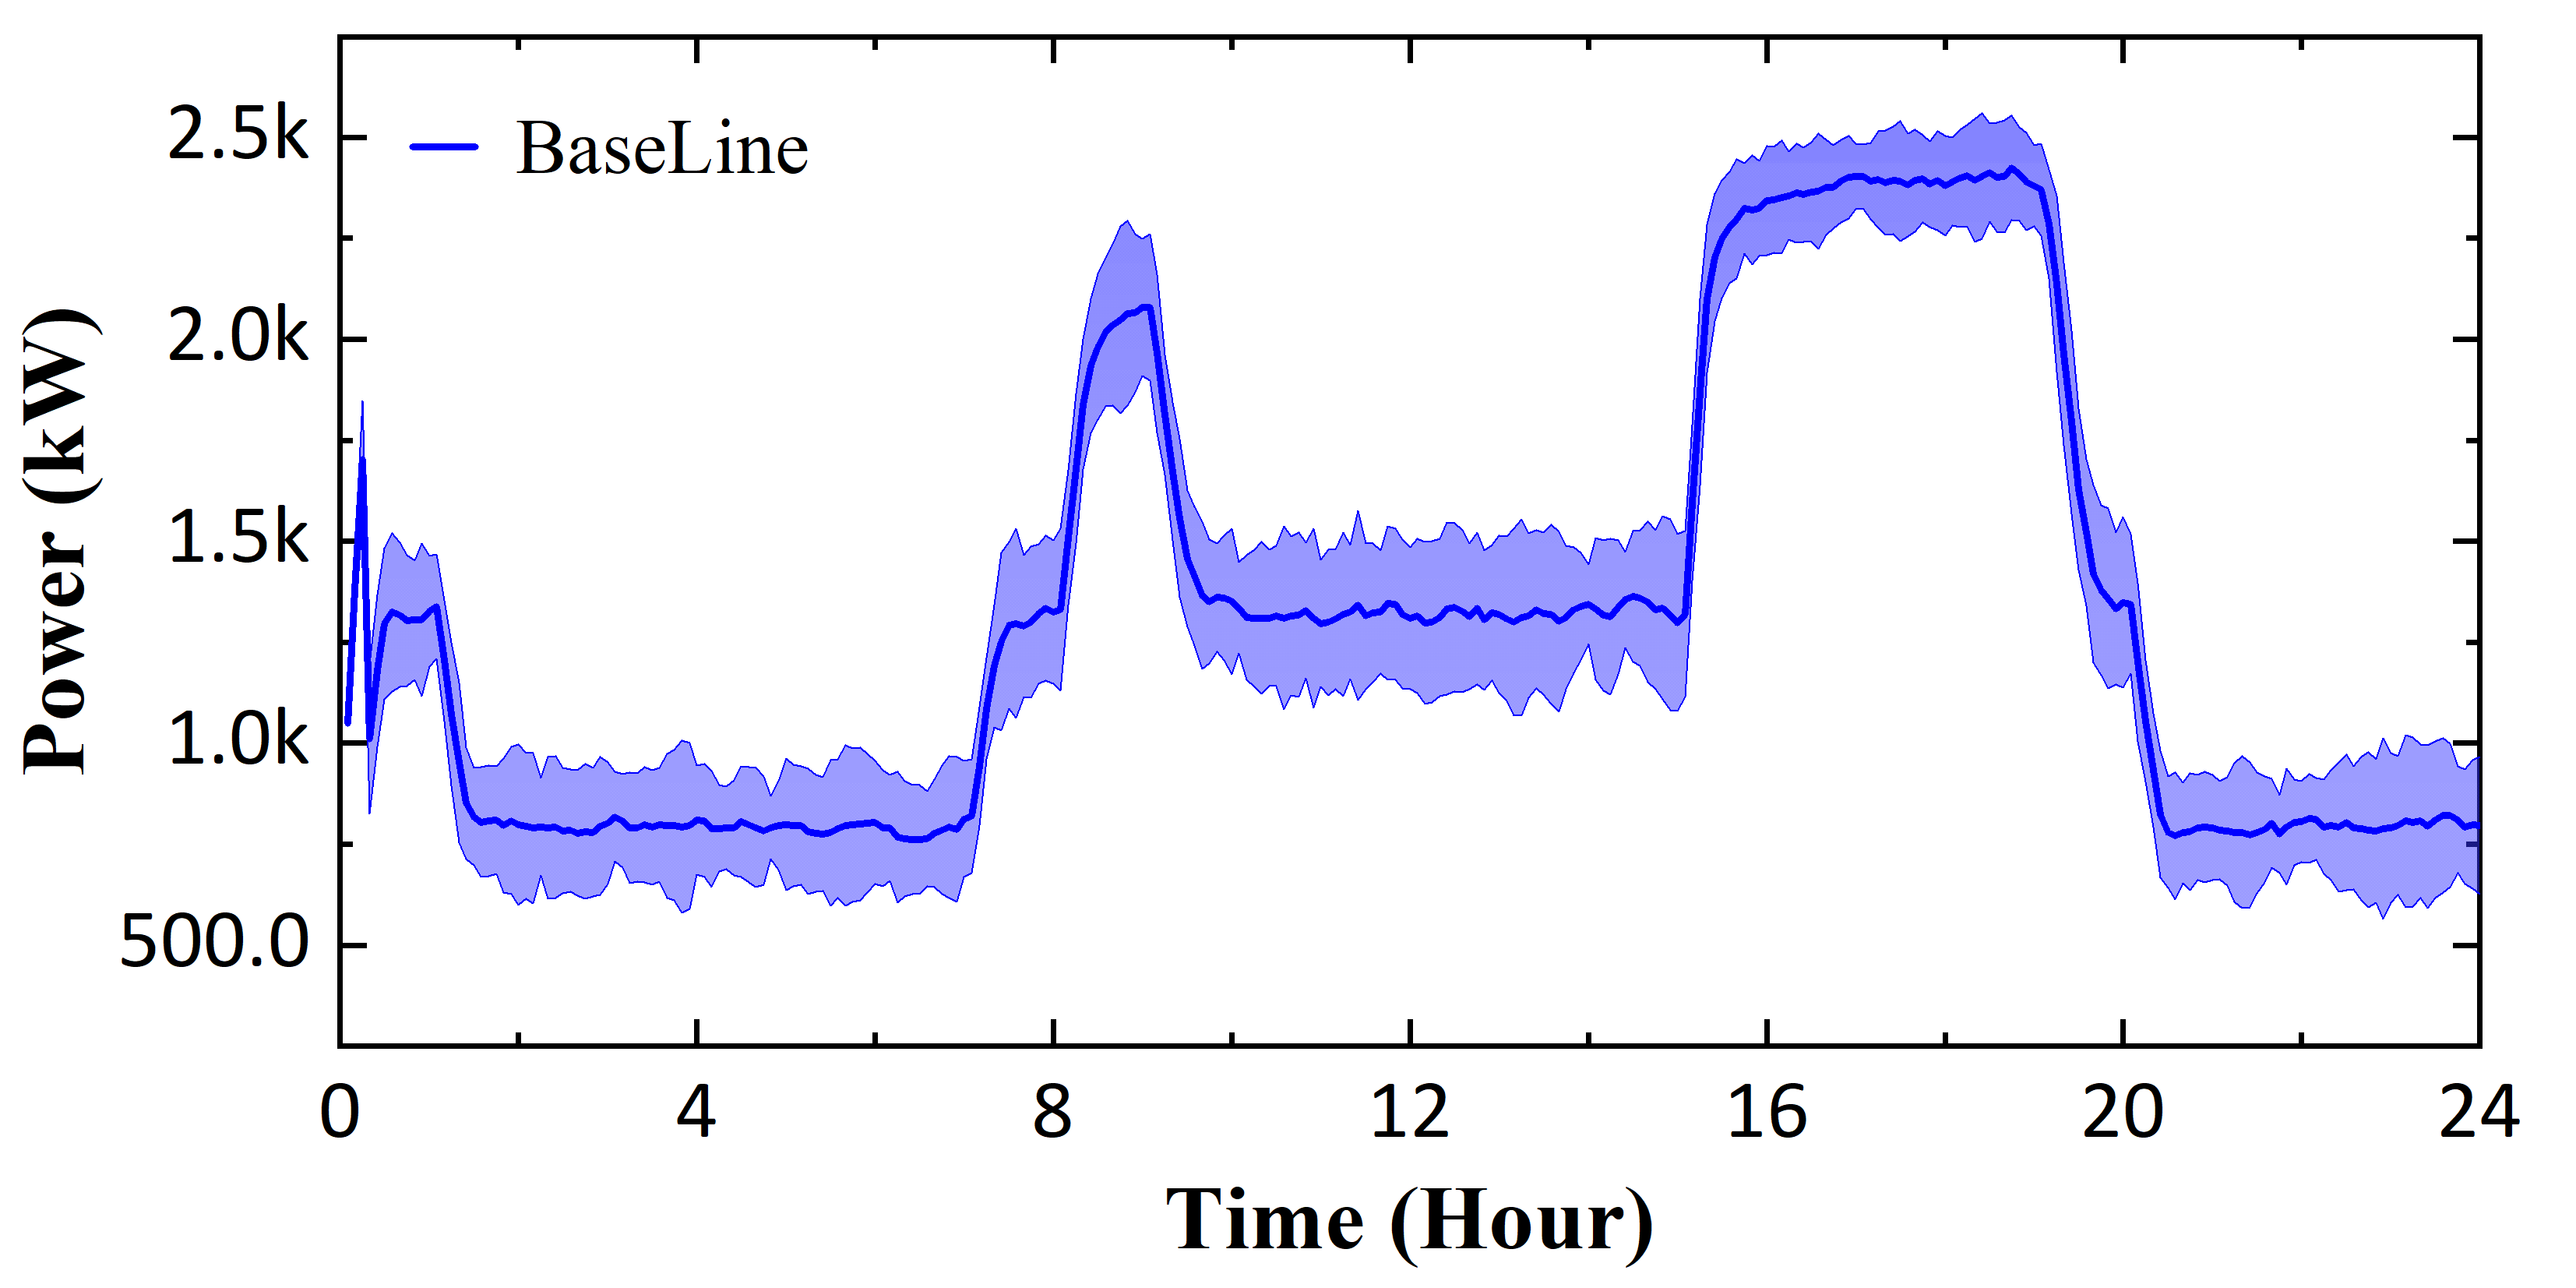
\includegraphics[width=0.48\linewidth]{figures/baseline}}
    \hfill % 可选的,用于在子图之间添加空格
    \subfloat[\label{fig:Real-time-peak-shaving}Real-time peak shaving commands]{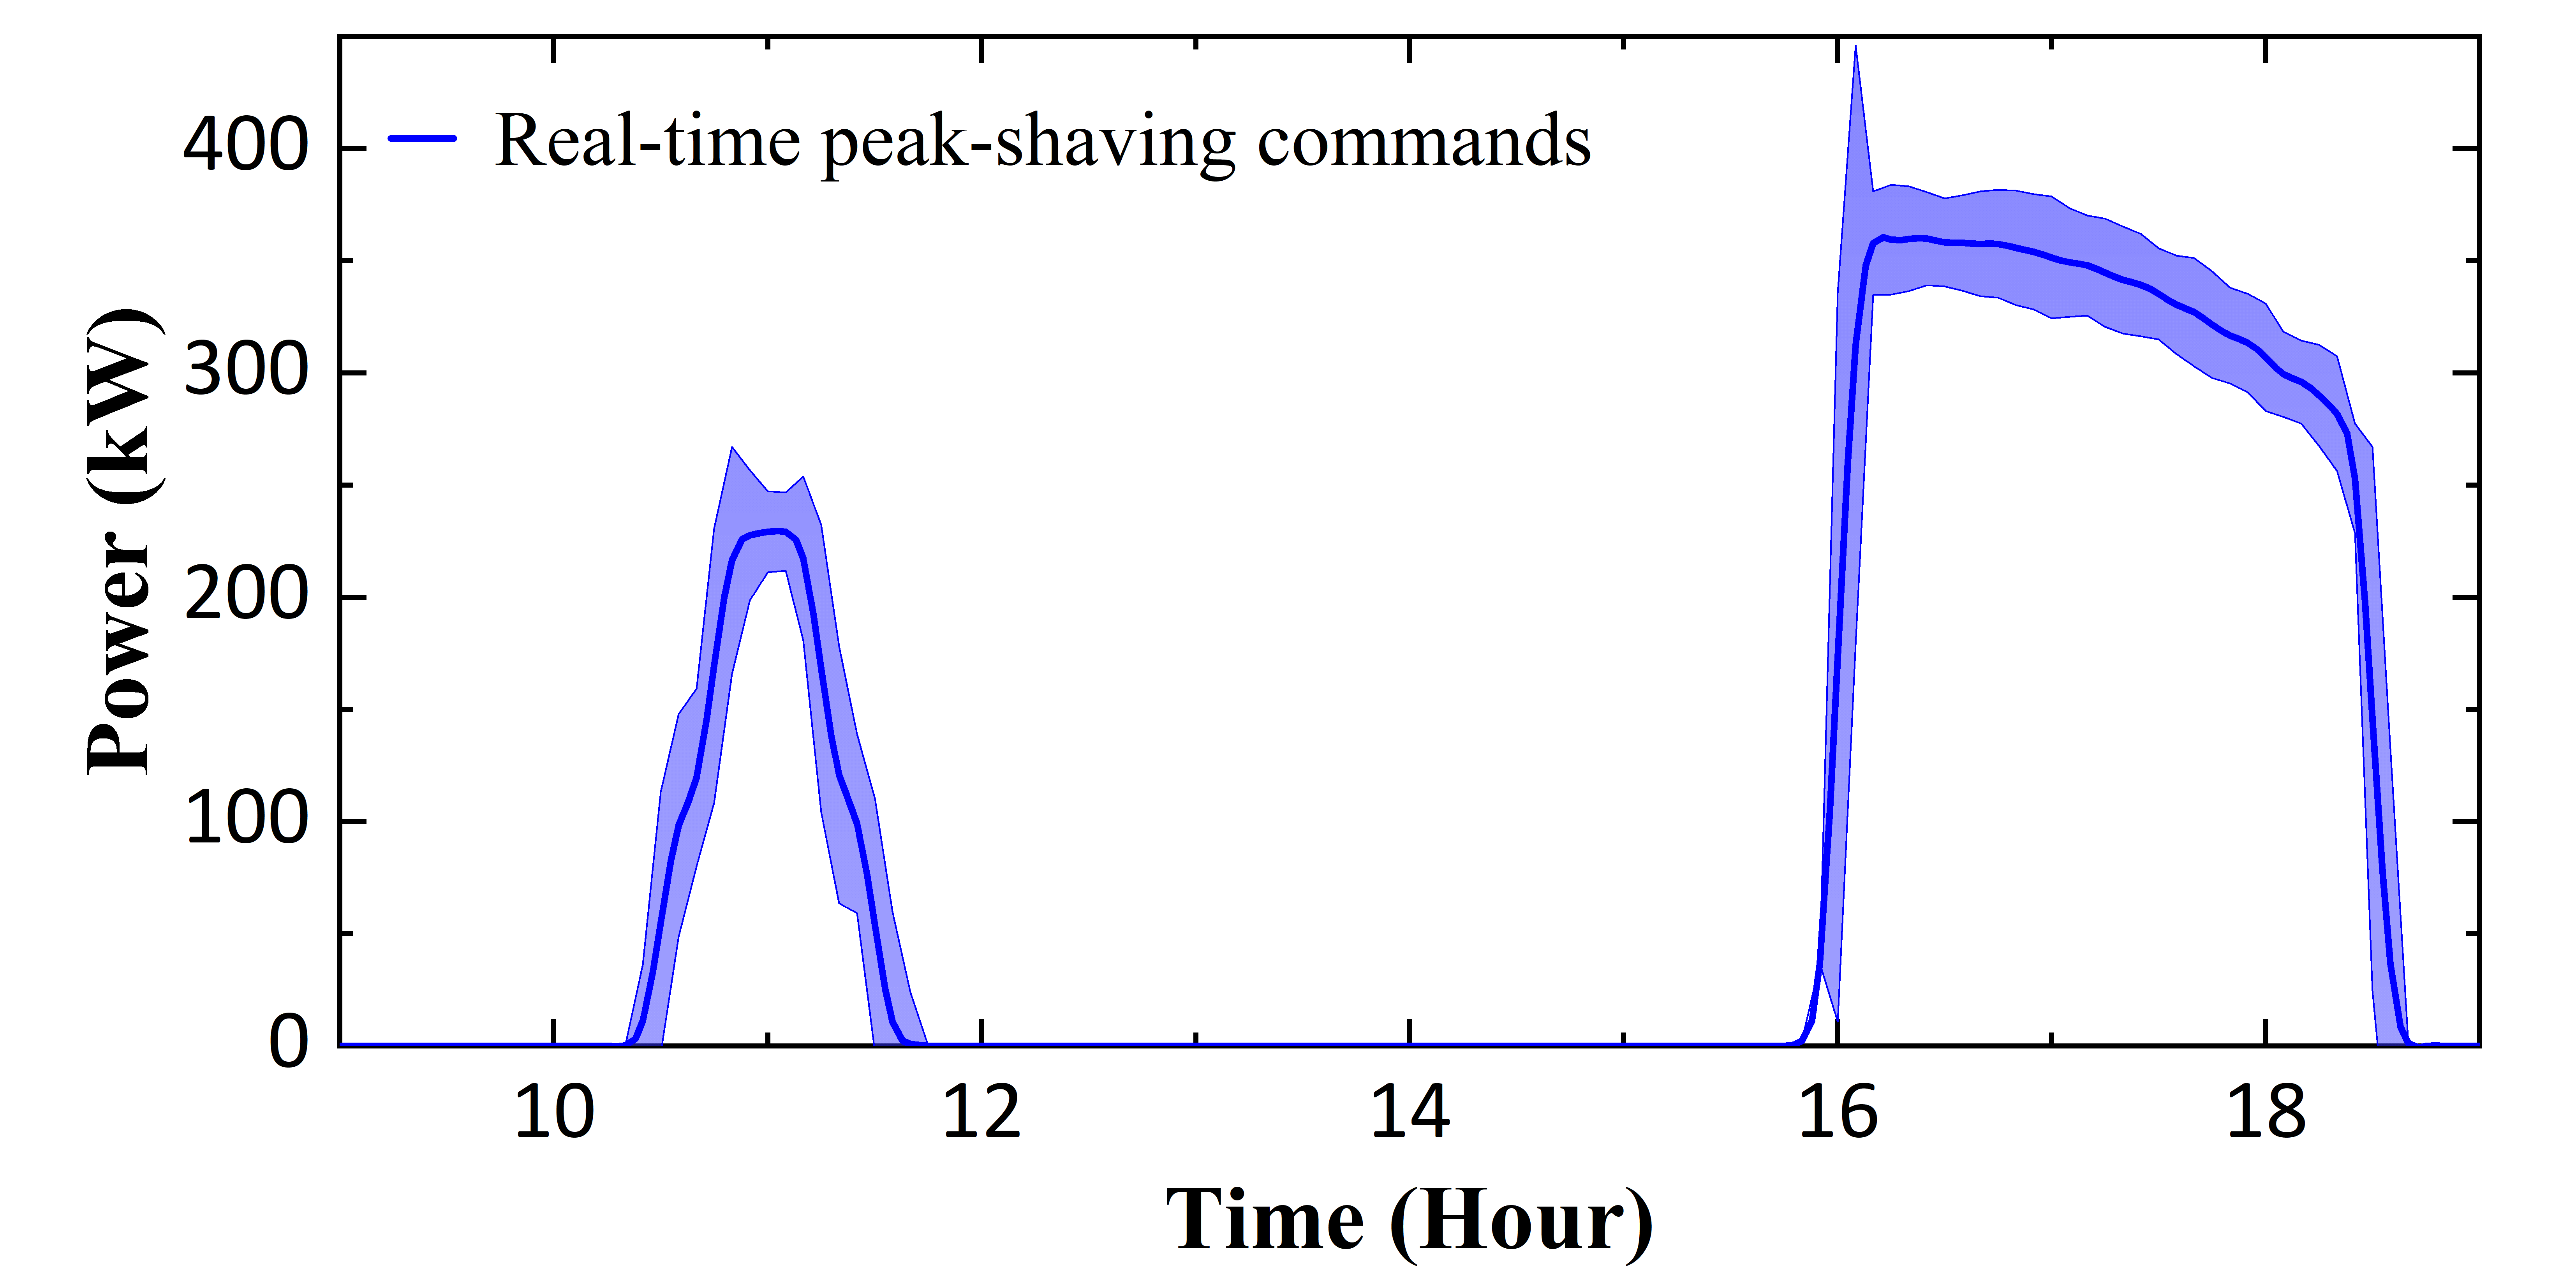
\includegraphics[width=0.48\linewidth]{figures/ps_orders}}
    \caption{The baseline of charging station and real-time peak-shaving commands. }
    \label{fig:Baseline_and_Orders}
\end{figure}
% This curve is derived from taking
% the average of 1000 days of simulated operation based on the set arrival
% rate and initial state. The blue curve represents the mean of 1000
% samples, while the blue shaded area indicates the 95\% confidence
% interval.
\begin{table}[thp]
\caption{Electricity price of power grid}
\label{tab:TOU-TARIFF}
\noindent \centering{}%
\begin{tabular}{>{\centering}m{0.15\columnwidth}>{\raggedleft}m{0.2\columnwidth}>{\raggedleft}m{0.23\columnwidth}>{\raggedleft}m{0.2\columnwidth}}
\hline
Execution period  & \raggedleft{}10:00-12:00 and 14:00-19:00 & \raggedleft{}8:00-10:00, 12:00-14:00 and 19:00-21:00 & \raggedleft{}0:00-8:00 and 21:00-24:00\tabularnewline
\hline
Electricity Price
& \raggedleft{}1.4 (\$/kW.h)  & \raggedleft{}1 (\$/kW.h)  & \raggedleft{}0.8 (\$/kW.h) \tabularnewline
\hline
\end{tabular}
\end{table}

The hyperparameter of algorithms must be artificially set before training
begins. The hyperparameters were determined after several experiments,
as shown in Table\ref{tab:Parameters-learning}. 
% and the network structures of the agent were shown in Table xx

\begin{table}[h]
\caption{Parameters-setting for the learning}
\label{tab:Parameters-learning}
\begin{centering}
\begin{tabular}{lclc}
\hline
Parameter & Value & Parameter & Value\tabularnewline
\hline
Learning rate & 0.0001 & Upper buffer size & 100000\tabularnewline
Soft update rate & 0.001 & Upper batch size & 526\tabularnewline
Episode length & 32 & Lower buffer size & 100000\tabularnewline
Step size & 100 & Lower batch size & 128\tabularnewline
% Upper buffer size & 100000\tabularnewline
% Upper batch size & 526\tabularnewline
% Lower buffer size & 100000\tabularnewline
% Lower batch size & 128\tabularnewline
\hline
\end{tabular}
\par\end{centering}
\end{table}



\subsection{Effectiveness of Feature Fusion}

To verify the effectiveness of feature fusion in enhancing the algorithm,
we have established three sets of comparative optimization methods.
The first group consists of DHRL without utilizing fused feature.
For the second group, we introduce a commonly used state processing
technology in queuing systems to modify the input features of the
upper-level agent. This method is named FF1-DHRL. The specific state
processing procedure is presented in Appendix A. The third group consists
of the improved method proposed in this paper, named FF2-DHRL. These
three methods will be trained and evaluated under the same parameter
settings and random seeds.

\begin{figure}[hp]
\begin{centering}
\subfloat[Upper-layer objection]{\begin{centering}
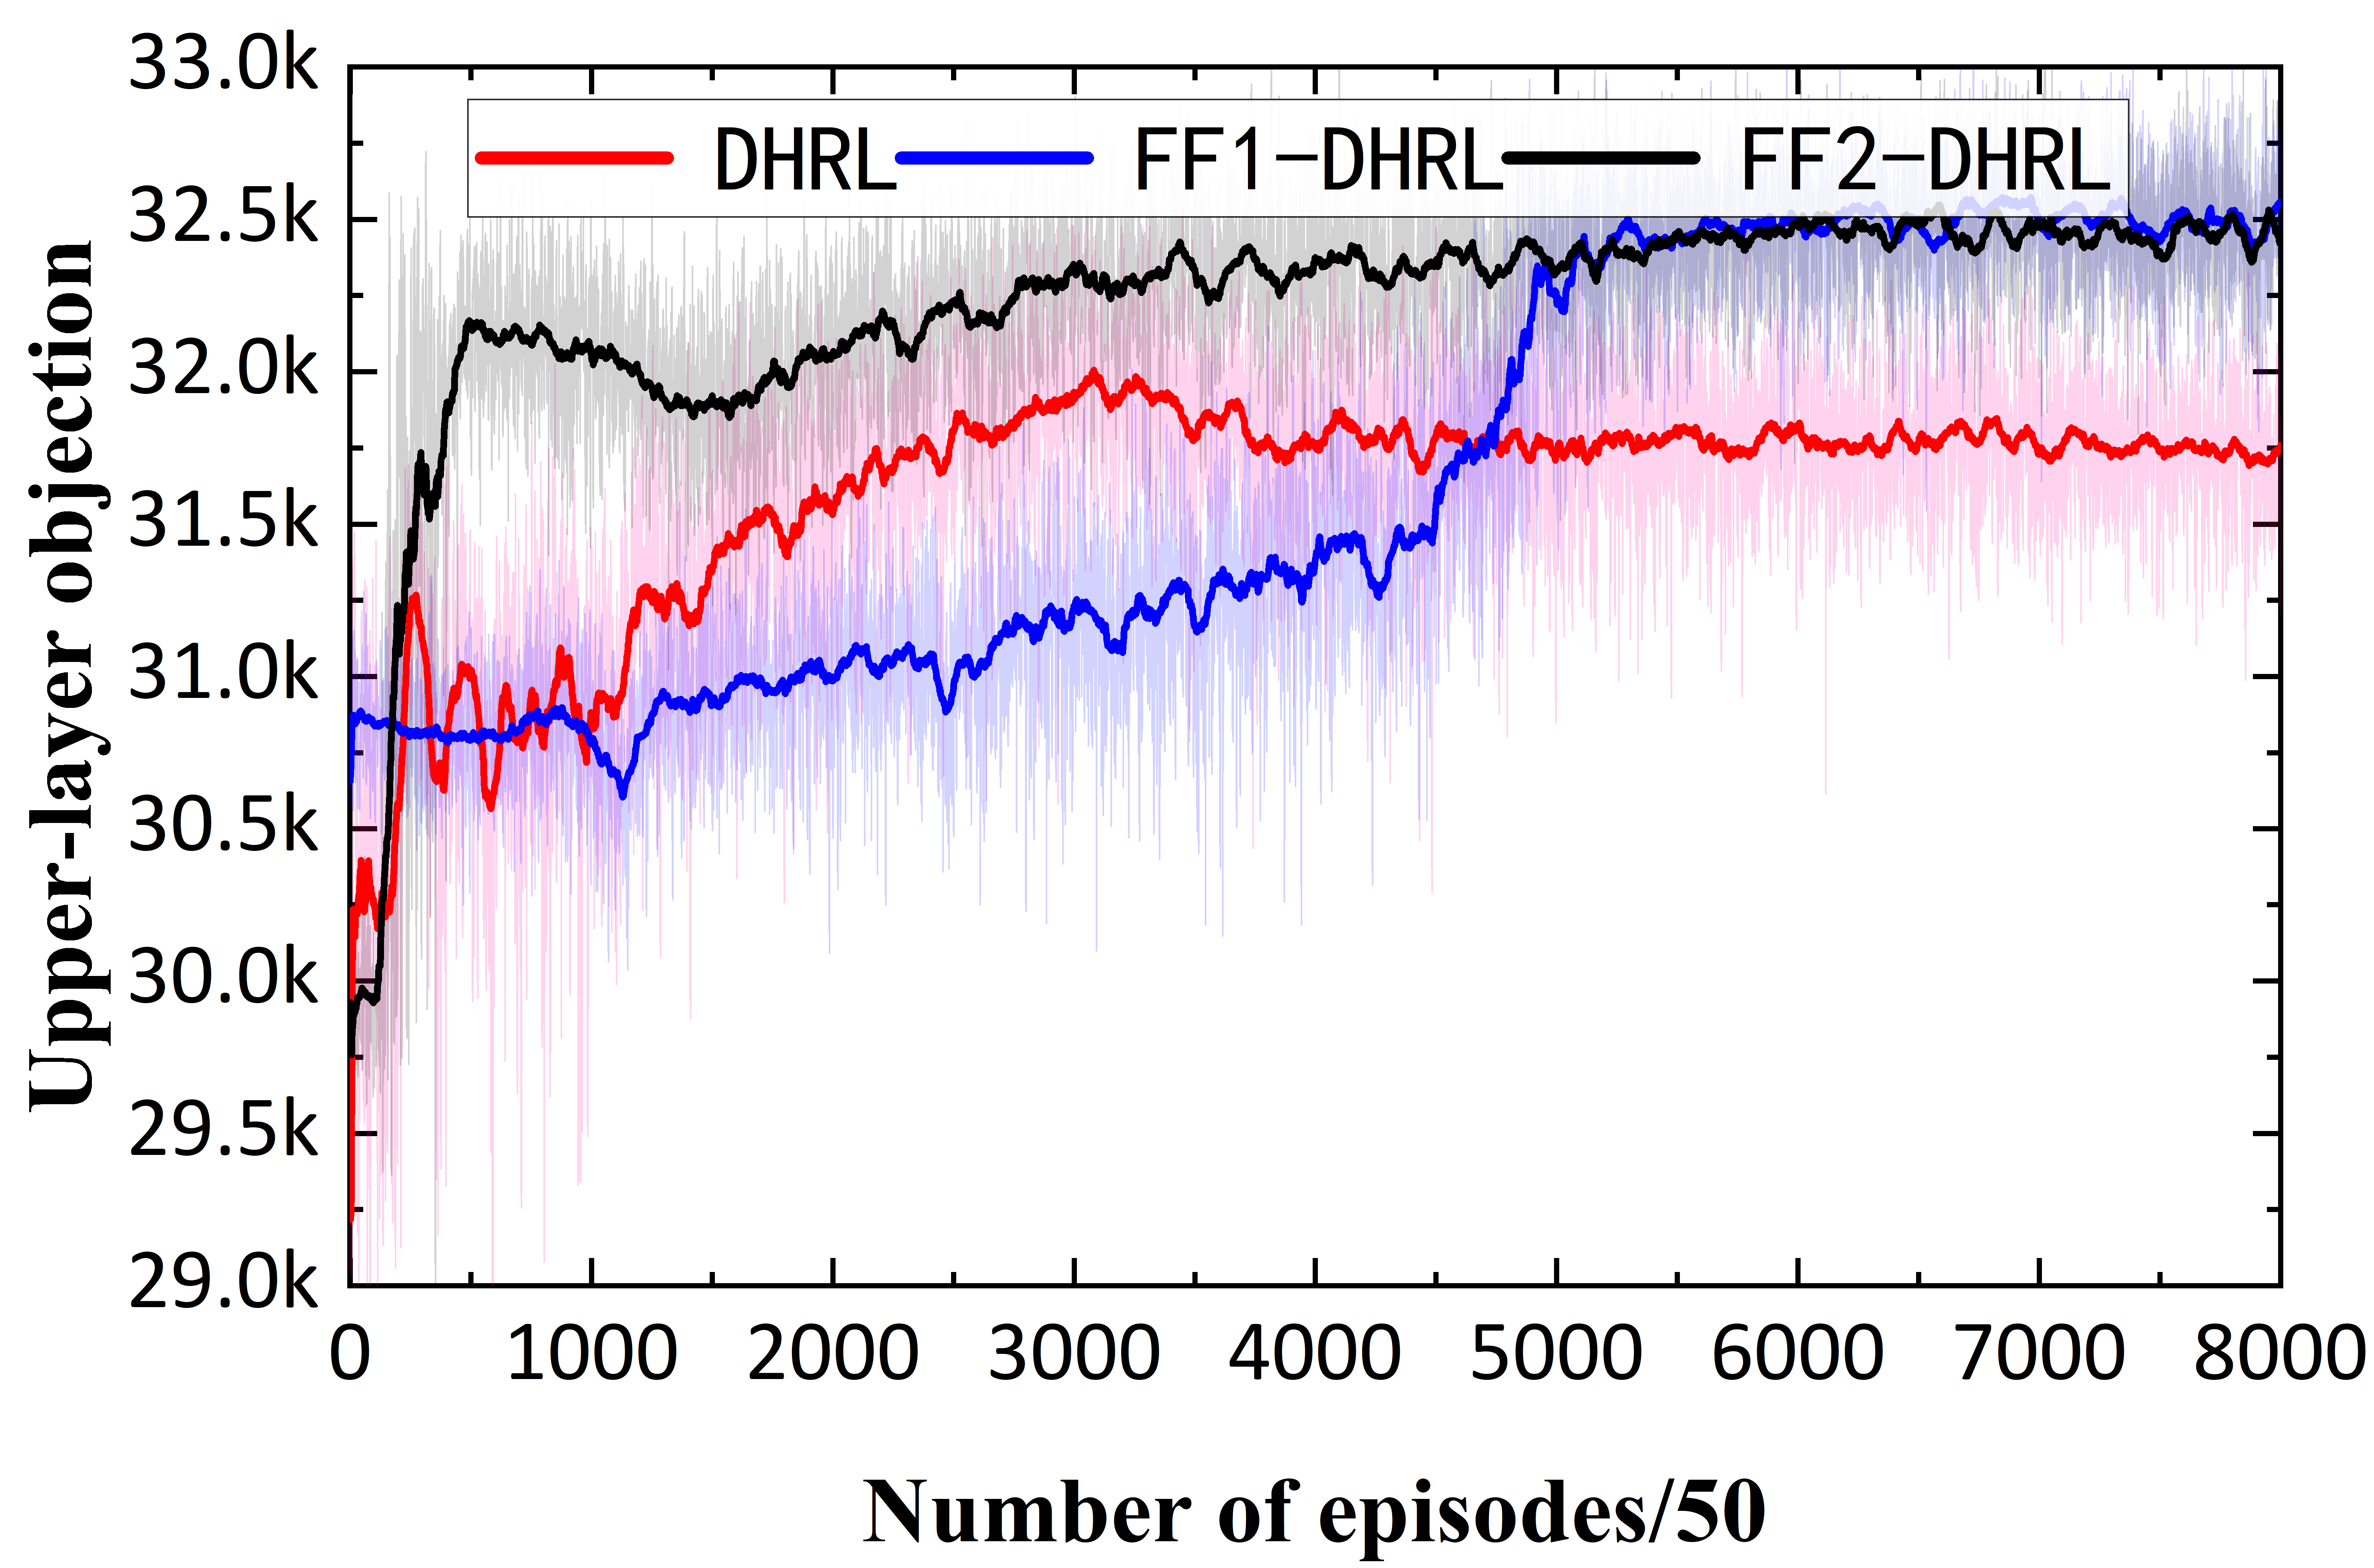
\includegraphics[width=0.49\columnwidth]{figures/LearningCurves_goal_upper}
\par\end{centering}
}\subfloat[Lower-layer objection]{\begin{centering}
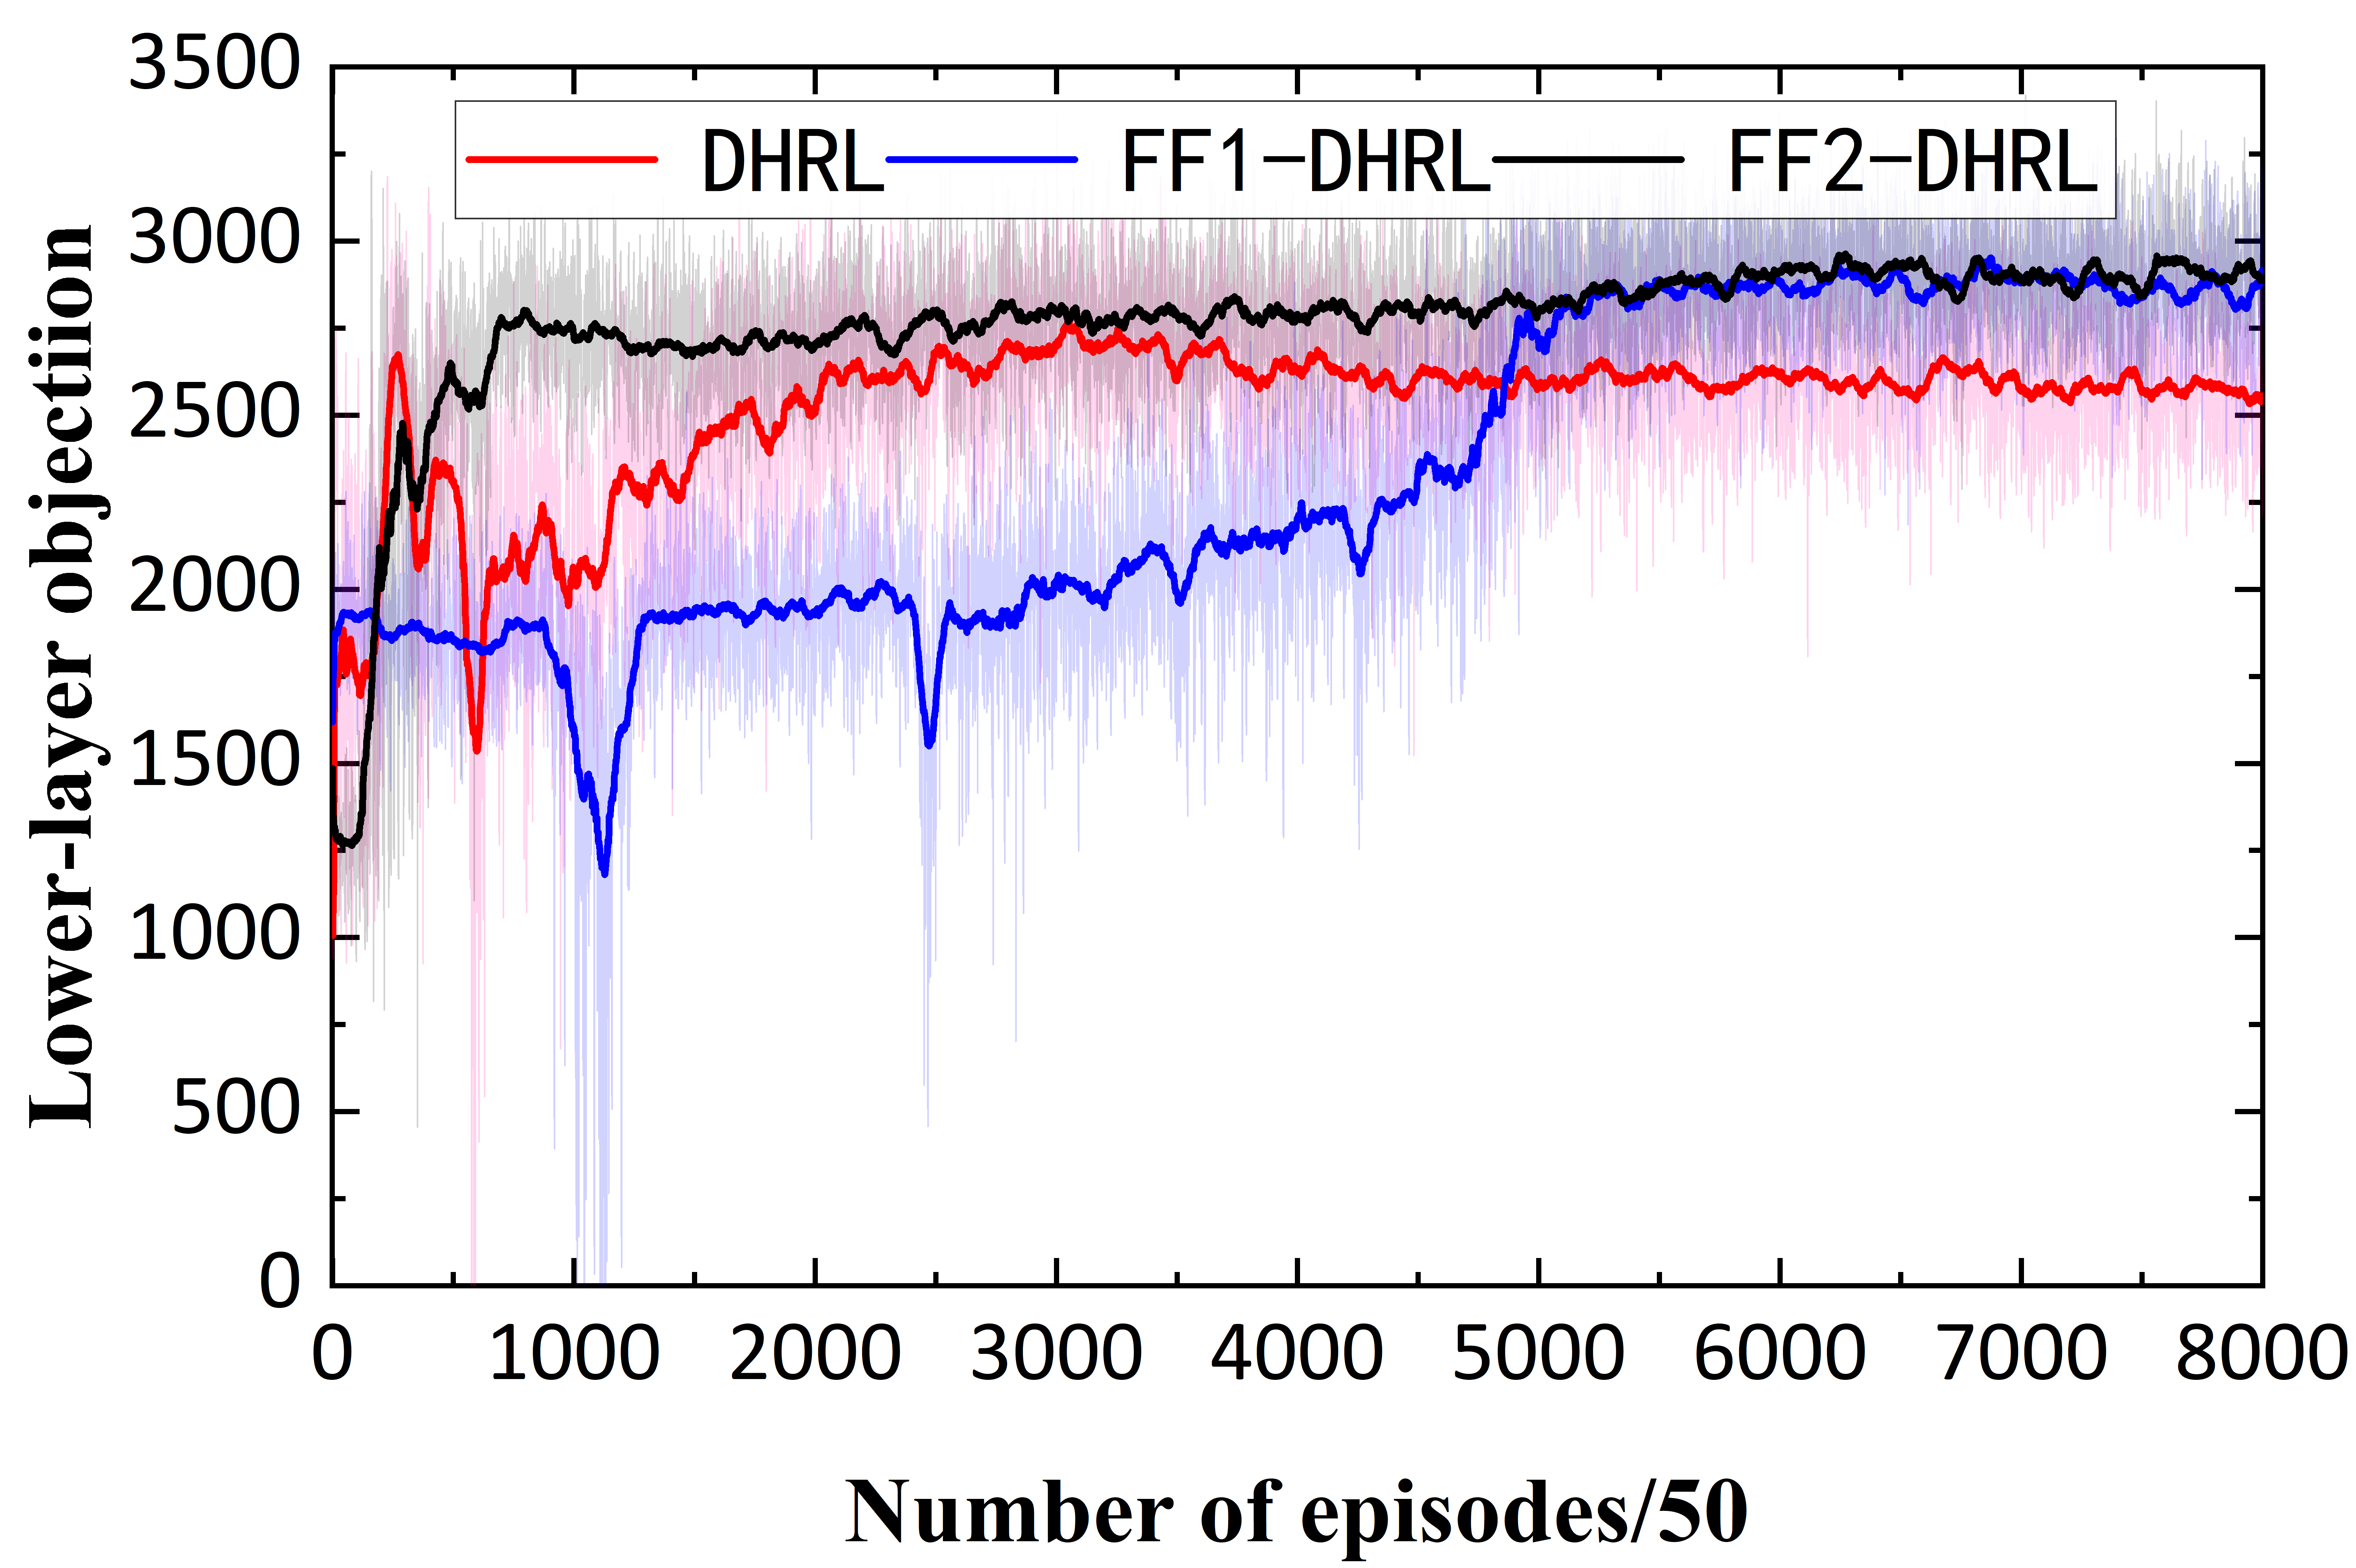
\includegraphics[width=0.49\columnwidth]{figures/LearningCurves_goal_lower}
\par\end{centering}
}
\par\end{centering}
\begin{centering}
\subfloat[Revenue derived from DR]{\begin{centering}
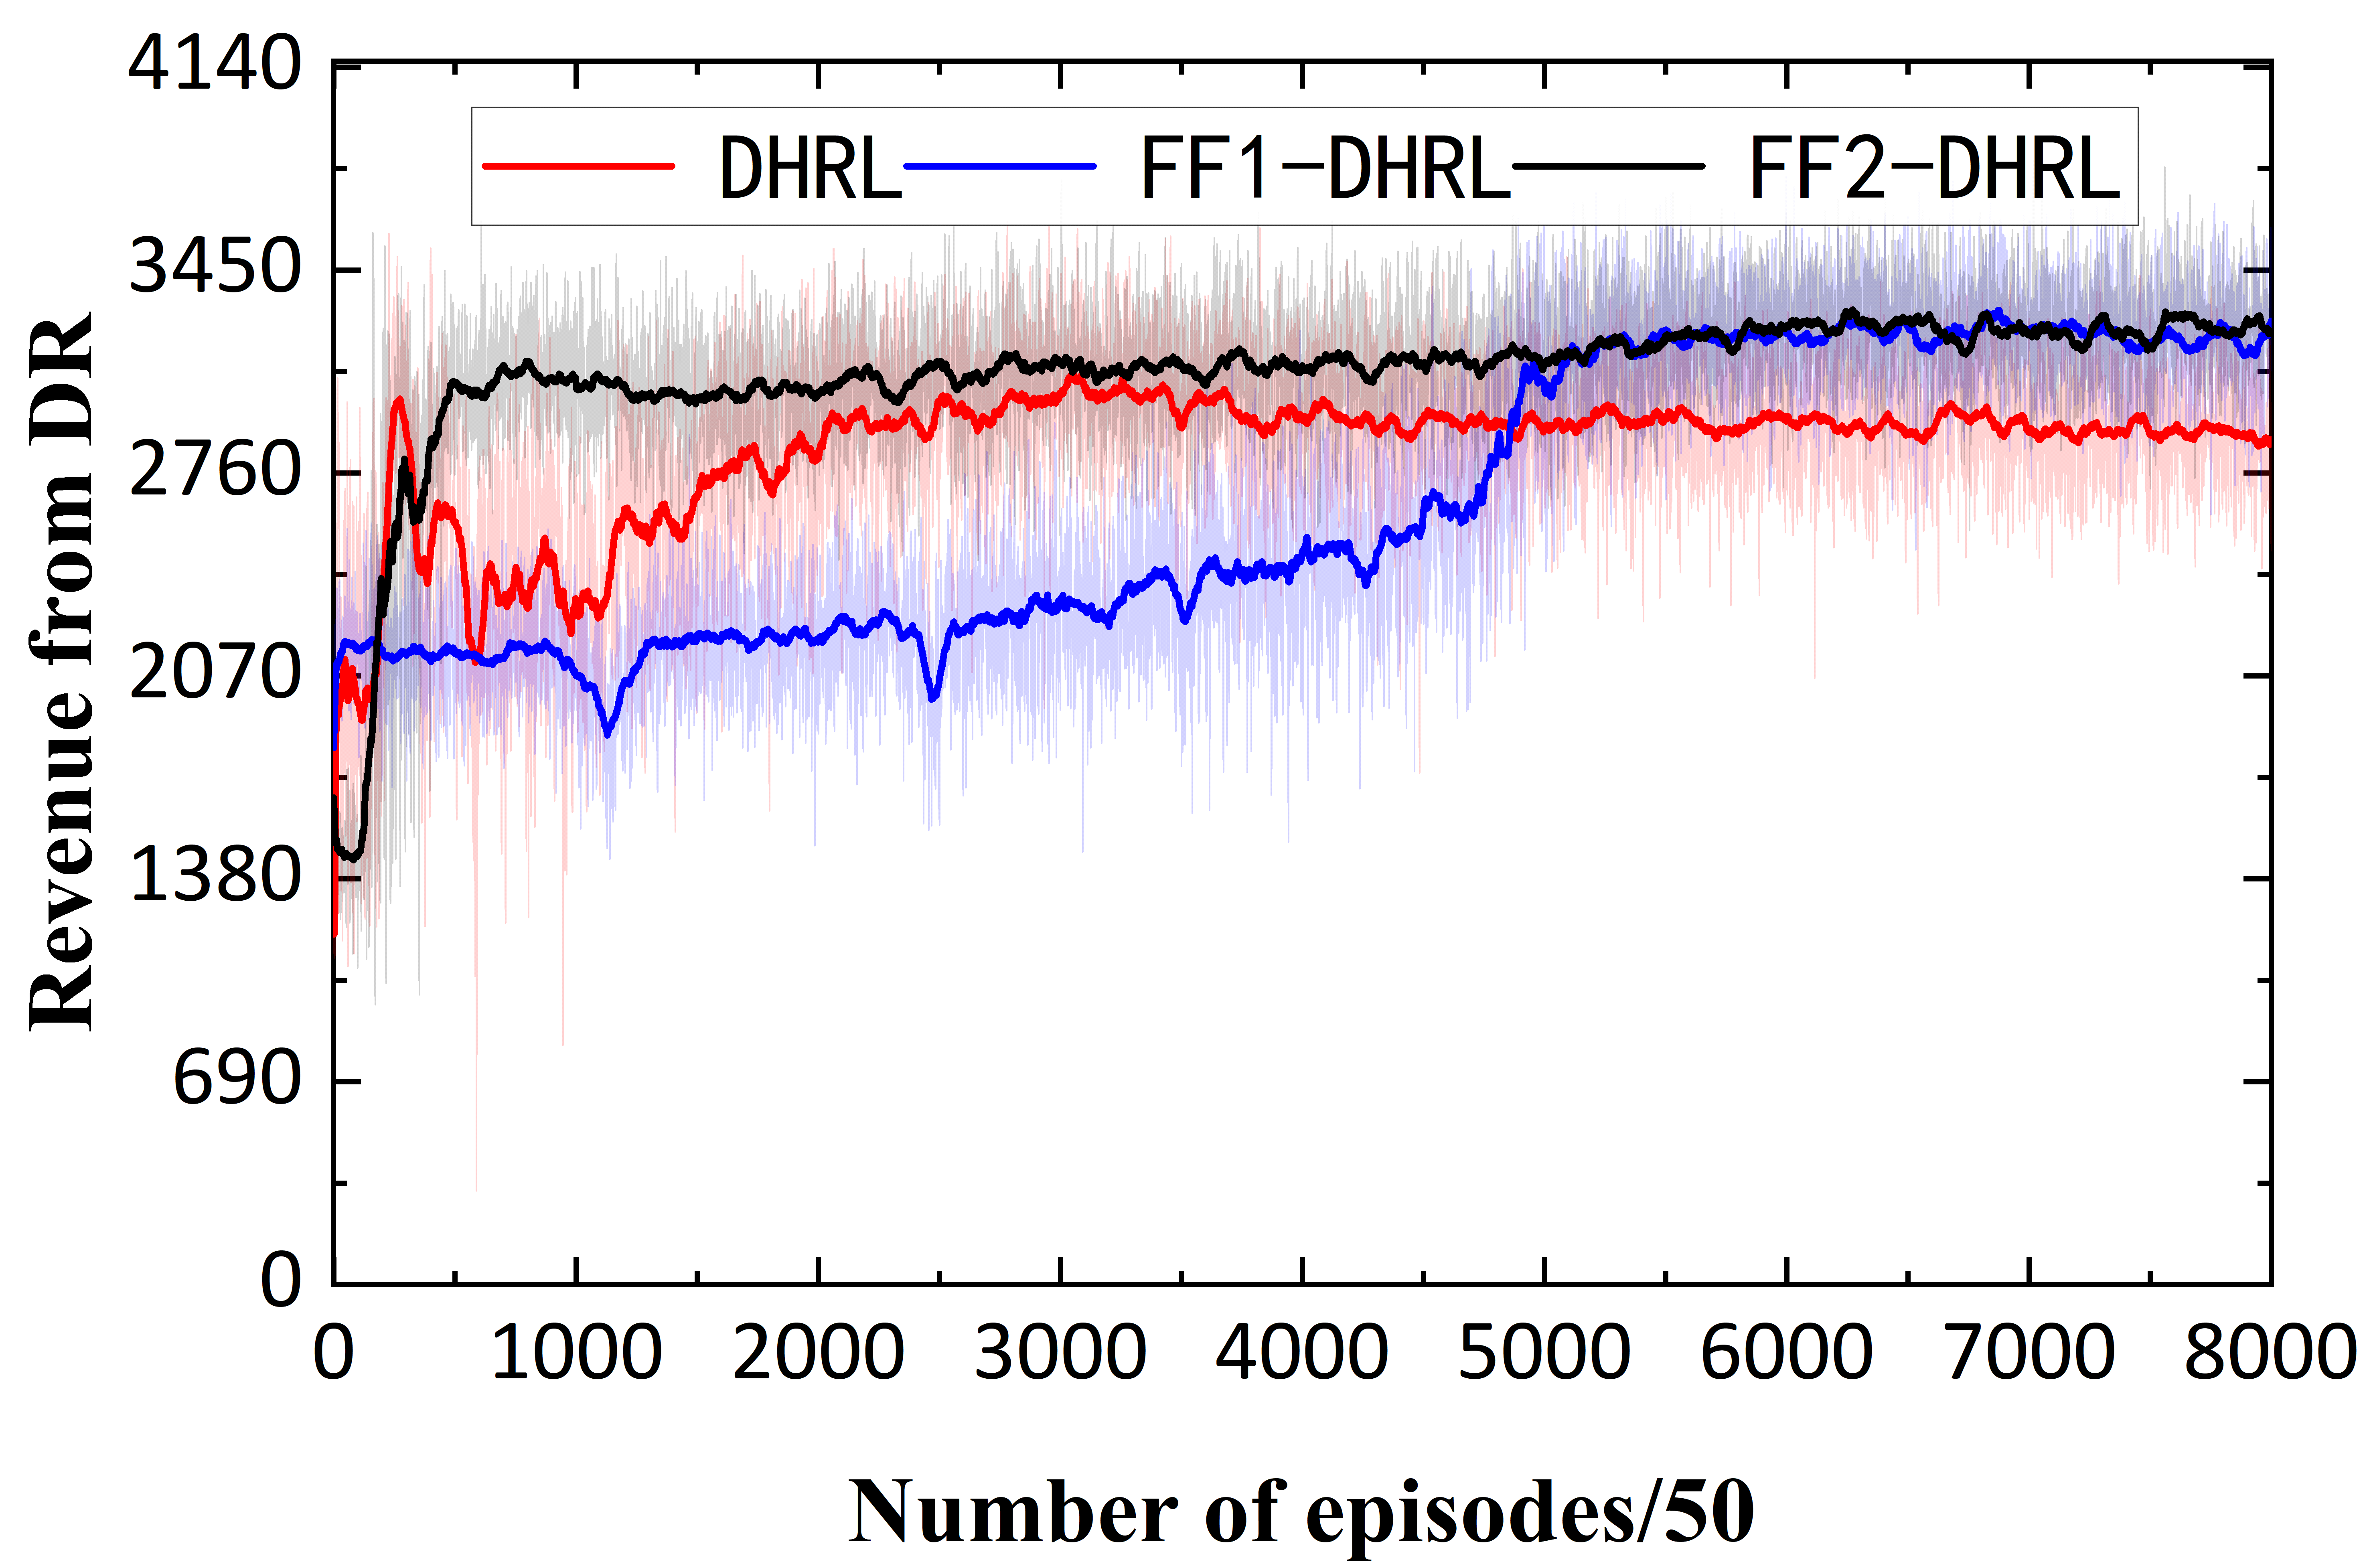
\includegraphics[width=0.49\columnwidth]{figures/LearningCurves_DR}
\par\end{centering}
}\subfloat[User satisfaction cost]{\begin{centering}
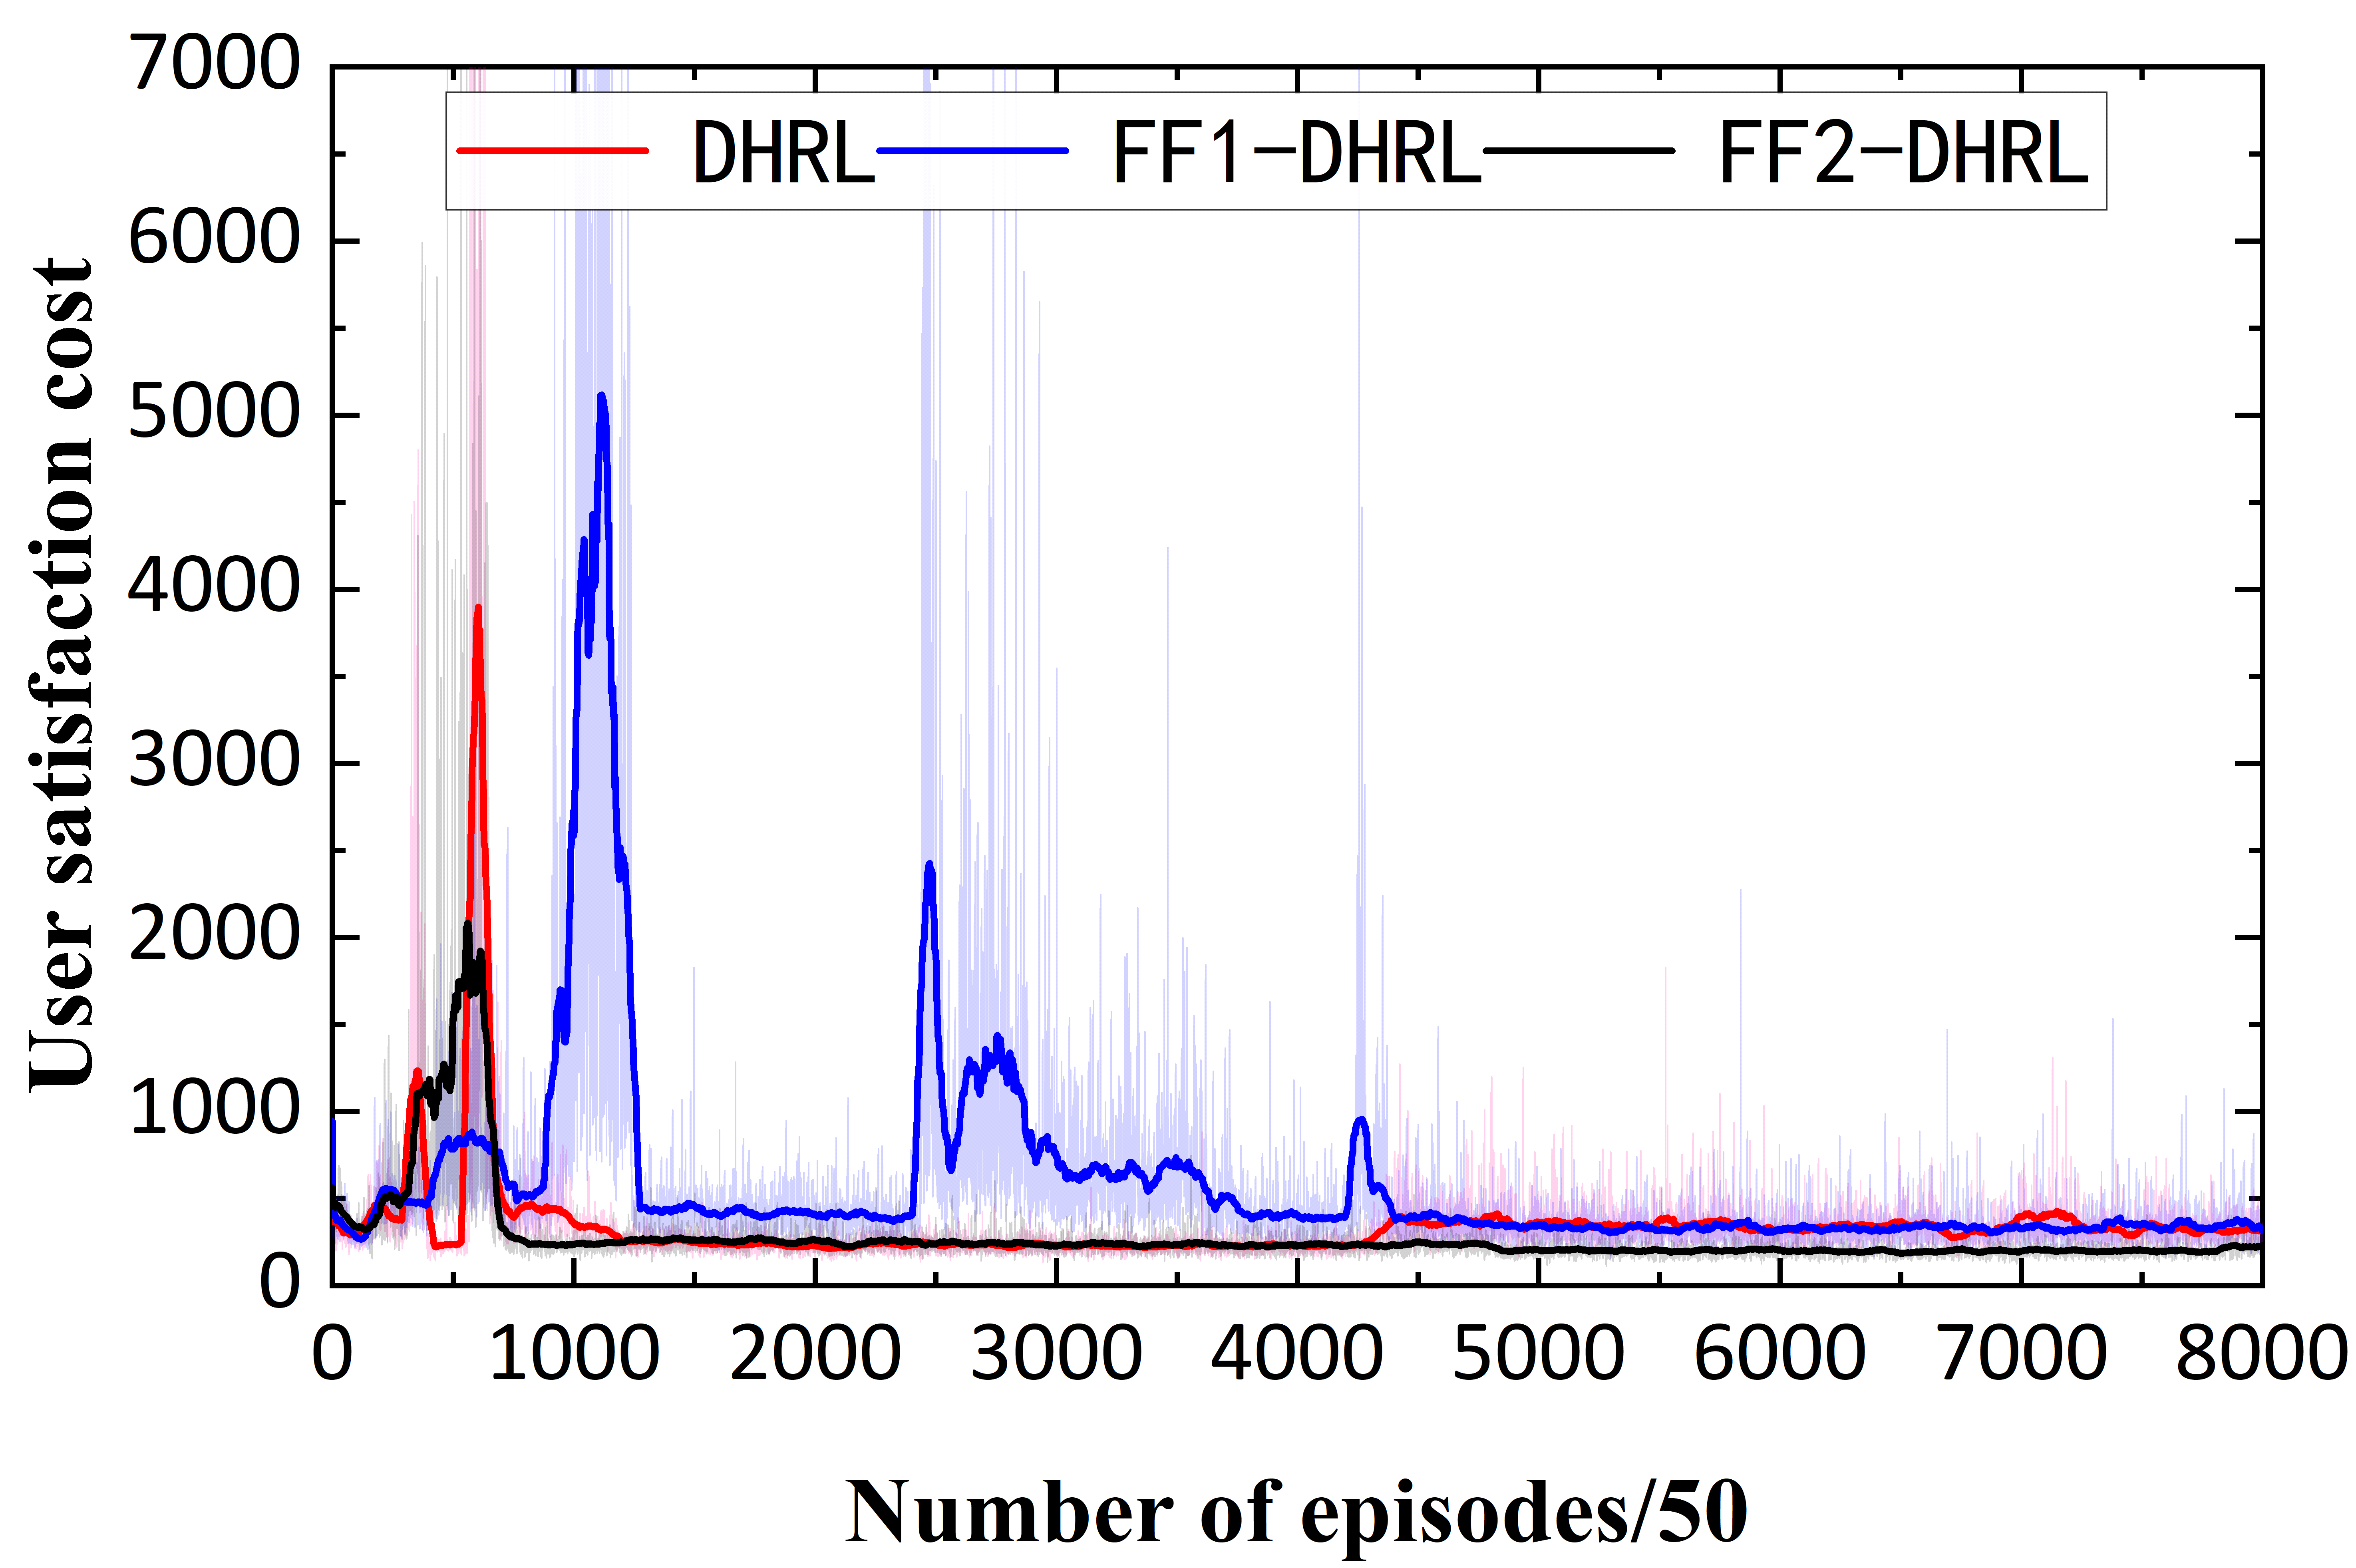
\includegraphics[width=0.49\columnwidth]{figures/LearningCurves_QoS}
\par\end{centering}
}
\par\end{centering}
\centering{}
\caption{Learning curves of three algorithms.The red, blue curves and black curves are the learning curves of DHRL, FF1-DHRL and FF2-DHRL, respectively.}
\label{fig:Learning-curves}
\end{figure}


% \begin{figure}[htbp]
%     \centering
%     \includegraphics[width=1\linewidth]{figures/response_power.png}
%     \caption{The response power curves of charging stations under the optimized strategy obtained by using DHRL, FF1-DHRL and FF2-DHRL, respectively.}
%     \label{fig:DR_curves}
% \end{figure}

% \begin{figure}[htbp]
%     \centering
%     \includegraphics[width=1\linewidth]{figures/ele_dr.png}
%     \caption{The difference in electricity consumption between the original strategy and the optimized strategy derived from DHRL, FF1-DHRL and FF2-DHRL, respectively.}
%     \label{fig:DR_electricity}
% \end{figure}


Fig. \ref{fig:Learning-curves} presents learning curves of the three methods.  It is evident that both the standard DHRL and its enhanced versions demonstrate robust convergence.  Notably, DHRL integrated with FF surpasses the basic DHRL in terms of convergence speed.  This superiority likely results from FF's ability to minimize the impact of redundant or weakly correlated states from EVs in charging piles and waiting queues on decision-making.  FF sharpens the agent's focus on pivotal decision-related information.  In the context of dual-layer collaborative optimization, enhancing the input state of the upper-layer agent with FF has led to improvements in the optimization objectives for both upper and lower-layer agents, outperforming the conventional DHRL approach.  Additionally, when comparing FF1-DHRL and FF2-DHRL, it is observed that different fusion states influence the learning trajectory.  The fusion state applied in this study accelerates the learning process more effectively than FF1-DHRL, possibly due to FF2's refined encapsulation of crucial information. 
% It can be observed that, regardless of whether feature fusion
% is adopted, DHRL and the improved DHRLs exhibit good convergence performance.
% However, when comparing the optimization objective values after convergence,
% it can be observed that the DHRL with FF outperforms the unimproved
% DHRL in terms of performance. This might be attributed to the fact
% that adopting FF can reduce the influence of some redundant or weakly
% correlated states of EVs in the charging piles and waiting queues
% on the agent's decision-making. This enhances the agent's perception
% of key information related to the decision-making problem. It's worth
% noting that in the dual-layer collaborative optimization, even though
% we only fuse information for the input state of the upper-layer agent,
% the optimization objectives for both the upper and lower-layer agents
% have improved compared to the traditional DHRL. Further comparing
% FF1-DHRL and FF2-DHRL, we can analyze that adopting different fusion
% states will introduce variations in the learning process. The method
% with the fusion state proposed in this paper exhibits a noticeably
% faster learning rate than FF1-DHRL. This might be because FF2 offers
% a more concentrated representation of key information.


Fig. \ref{fig:DR_curves} and \ref{fig:DR_electricity} illustrate the effectiveness of three optimization strategies in peak shaving and valley filling.  In periods of low power grid demand, the SPM reduces service prices, increasing the arrival rate of EVs and thereby enhancing charging service revenue.  Conversely, during times of tight power supply, such as periods of peak electricity price, the SPM raises service prices to discourage EV charging, effectively reducing the load on charging stations.  Additionally, during peak-shaving periods  $\phi_\textrm{ps}^{1}$ and $\phi_\textrm{ps}^{2}$, if the power grid demands load reduction and the station's current load is excessive, the CPC issues power adjustment commands to the charging piles based on the station's operational status. This action further aligns with the peak adjustment requirements of the higher-level dispatching authority. 

% When the power grid supply demand is loose, the SPM lowers the service
% electricity price to increase the arrival rate of EVs, thereby enhancing
% the revenue from charging services. During times of tight power supply,
% such as during peak electricity price periods, the SPM raises the
% service electricity price to reduce the charging intentions of EV
% users, achieving a reduction in the load of charging stations during
% peak electricity usage periods of the grid. Meanwhile, during the
% peak shaving periods $\phi_{ps}^{1}$ and $\phi_{ps}^{2}$, if the
% power grid issues power reduction commands and the current load of
% the station is still too high, the CPC will issue power adjustment
% commands to the charging piles based on the station current operating
% point, further meeting the peak adjustment demands of the higher-level
% dispatching organization.

\begin{figure}[h]
  \centering
  % 第一张子图
  \subfloat[Response power curves]{
    \includegraphics[width=0.45\linewidth]{figures/response_power.png}
    \label{fig:DR_curves}
  }
  \hfill % 在两张图片之间添加一些空间
  % 第二张子图
  \subfloat[Response electricity]{
    \includegraphics[width=0.45\linewidth]{figures/ele_dr.png}
    \label{fig:DR_electricity}
  }
  \caption{The response results of charging stations under the optimized strategy obtained by using DHRL, FF1-DHRL and FF2-DHRL, respectively.}
\end{figure}

Table \ref{tab:Statistical-revenues} details the performance of the three optimization strategies.  Economically, the FF2-DHRL approach excels, surpassing others in revenue generation from grid demand response and profits from EV charging services.  Further, an analysis of electricity consumption patterns under peak, float, and valley price periods reveals that FF2-DHRL most effectively achieves peak shaving and valley filling.  This success can be attributed to its upper-layer agent setting more appropriate service prices than its counterparts.  These results also serve as indirect validations of the proposed feature fusion technique's efficacy in enhancing the algorithm. 
% it is found that the FF2-DHRL method outperforms others in both revenue
% gained from participating in grid demand response and profit earned
% from providing charging services to EV users. Additionally, by examining
% the electricity consumption of the three strategies during periods
% of peak, float, and valley electricity prices, it is apparent that
% the FF2-DHRL method achieves the most optimal peak shaving and valley
% filling effect. The reason for this outcome is that the service electricity
% prices set by the upper-level agent of the FF2-DHRL method are more
% reasonable compared to the other two methods. This also indirectly
% validates the effectiveness of the feature fusion method we proposed
% for improving the algorithm.
%% tab:Statistical-revenues
% \begin{table}[htbp]
% \caption{Statistical revenues of the three methods}
% \label{tab:Statistical-revenues}
% \centering
% \begin{tabular*}{0.98\linewidth}{@{\extracolsep{\fill}}>{\centering}p{0.1\textwidth}>{\raggedleft}p{0.08\textwidth}>{\raggedleft}p{0.08\textwidth}>{\raggedleft}p{0.08\textwidth}>{\centering}p{0.15\textwidth}>{\centering}p{0.18\textwidth}}
% \toprule
% \multirow{2}{0.1\textwidth}{Methods} & \multicolumn{3}{c}{Electric Consumption (\kwh)} & \multirow{2}{0.15\textwidth}{Peak Shaving Benefits (\$)} & \multirow{2}{0.23\textwidth}{Revenue from Charging Services (\$)} \tabularnewline
% \cmidrule{2-4}
%  & $T_{peak}$ & $T_{float}$ & $T_{valley}$ &  & \tabularnewline
% \midrule
% DHRL & 10562 & 7495 & 10762 & 1714 & 28496 \tabularnewline
% FF1-DHRL & 10558 & 7484 & 10828 & 1437 & 28283 \tabularnewline
% FF2-DHRL & 9989 & 7417 & 12115 & 2644 & 28608 \tabularnewline
% \bottomrule
% \end{tabular*}
% \end{table}

\begin{table}[htbp]
\caption{Statistical revenues of the three methods}
\label{tab:Statistical-revenues}
\centering
\begin{tabular*}{0.98\linewidth}{@{\extracolsep{\fill}}>{\centering}m{0.1\textwidth}>{\raggedleft}m{0.08\textwidth}>{\raggedleft}m{0.08\textwidth}>{\raggedleft}m{0.08\textwidth}>{\centering}m{0.15\textwidth}>{\centering}m{0.18\textwidth}}
\toprule
\multirow{2}{0.09\textwidth}{Methods} & \multicolumn{3}{c}{Electric Consumption (\kwh)} & \multirow{2}{0.15\textwidth}{Peak-shaving Benefits (\$)} & \multirow{2}{0.24\textwidth}{Revenue of Charging Services (\$)} \tabularnewline
\cmidrule{2-4}
 & $T_{peak}$ & $T_{float}$ & $T_{valley}$ &  & \tabularnewline
\midrule
DHRL & 10562 & 7495 & 10762 & 1714 & 28496 \tabularnewline
FF1-DHRL & 10558 & 7484 & 10828 & 1437 & 28283 \tabularnewline
FF2-DHRL & 9989 & 7417 & 12115 & 2644 & 28608 \tabularnewline
\bottomrule
\end{tabular*}
\end{table}


% \begin{table*}[tp]
% \caption{\label{tab:Statistical-revenues}Statistical revenues of the three
% methods}
% \noindent \centering{}%
% \begin{tabular*}{0.98\linewidth}{@{\extracolsep{\fill}}>{\centering}p{0.1\textwidth}>{\raggedleft}p{0.08\textwidth}>{\raggedleft}p{0.08\textwidth}>{\raggedleft}p{0.08\textwidth}>{\centering}p{0.15\textwidth}>{\centering}p{0.18\textwidth}}
% \toprule
% \multirow{2}{0.1\textwidth}{\noindent \centering{}Methods} & \multicolumn{3}{c}{Electric Consumption\kwh} & \multirow{2}{0.15\textwidth}{\noindent \centering{}Peak Shaving Benefits (\$)} & \multirow{2}{0.18\textwidth}{\noindent \centering{}Revenue from Charging Services (\$)}\tabularnewline
% \cmidrule{2-4} \cmidrule{3-4} \cmidrule{4-4}
%  & \noindent \centering{}$\mathbf{T_{peak}}$ & \noindent \centering{}$\mathbf{T_{float}}$ & \noindent \centering{}$\mathbf{T_{valley}}$ &  & \tabularnewline
% \midrule
% \noindent \centering{}DHRL & \noindent \centering{}10562 & \noindent \centering{}7495 & \noindent \centering{}10762 & \noindent \centering{}1714 & \noindent \centering{}28496\tabularnewline
% \noindent \centering{}FF1-DHRL & \noindent \centering{}10558 & \noindent \centering{}7484 & \noindent \centering{}10828 & \noindent \centering{}1437 & \noindent \centering{}28283\tabularnewline
% \noindent \centering{}FF2-DHRL & \noindent \centering{}9989 & \noindent \centering{}7417 & \noindent \centering{}12115 & \noindent \centering{}2644 & \noindent \centering{}28608\tabularnewline
% \bottomrule
% \end{tabular*}
% \end{table*}

\begin{figure}[htbp]
\begin{centering}
\subfloat[\emph{Sch-\mbox{II}.}]{\begin{centering}
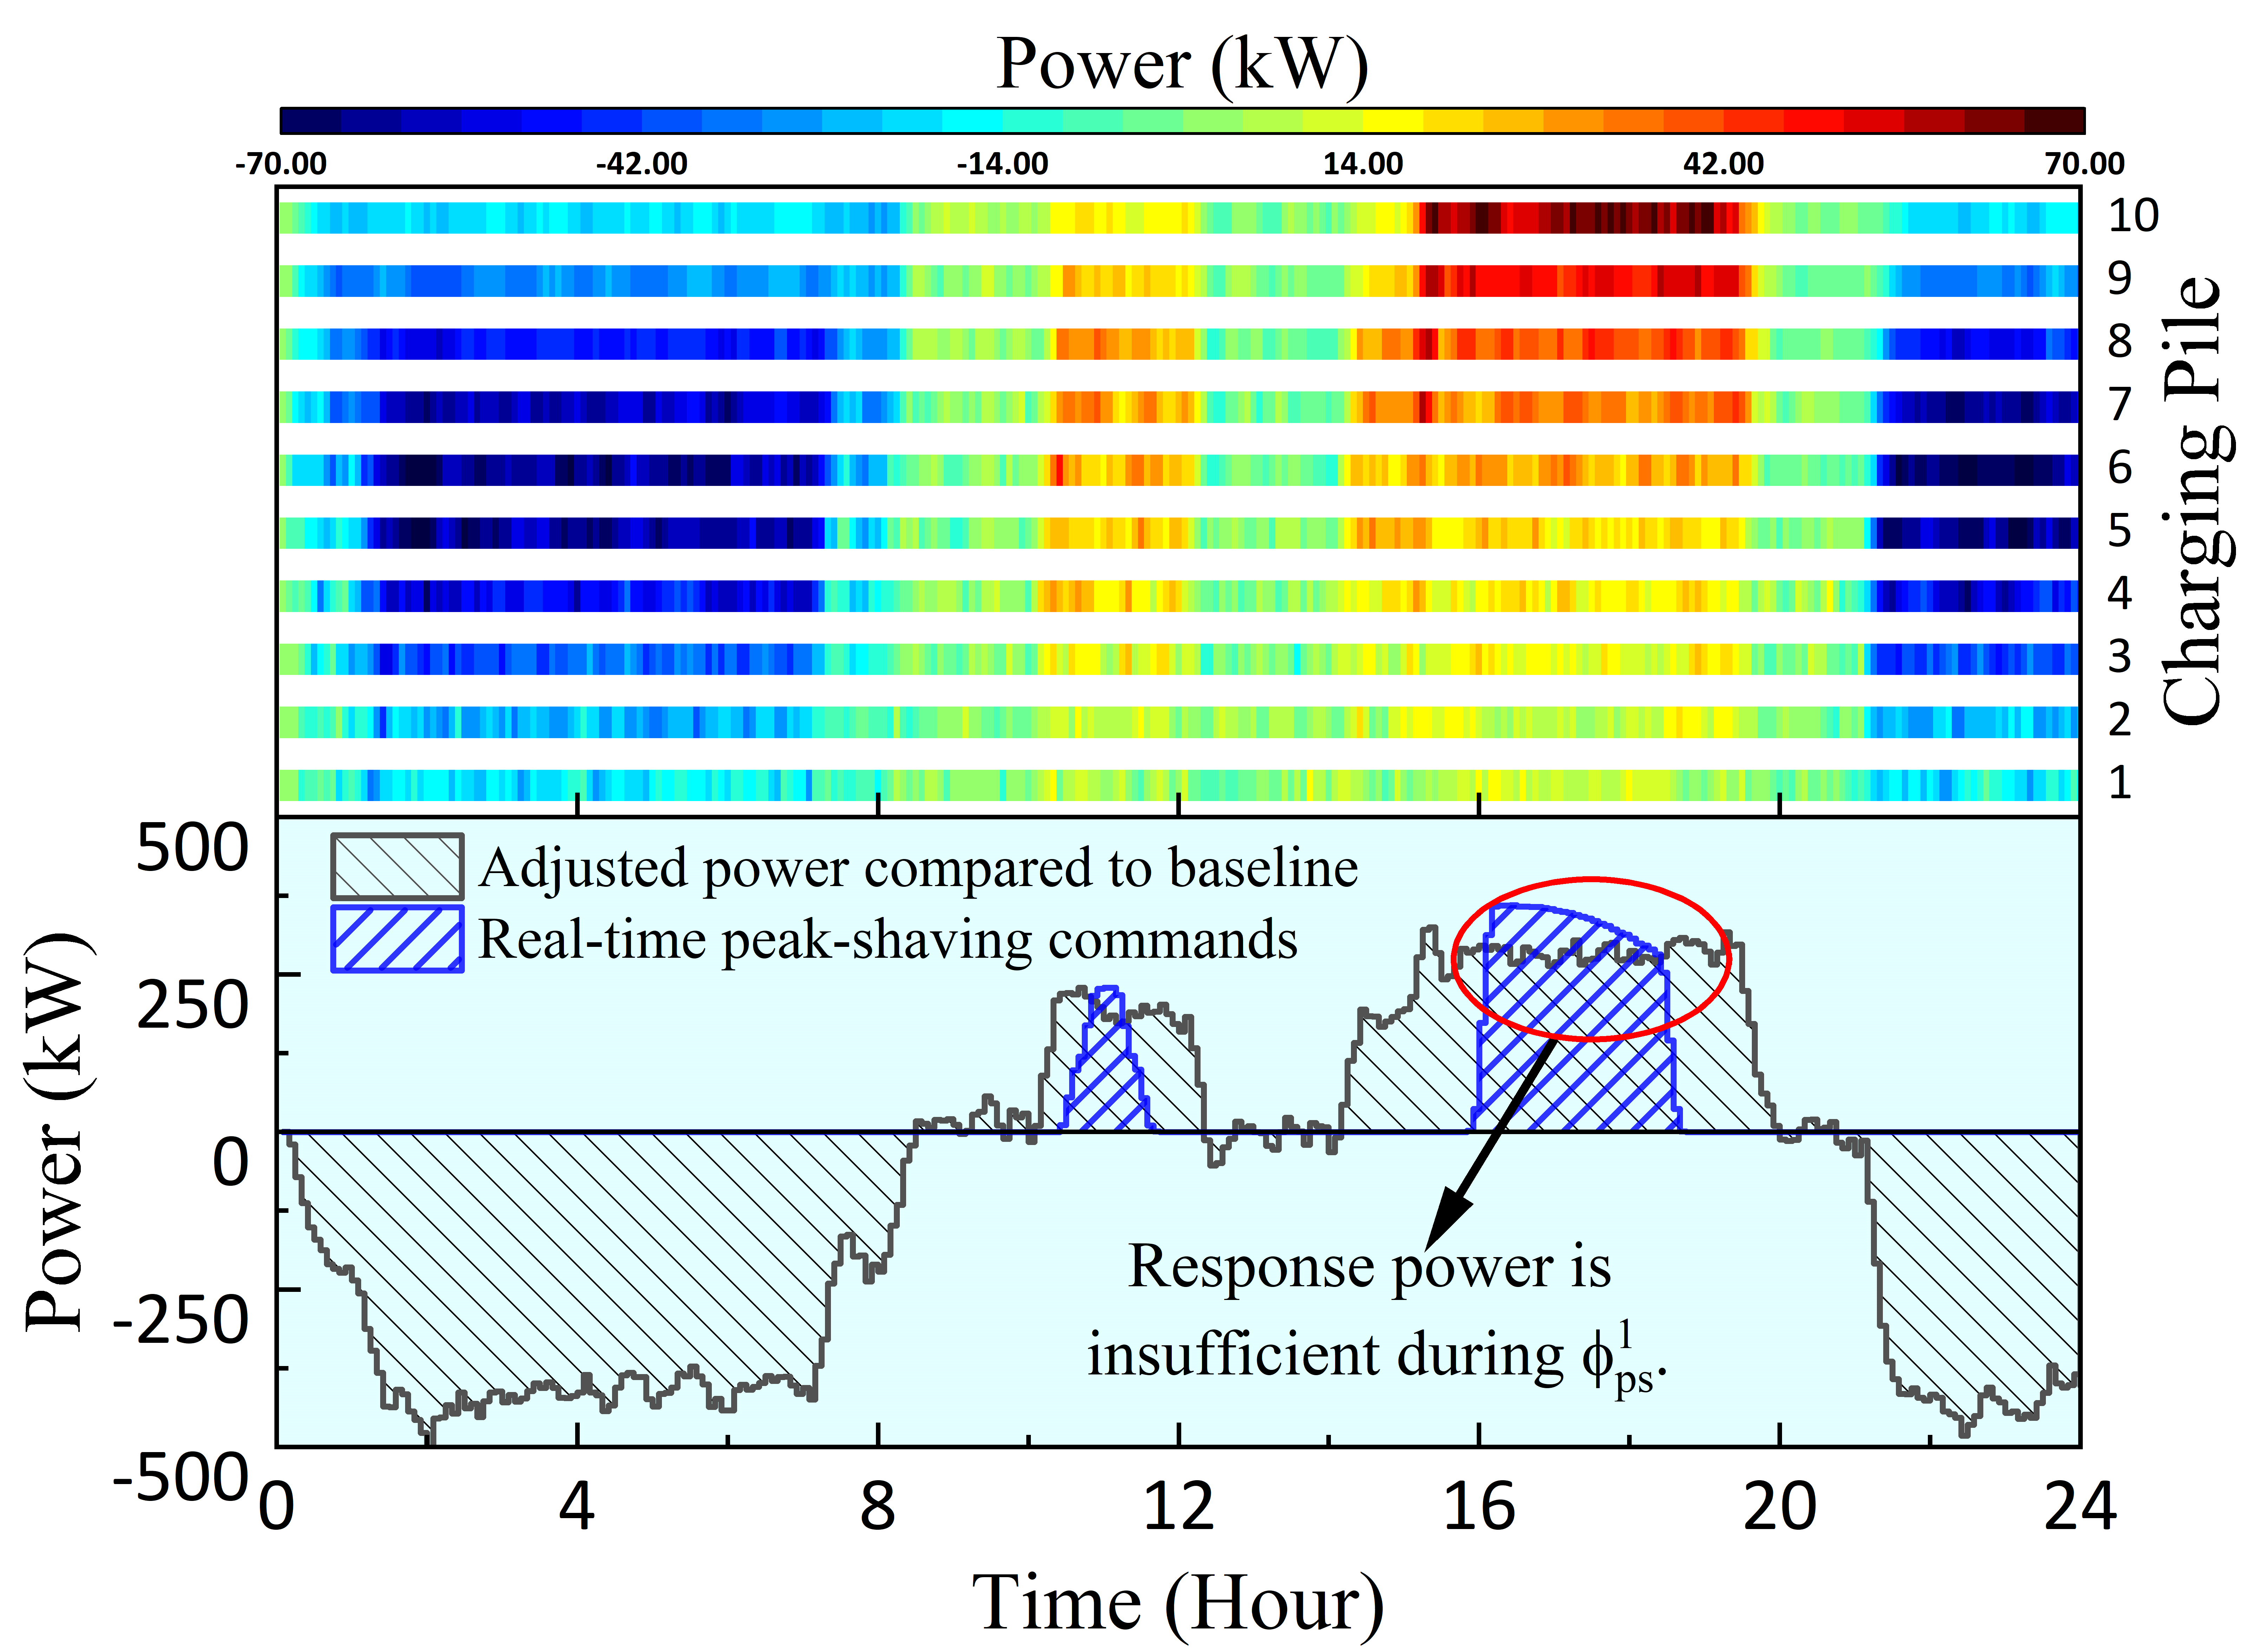
\includegraphics[width=0.49\linewidth]{figures/sch2_heatmap}
\par\end{centering}
}\subfloat[\emph{Sch-\mbox{III}.}]{\centering{}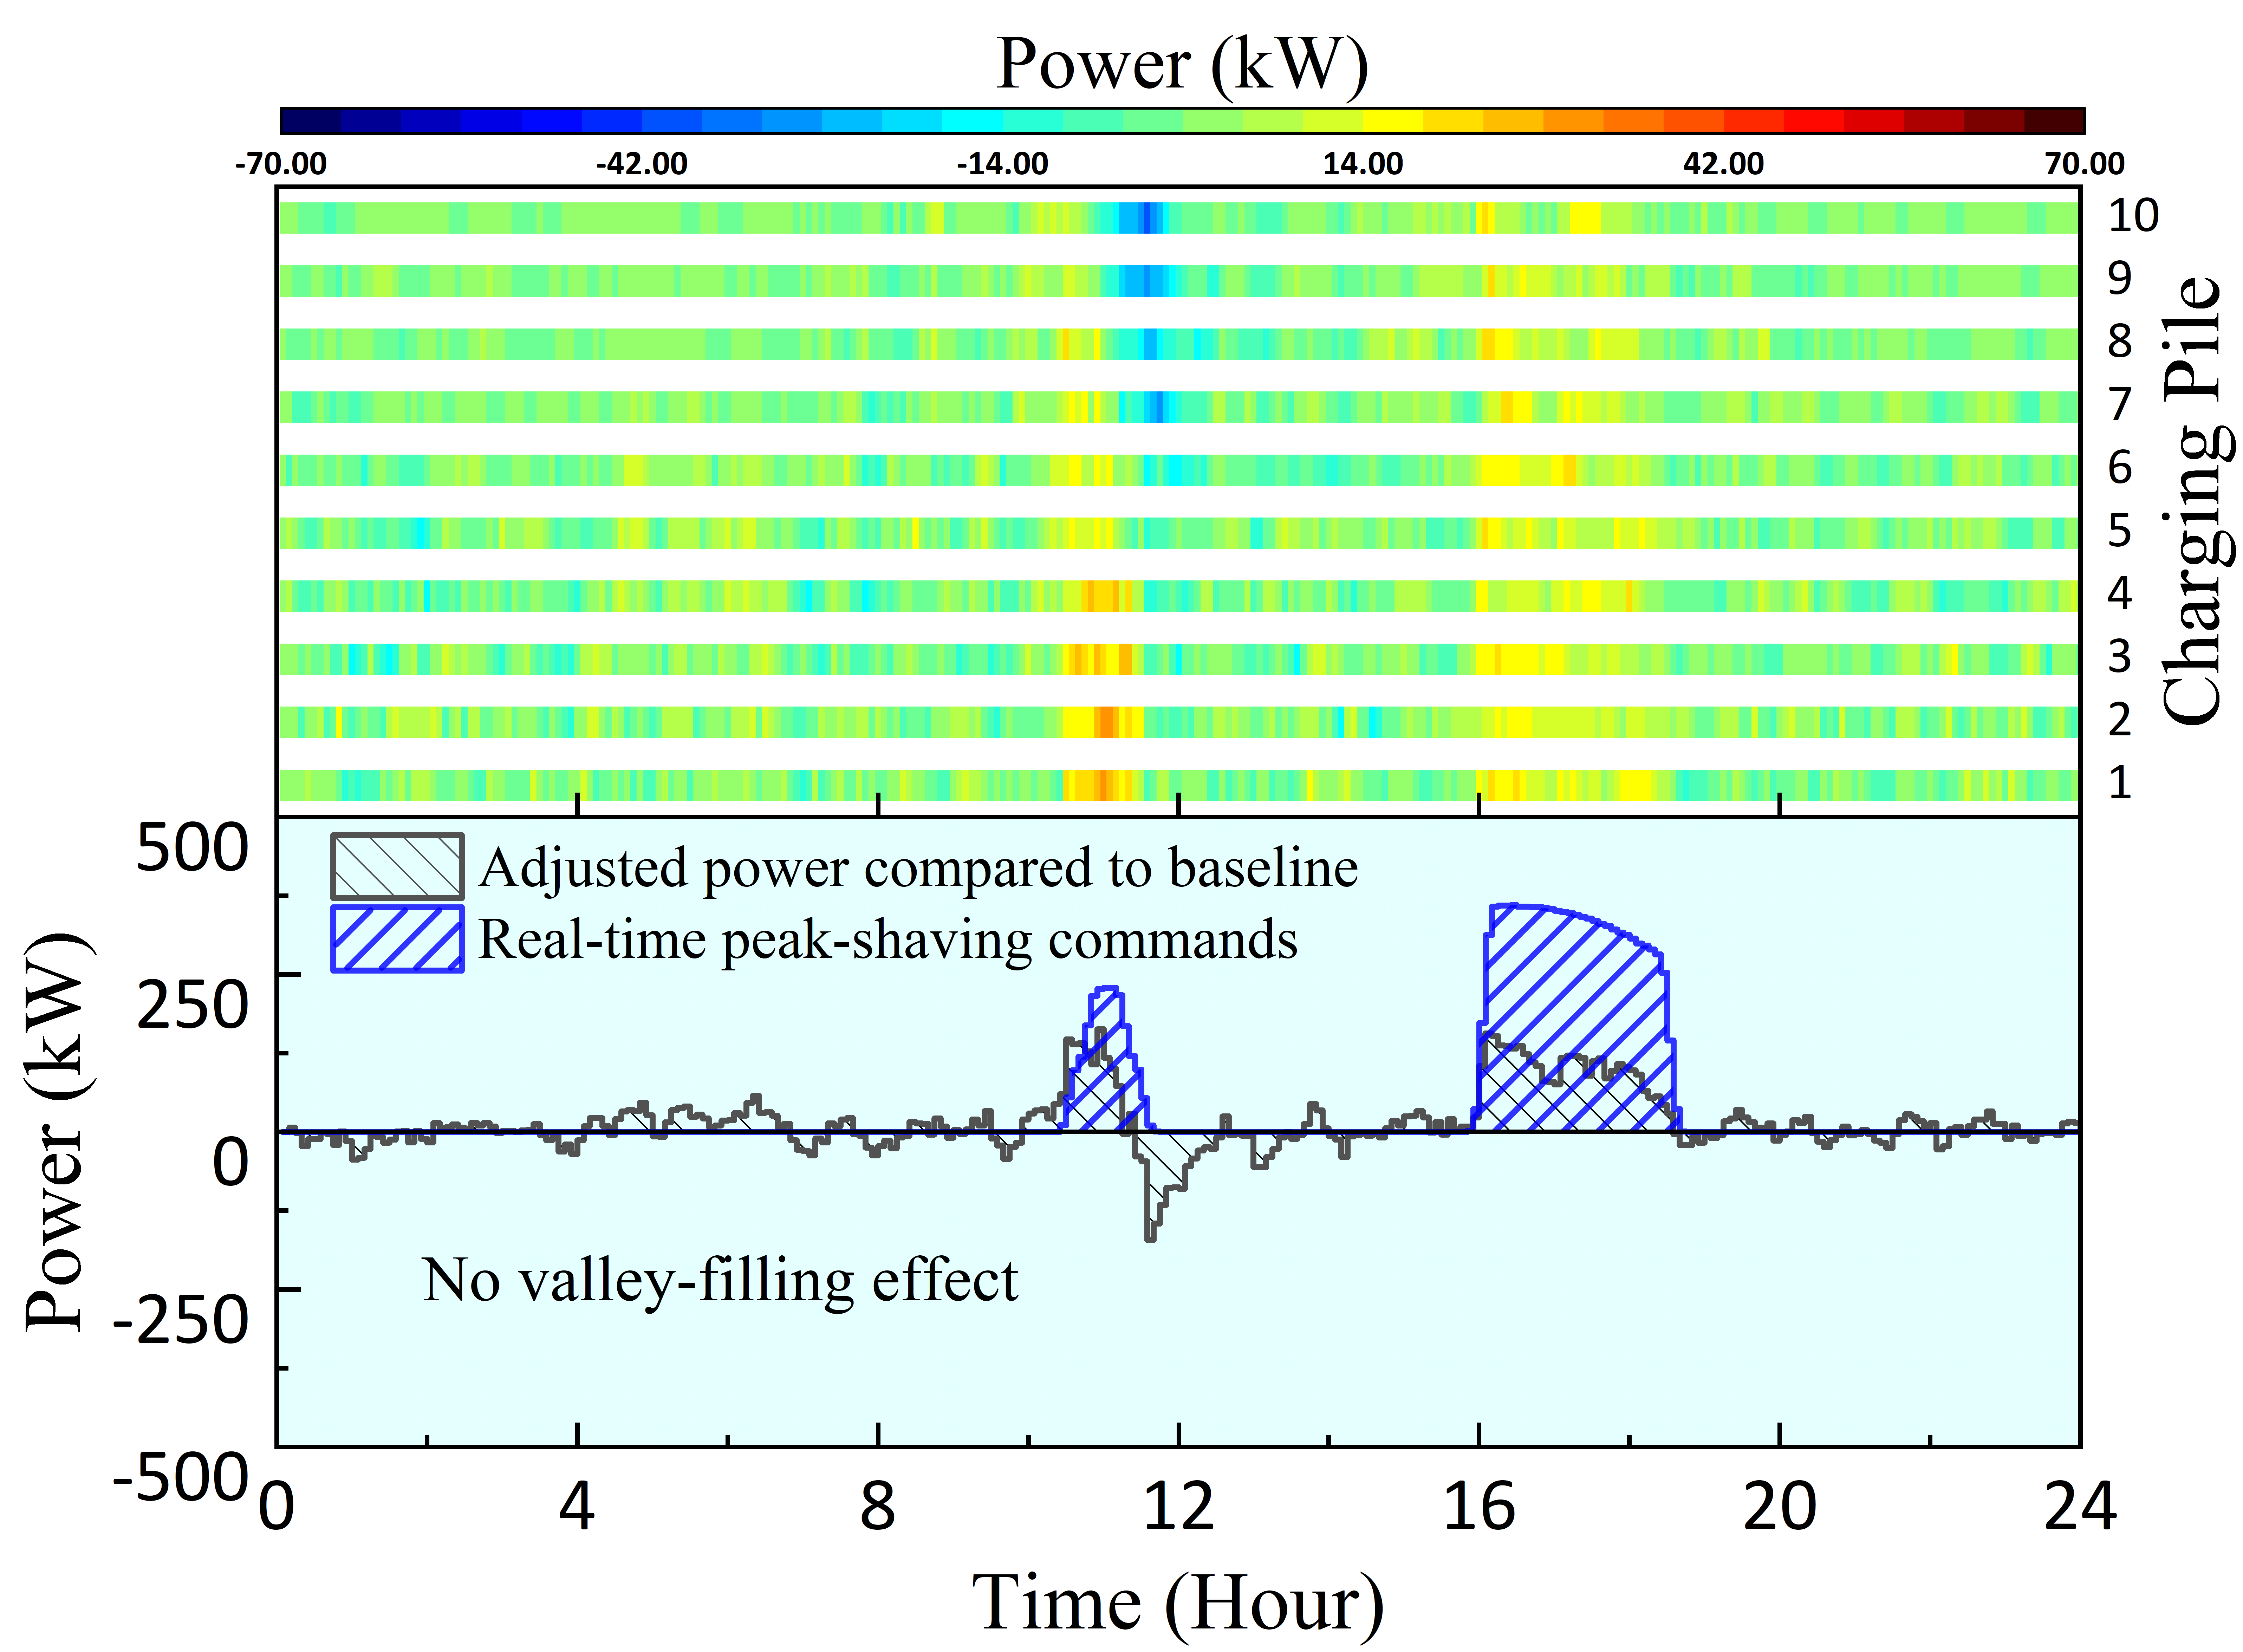
\includegraphics[width=0.49\linewidth]{figures/sch3_heatmap}}
\par\end{centering}
\begin{centering}
\subfloat[\emph{Sch-\mbox{IV}.}]{\centering{}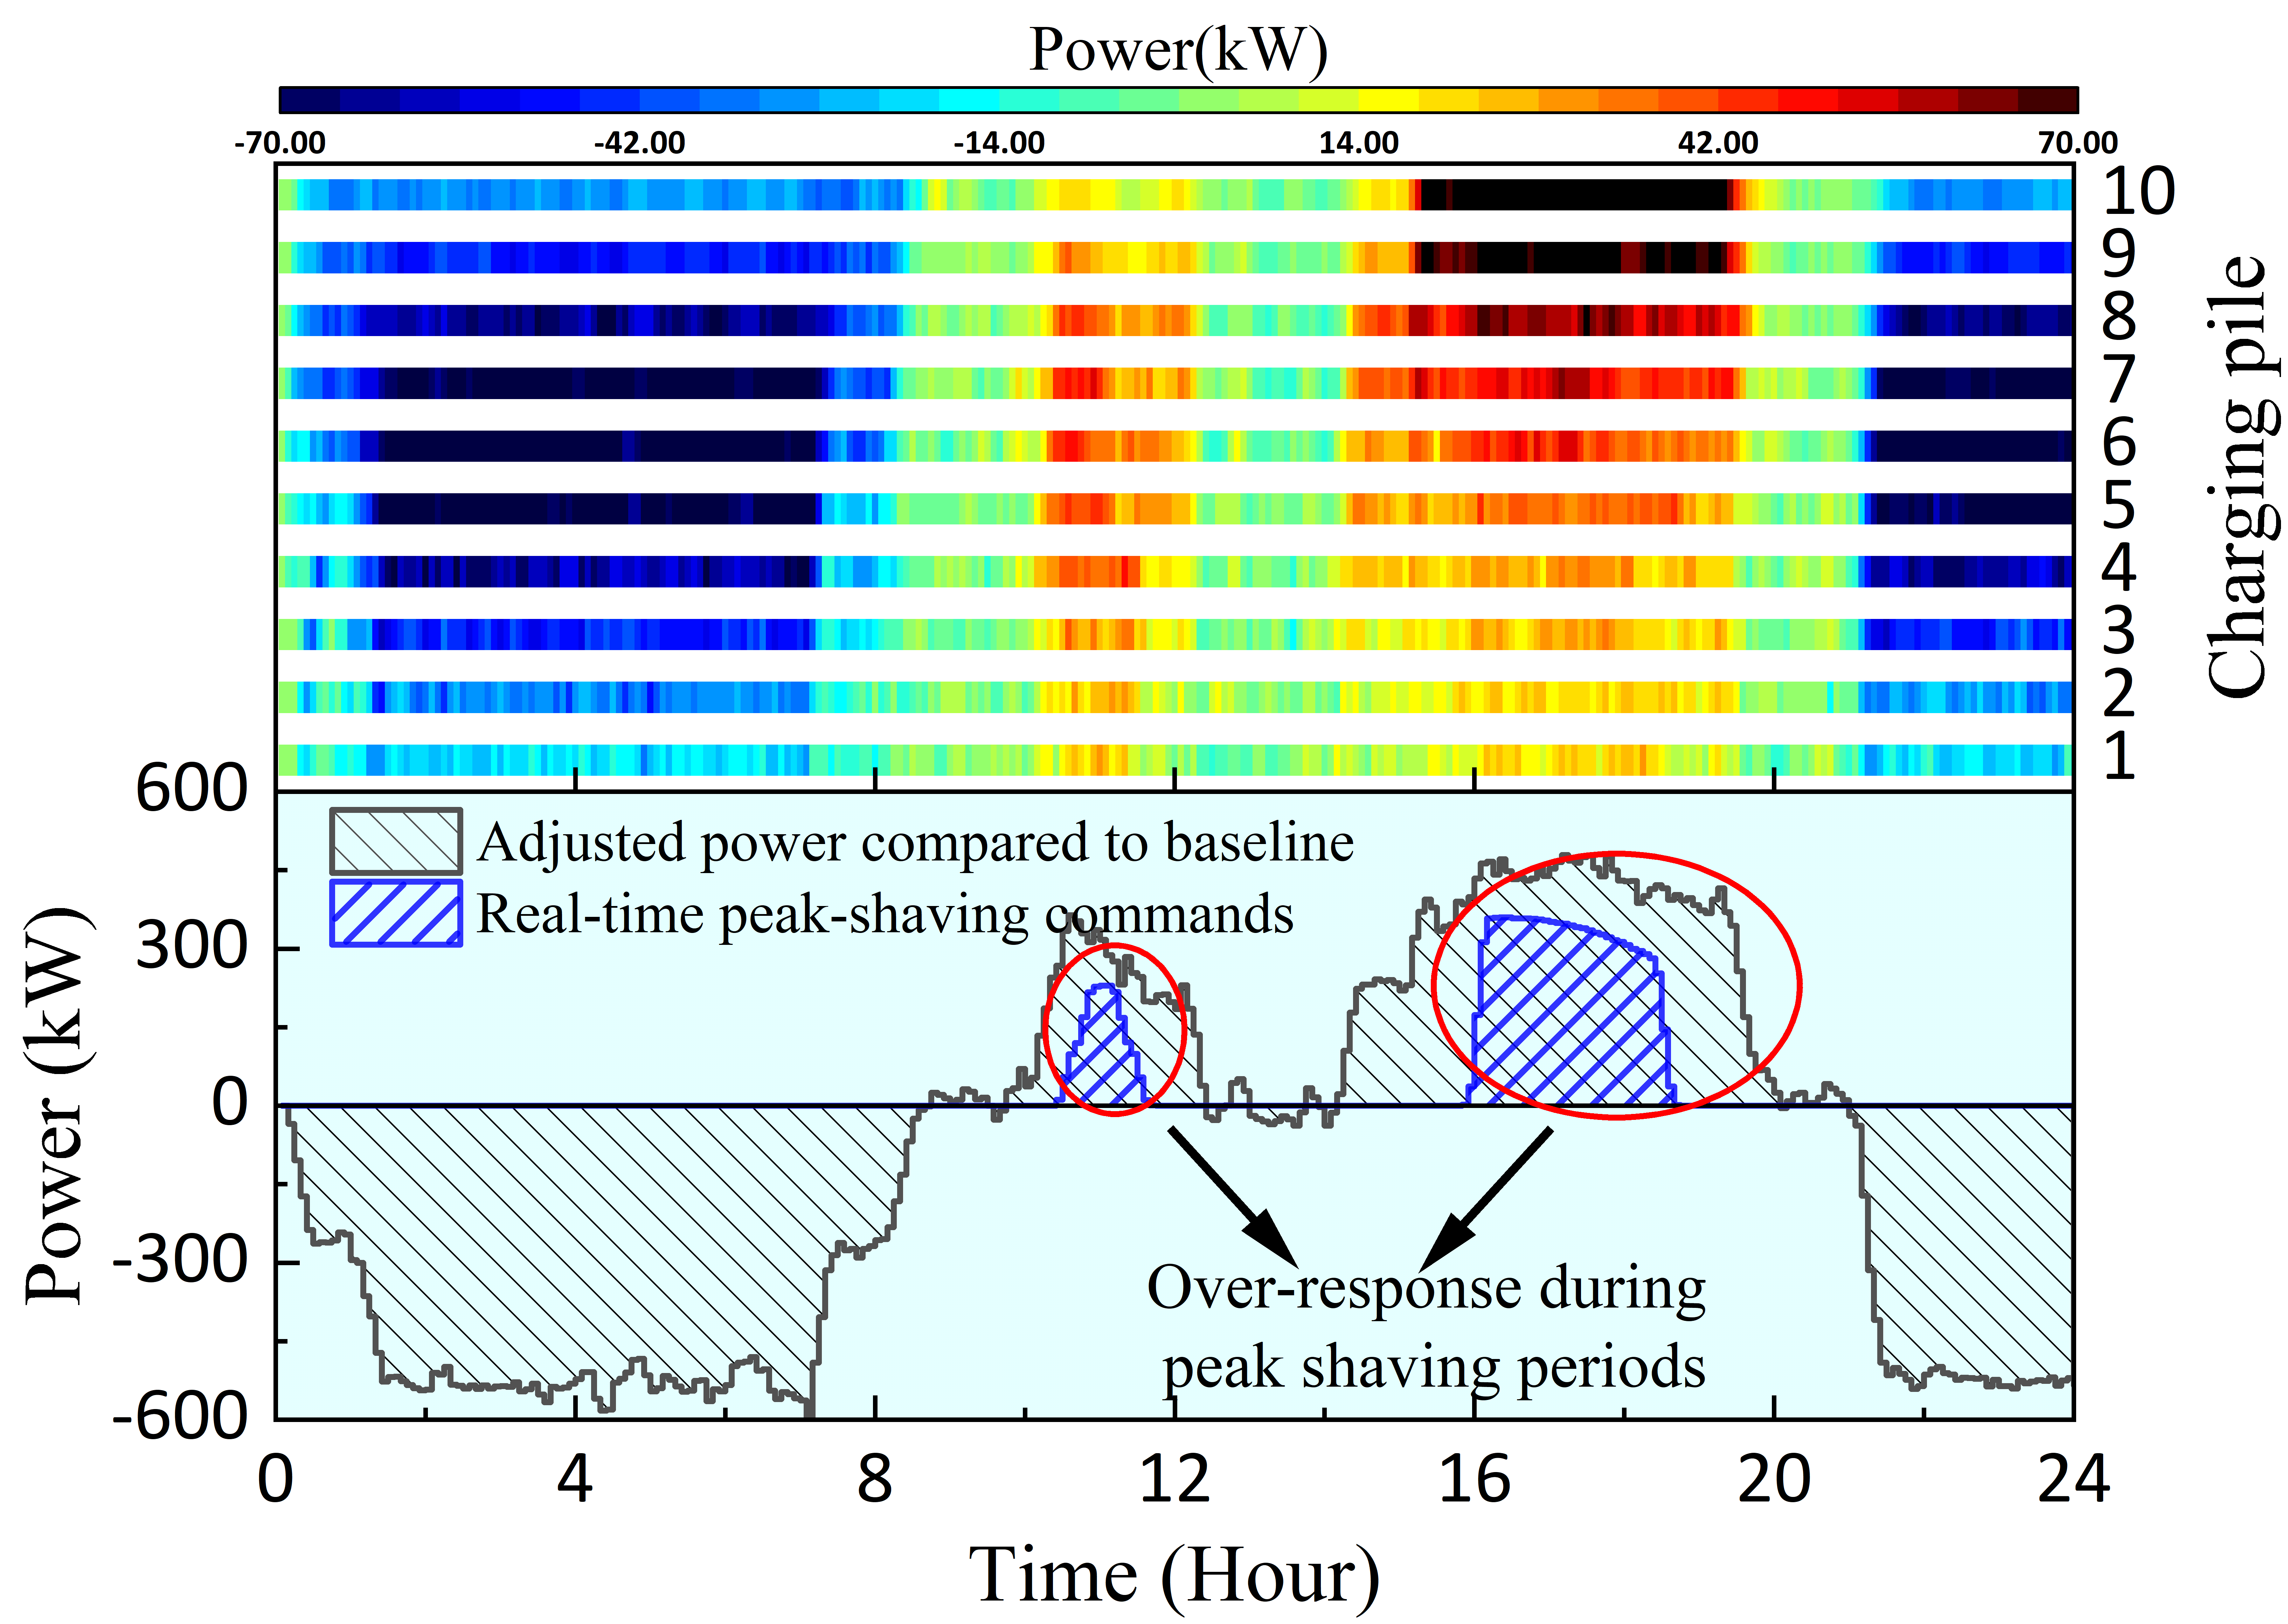
\includegraphics[width=0.49\linewidth]{figures/sch4_heatmap}}\subfloat[\emph{Sch-\mbox{V}.}]{\centering{}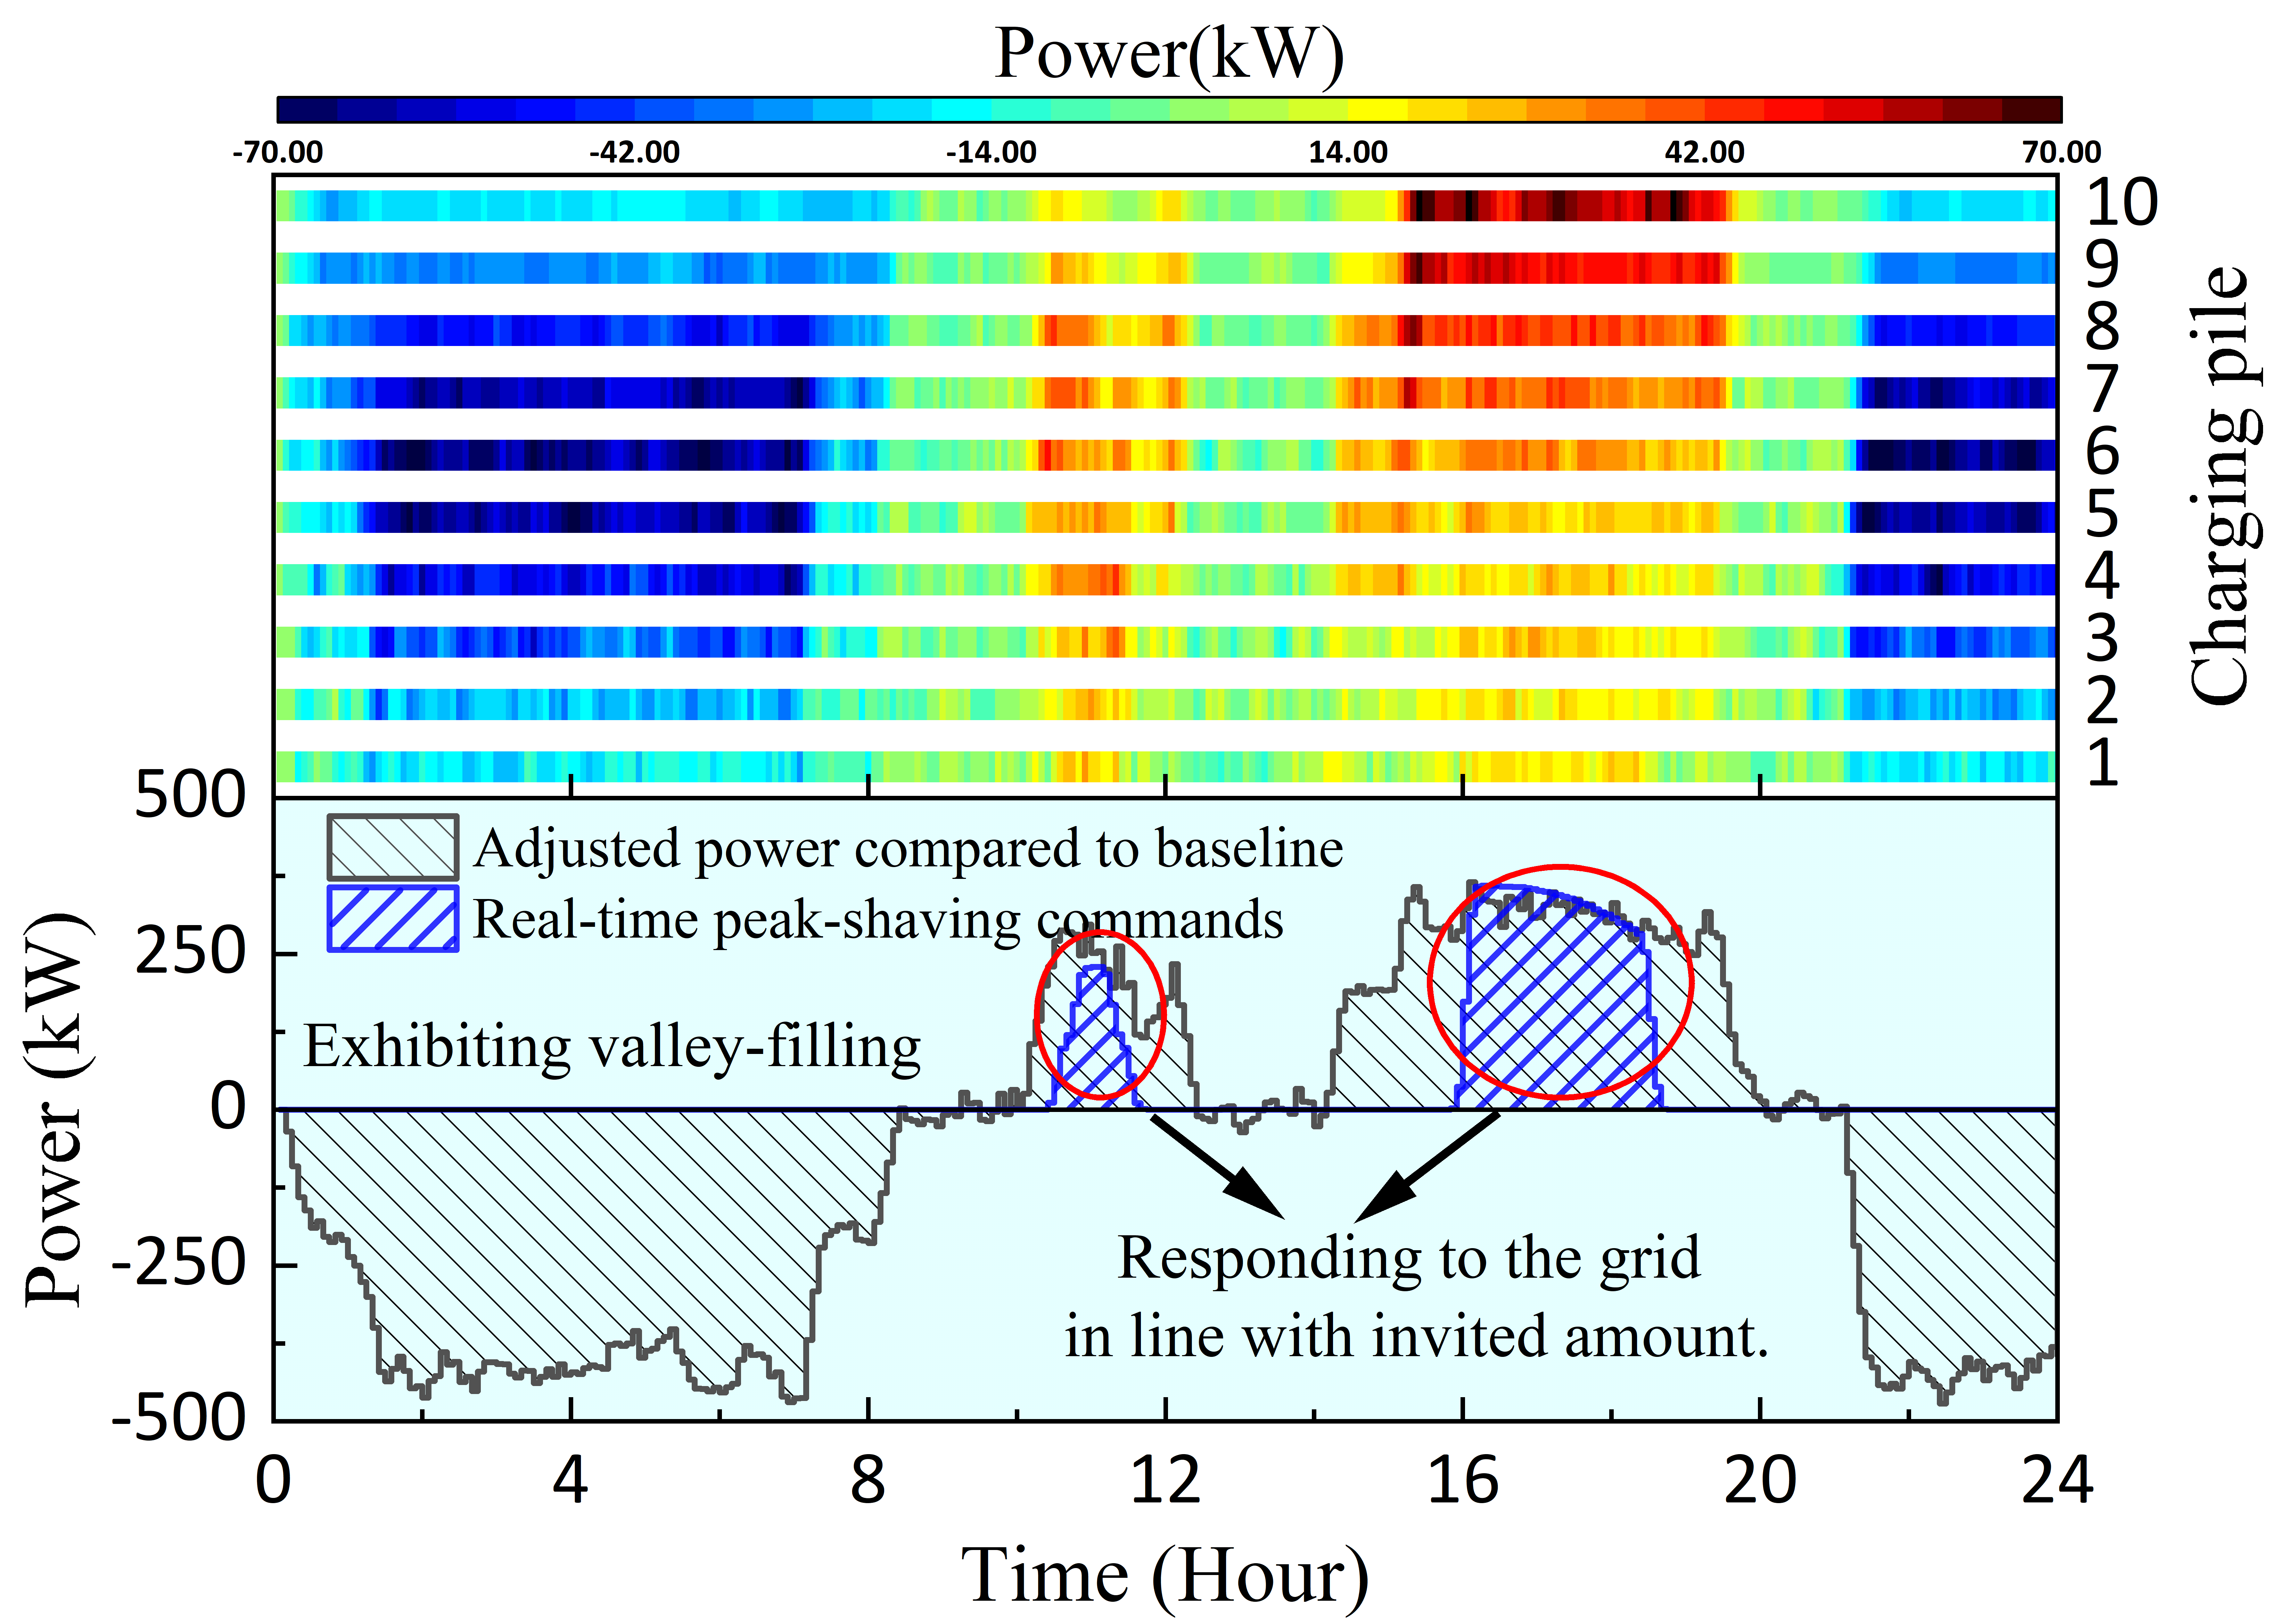
\includegraphics[width=0.49\linewidth]{figures/sch5_heatmap}}
\par\end{centering}
\caption{Charging Power Response in \emph{Sch-\mbox{II}, \mbox{III}, \mbox{IV} and \mbox{V}}.}
\label{fig:Charging-Power-Response}
\end{figure}

\begin{figure*}[htb]
\begin{centering}
\subfloat[\emph{Sch-I}]{\centering{}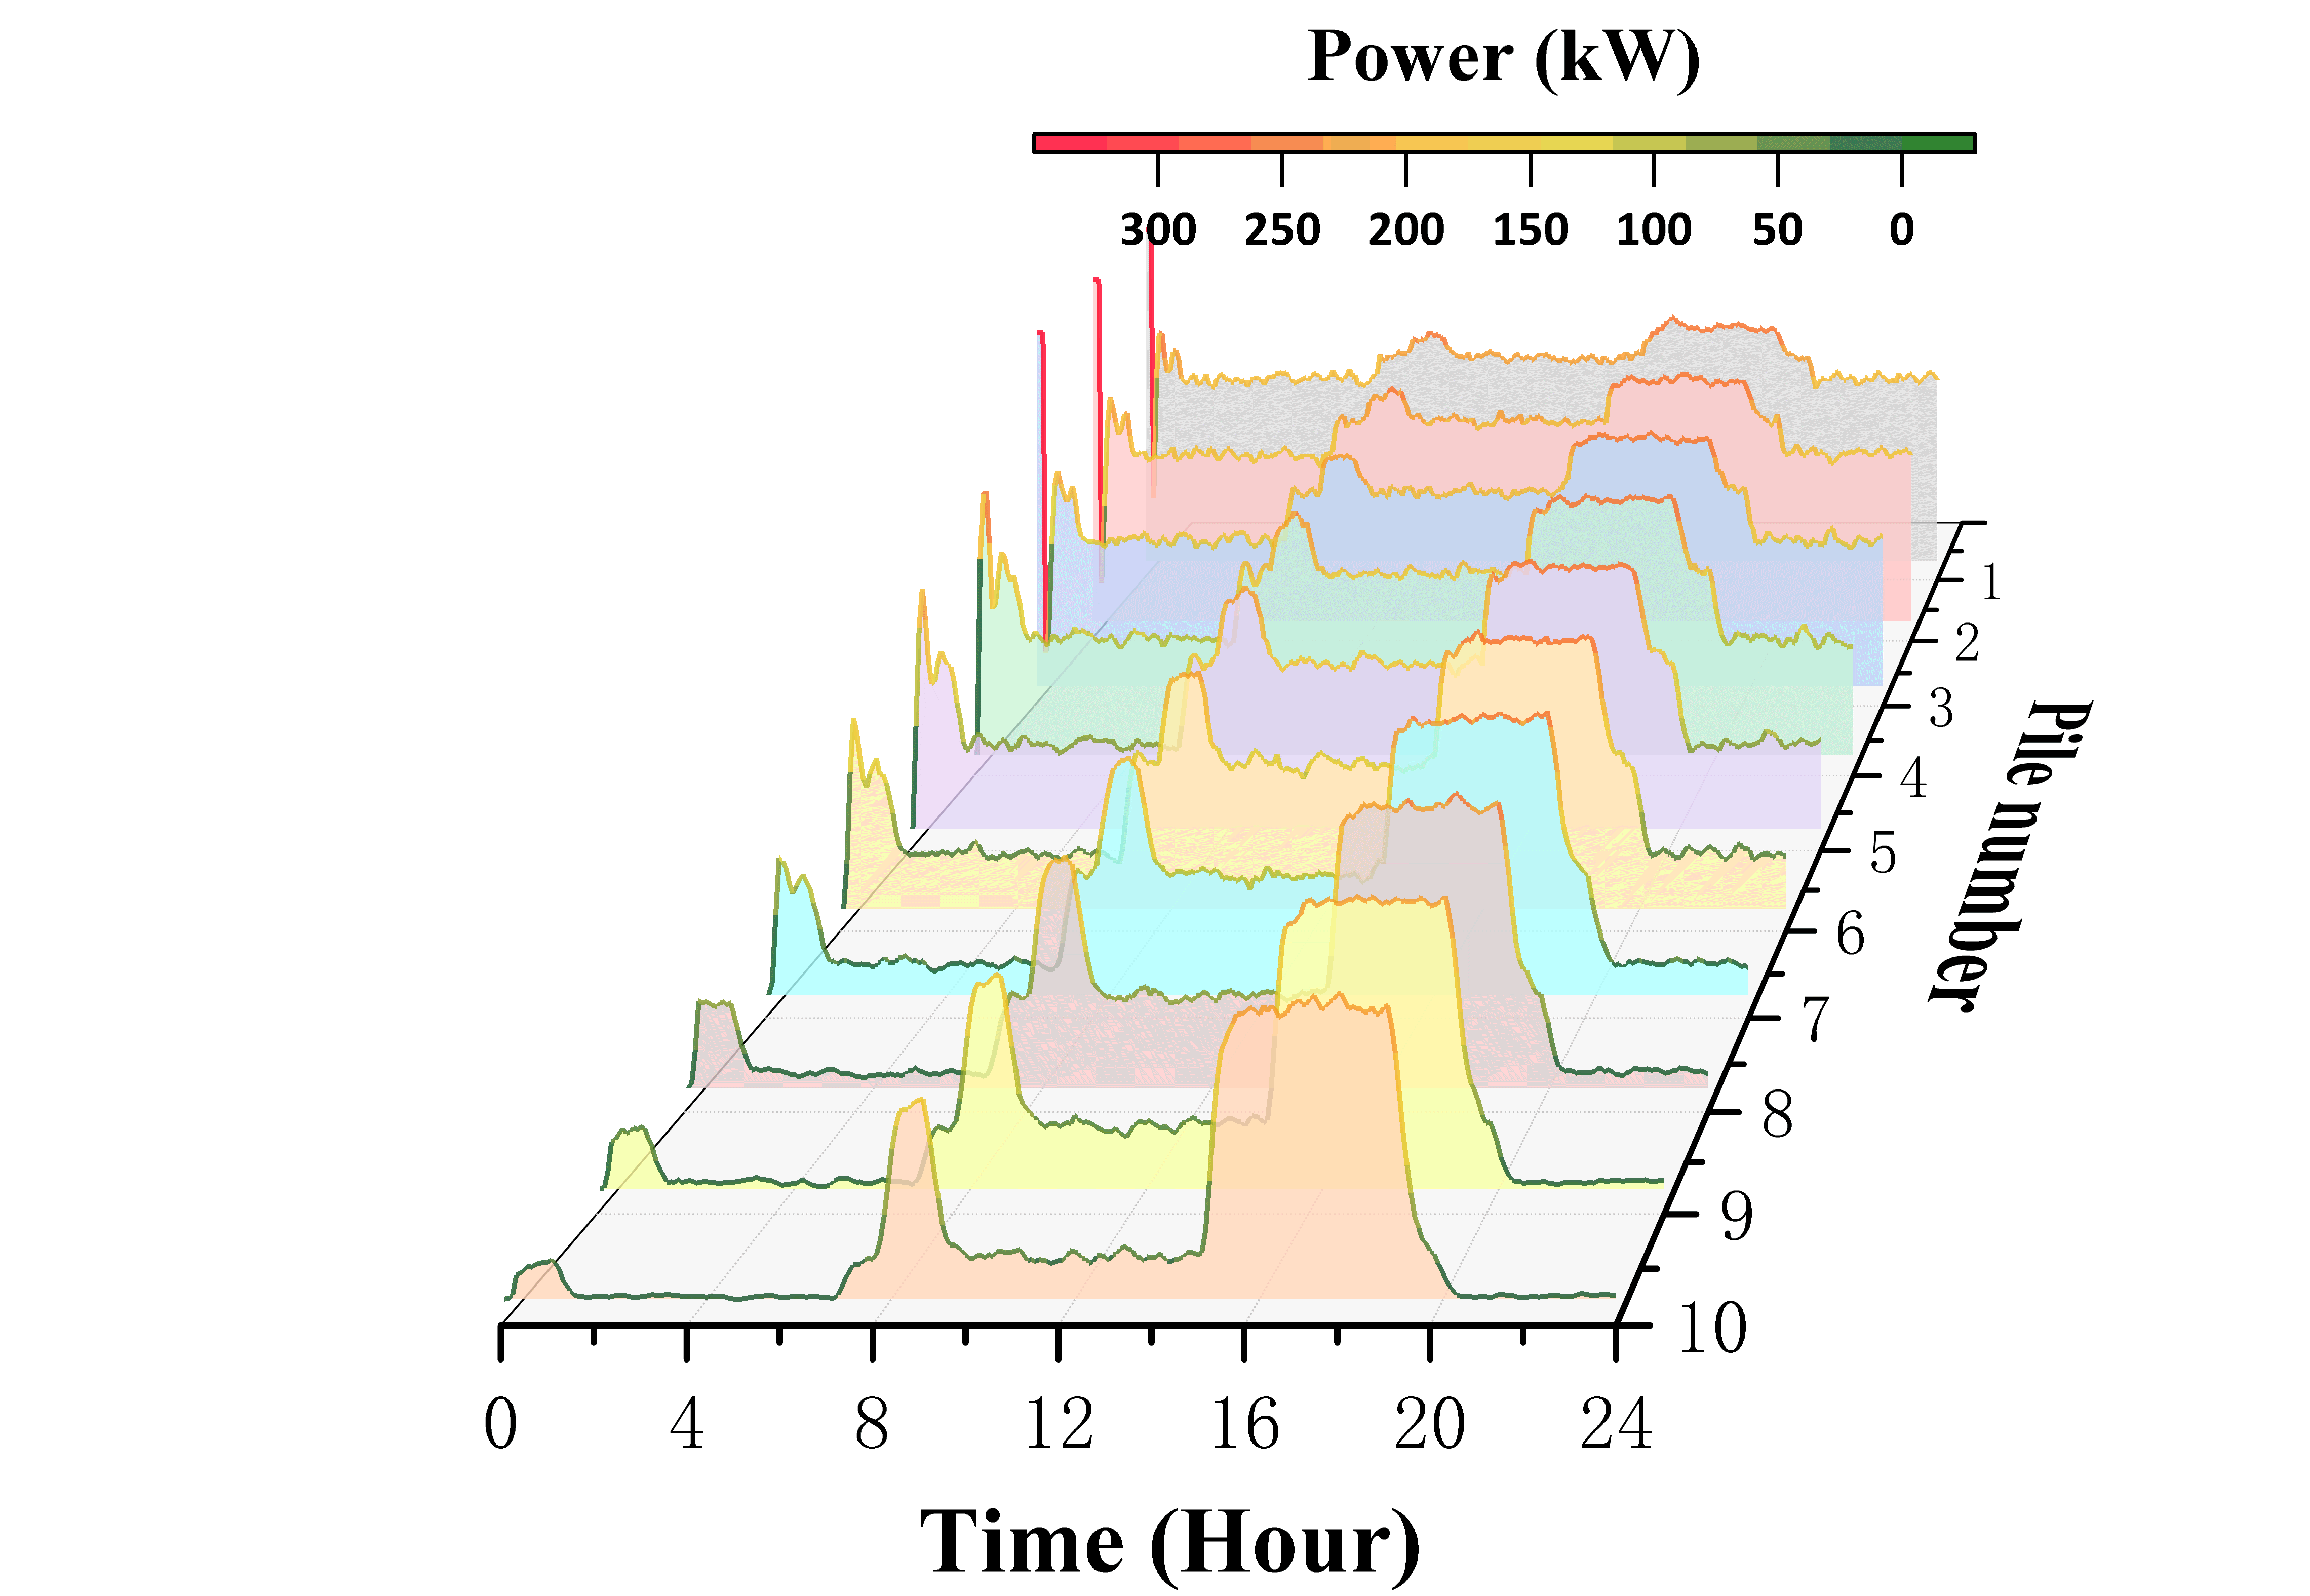
\includegraphics[width=0.33\linewidth,height=0.15\paperheight]{figures/sch1_pile_powers}}\subfloat[\emph{Sch-\mbox{II}}]{\centering{}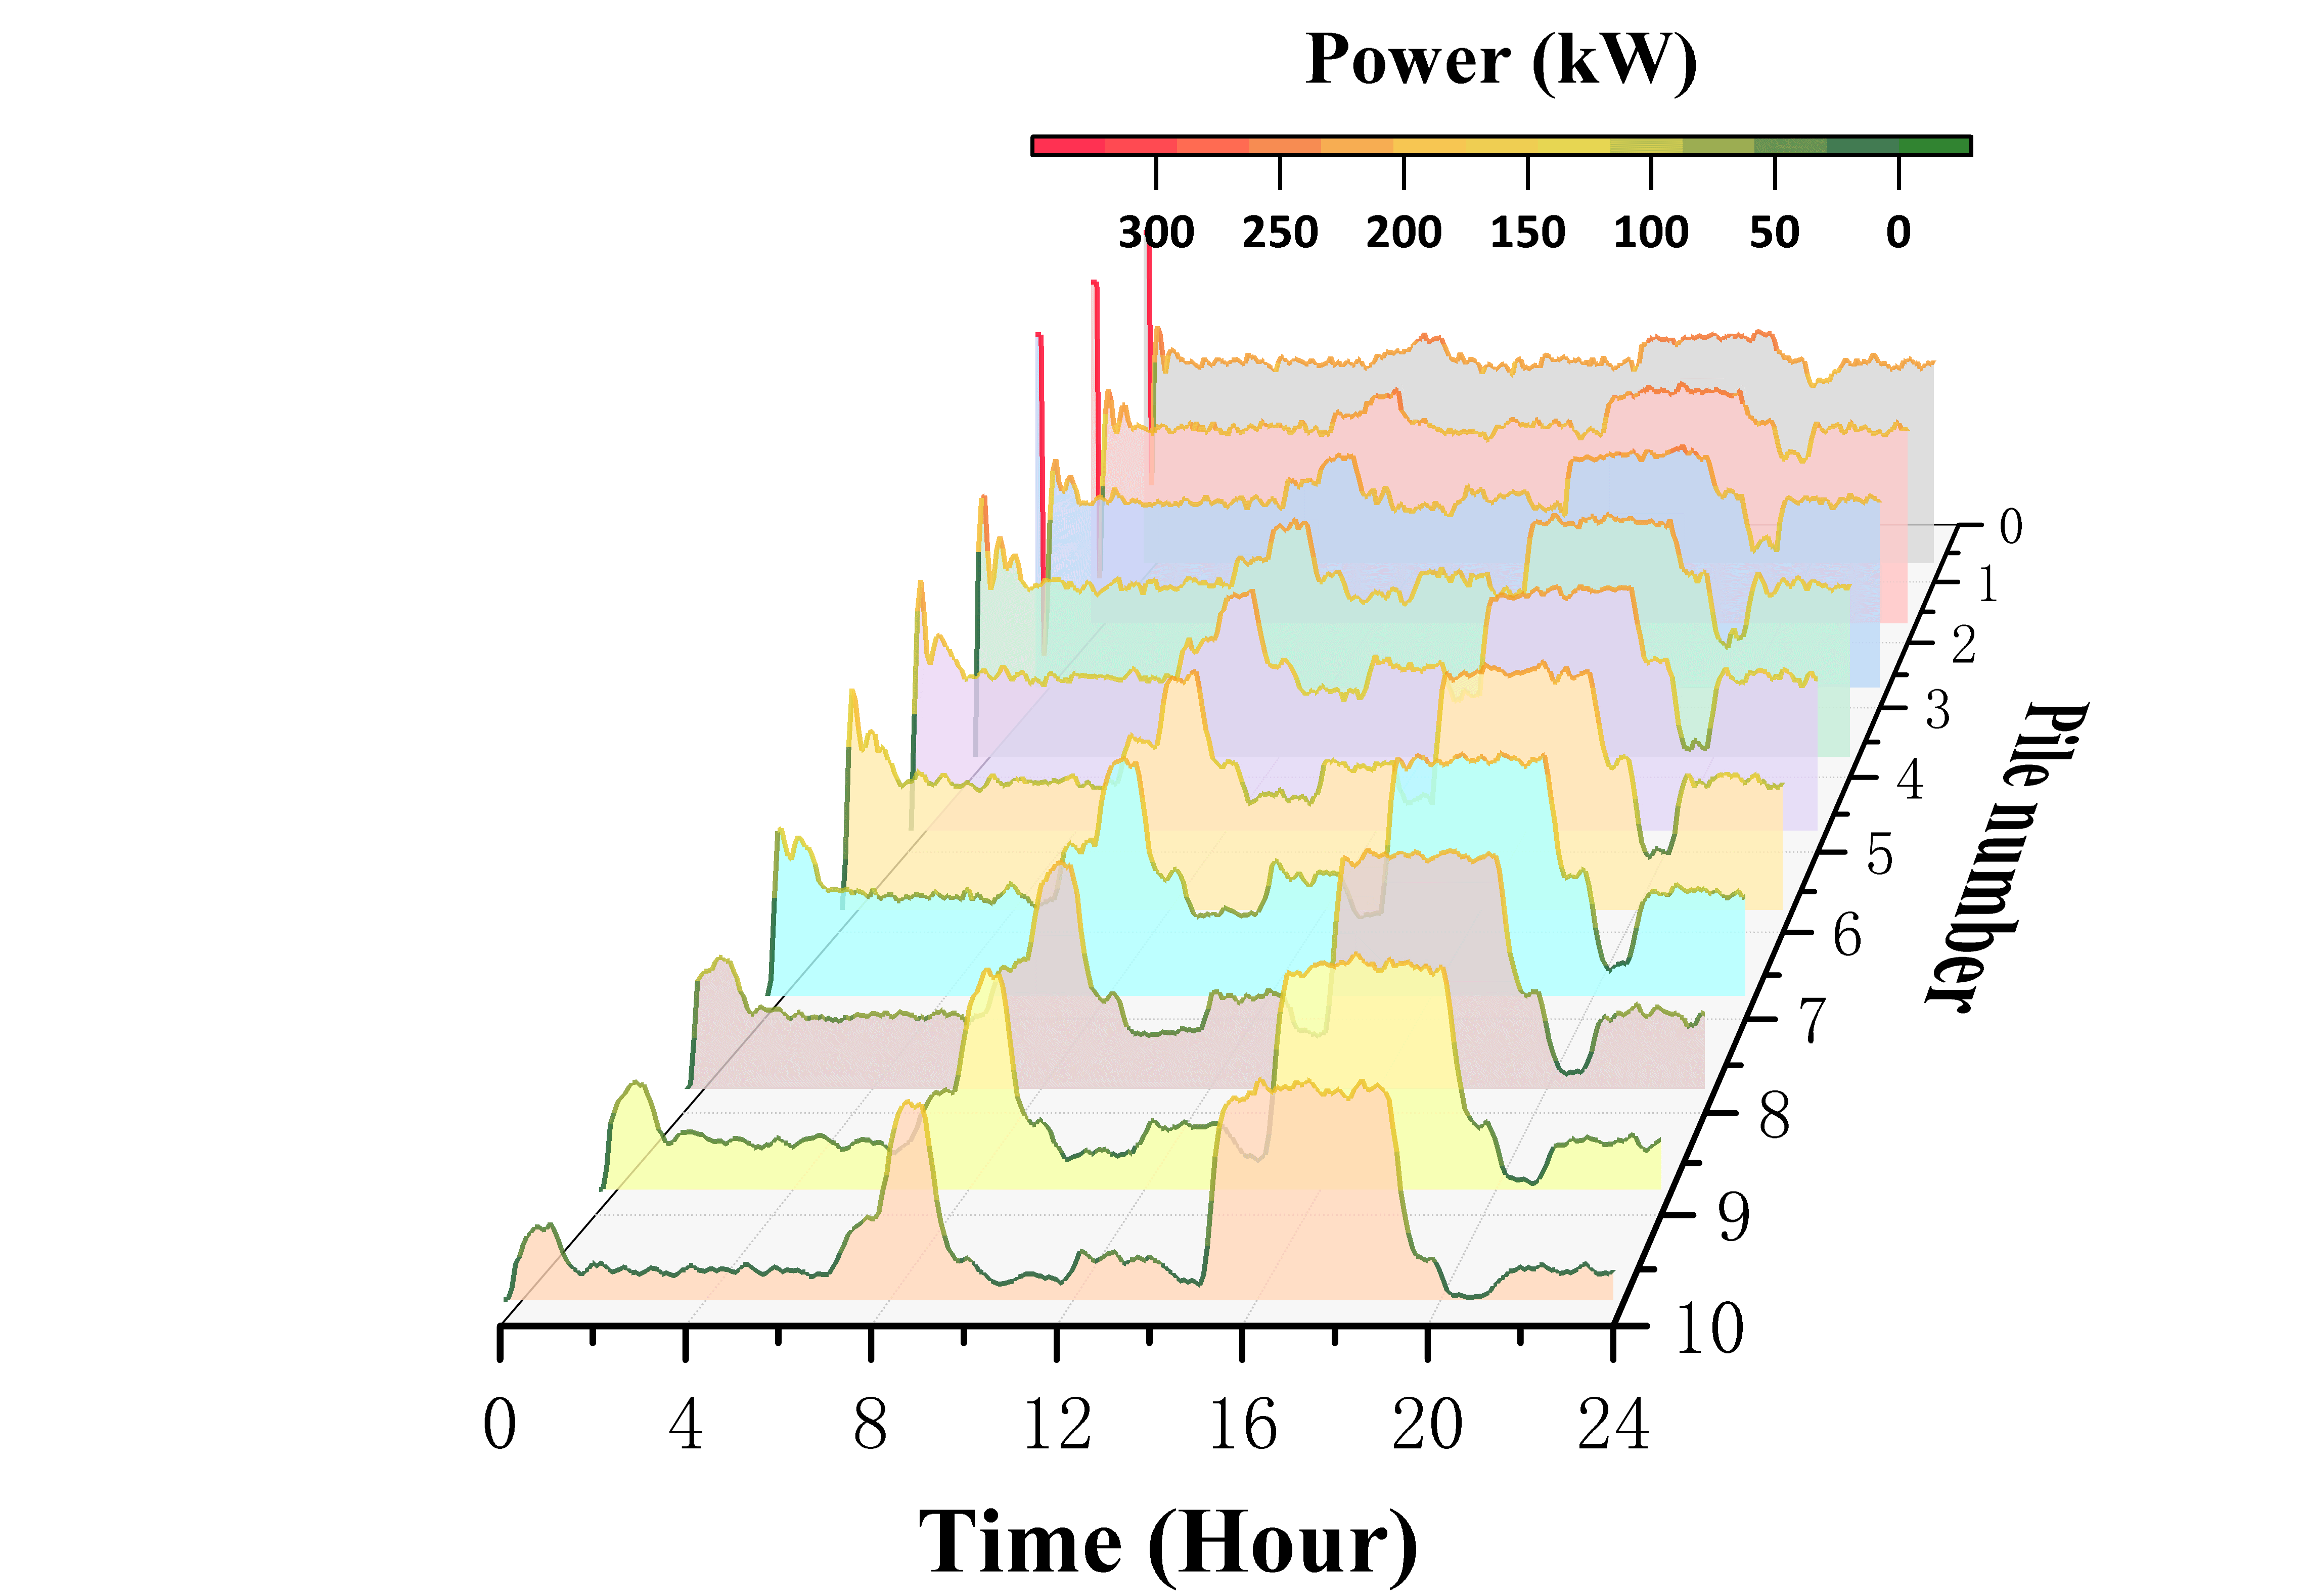
\includegraphics[width=0.33\linewidth,height=0.15\paperheight]{figures/sch2_pile_powers}}\subfloat[\emph{Sch-\mbox{III}}]{\centering{}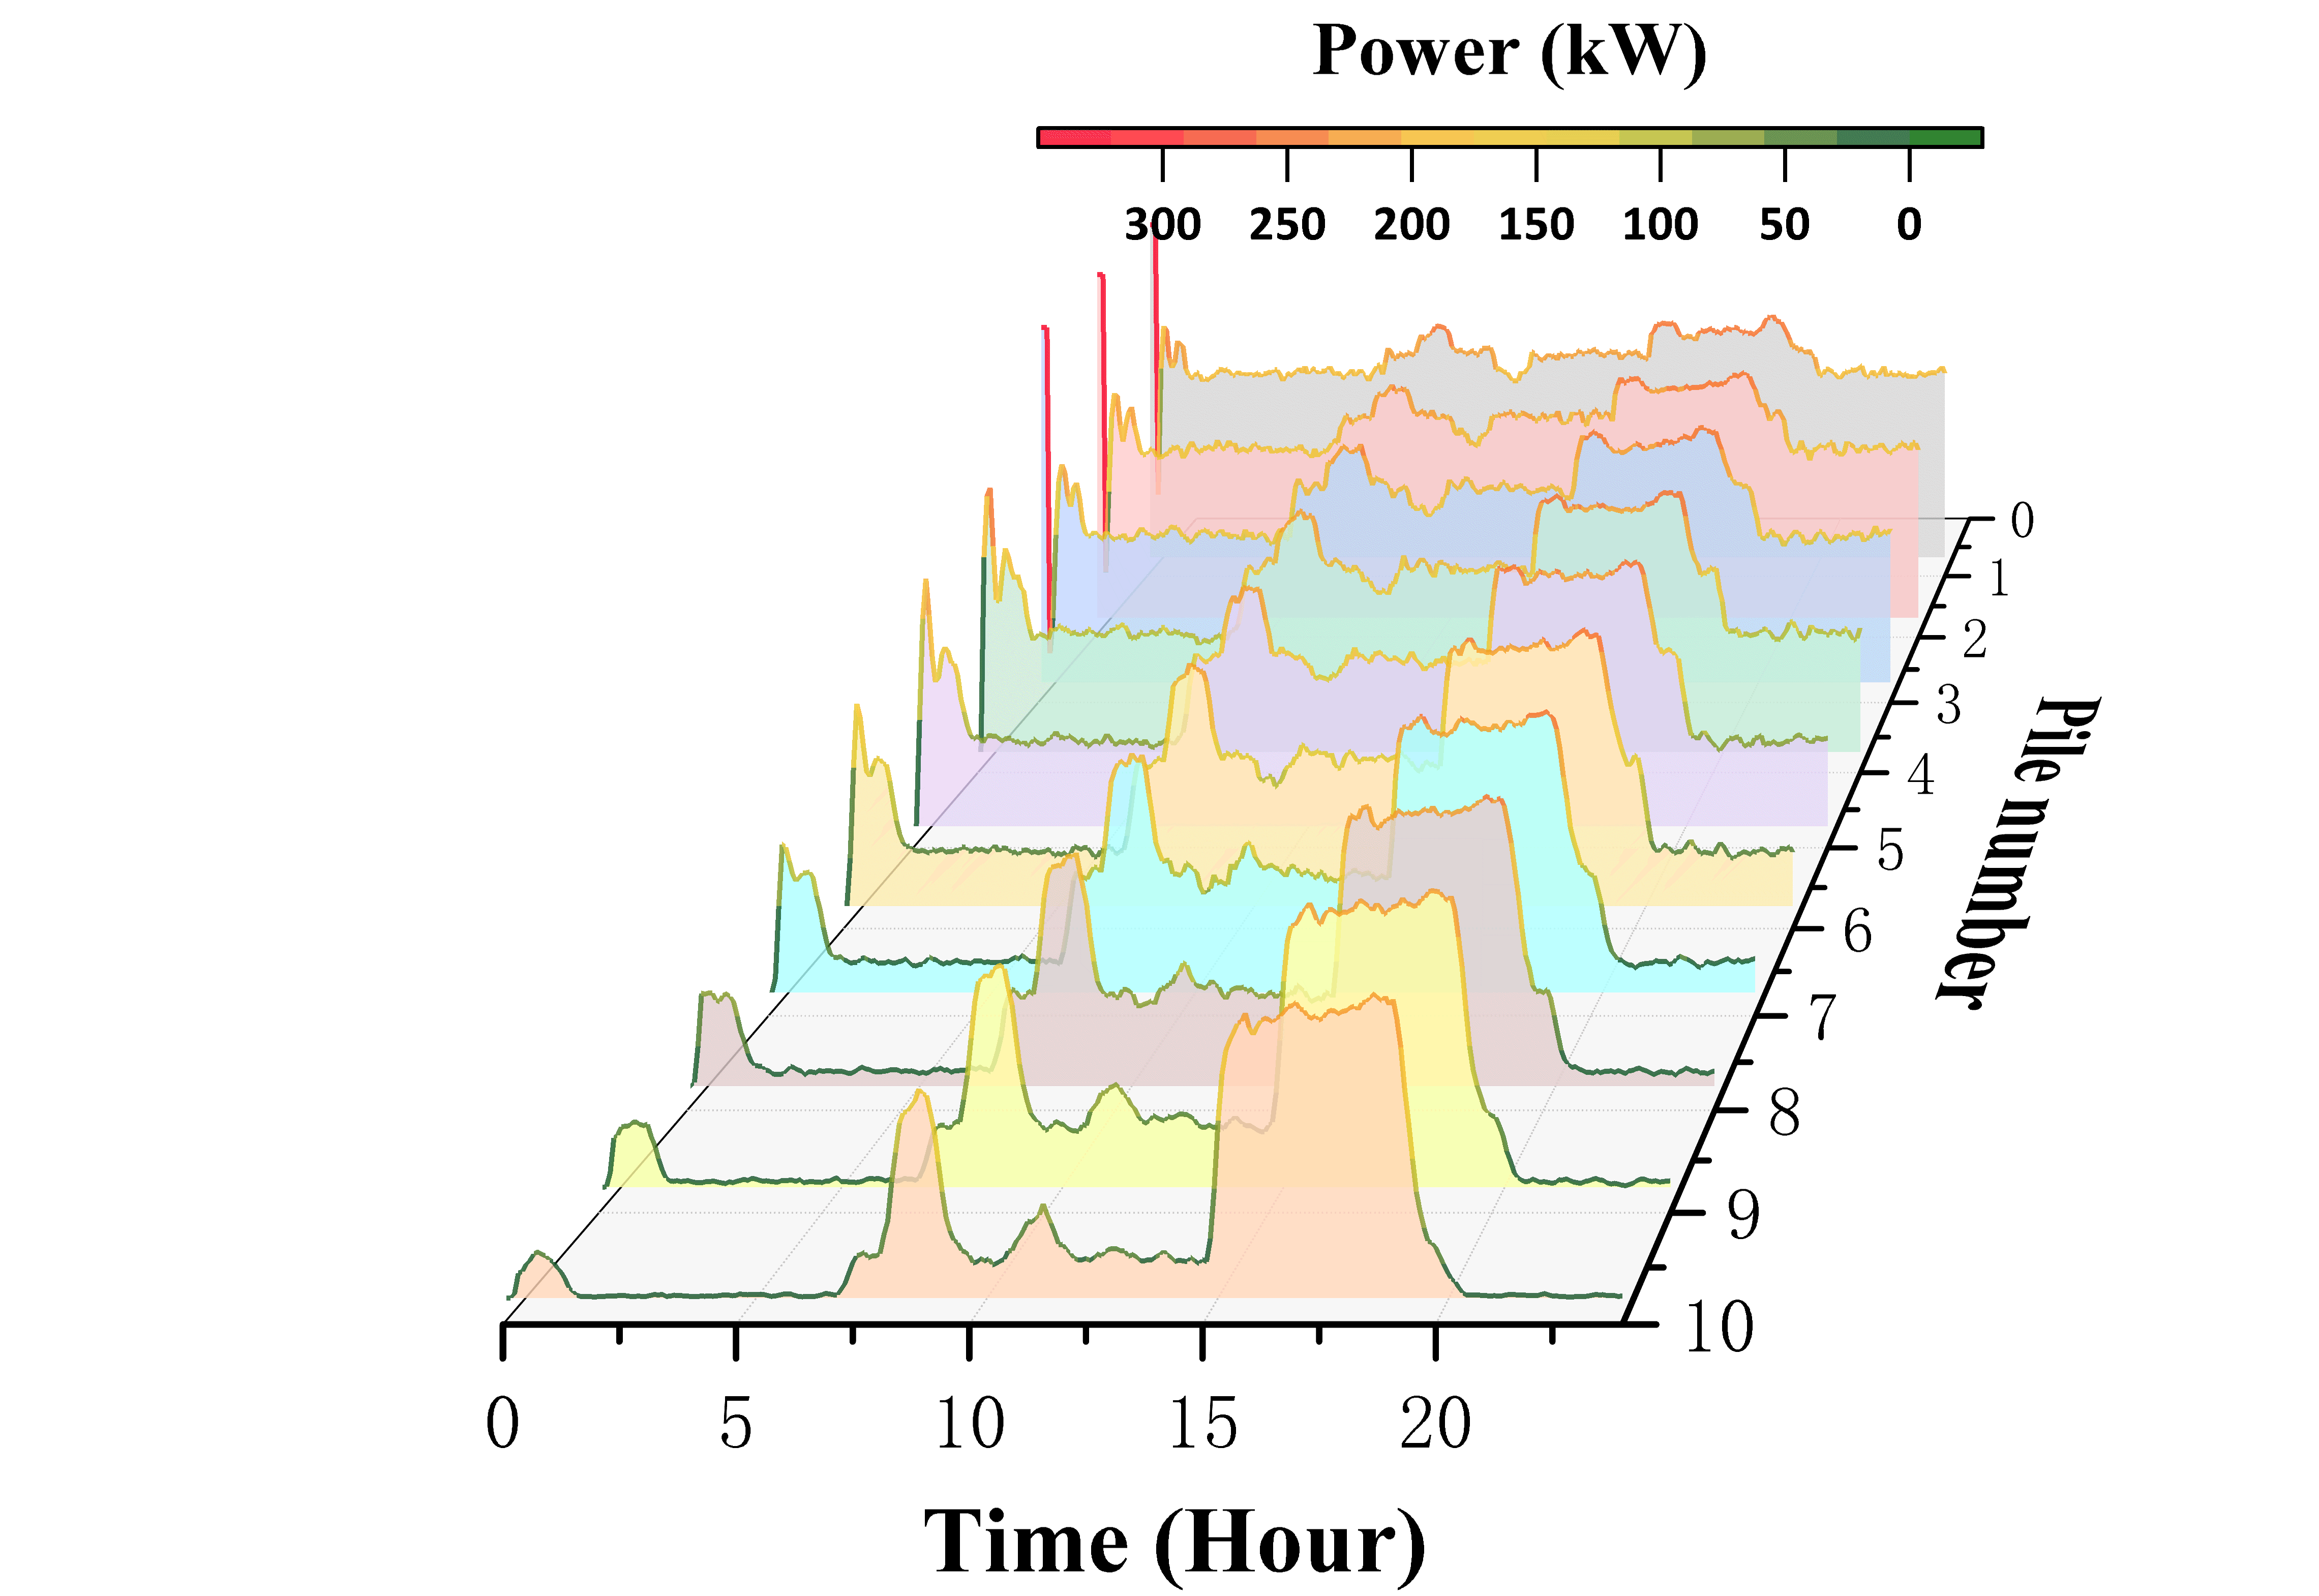
\includegraphics[width=0.33\linewidth,height=0.15\paperheight]{figures/sch3_pile_powers}}
\par\end{centering}
\begin{centering}
\subfloat[\emph{Sch-\mbox{IV}}]{\centering{}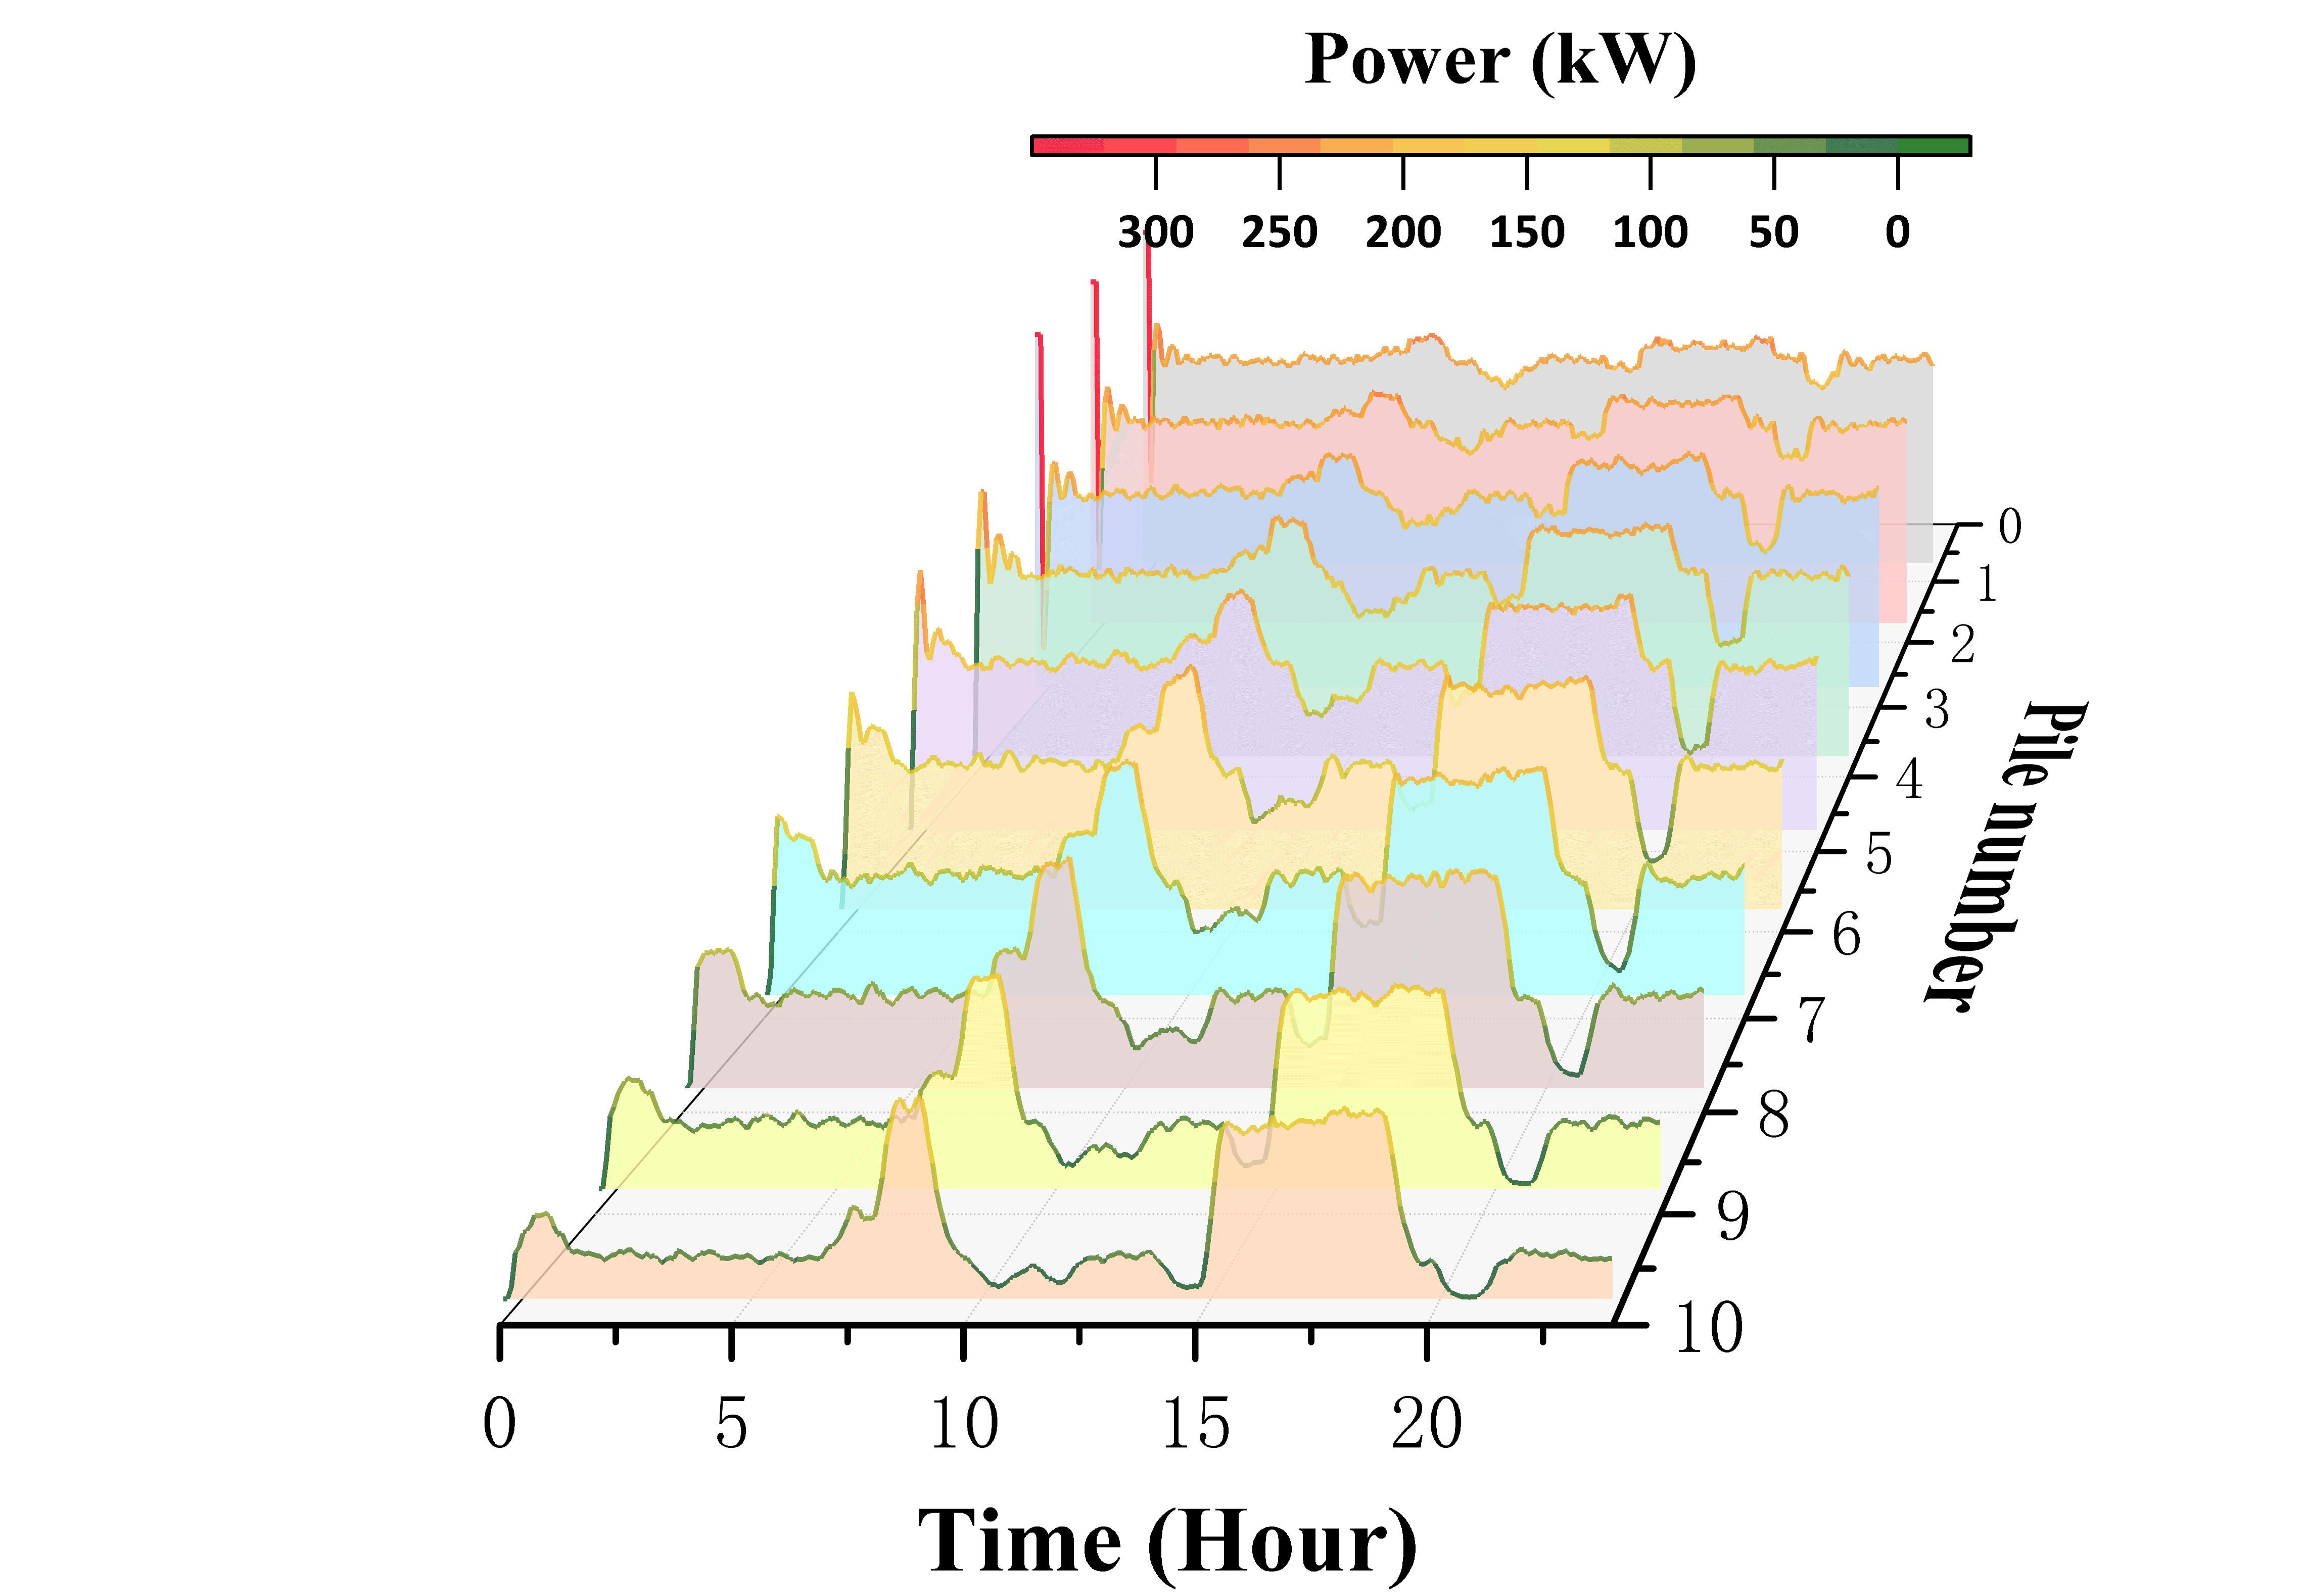
\includegraphics[width=0.33\linewidth,height=0.15\paperheight]{figures/sch4_pile_powers}}\subfloat[\emph{Sch-\mbox{V}}]{\centering{}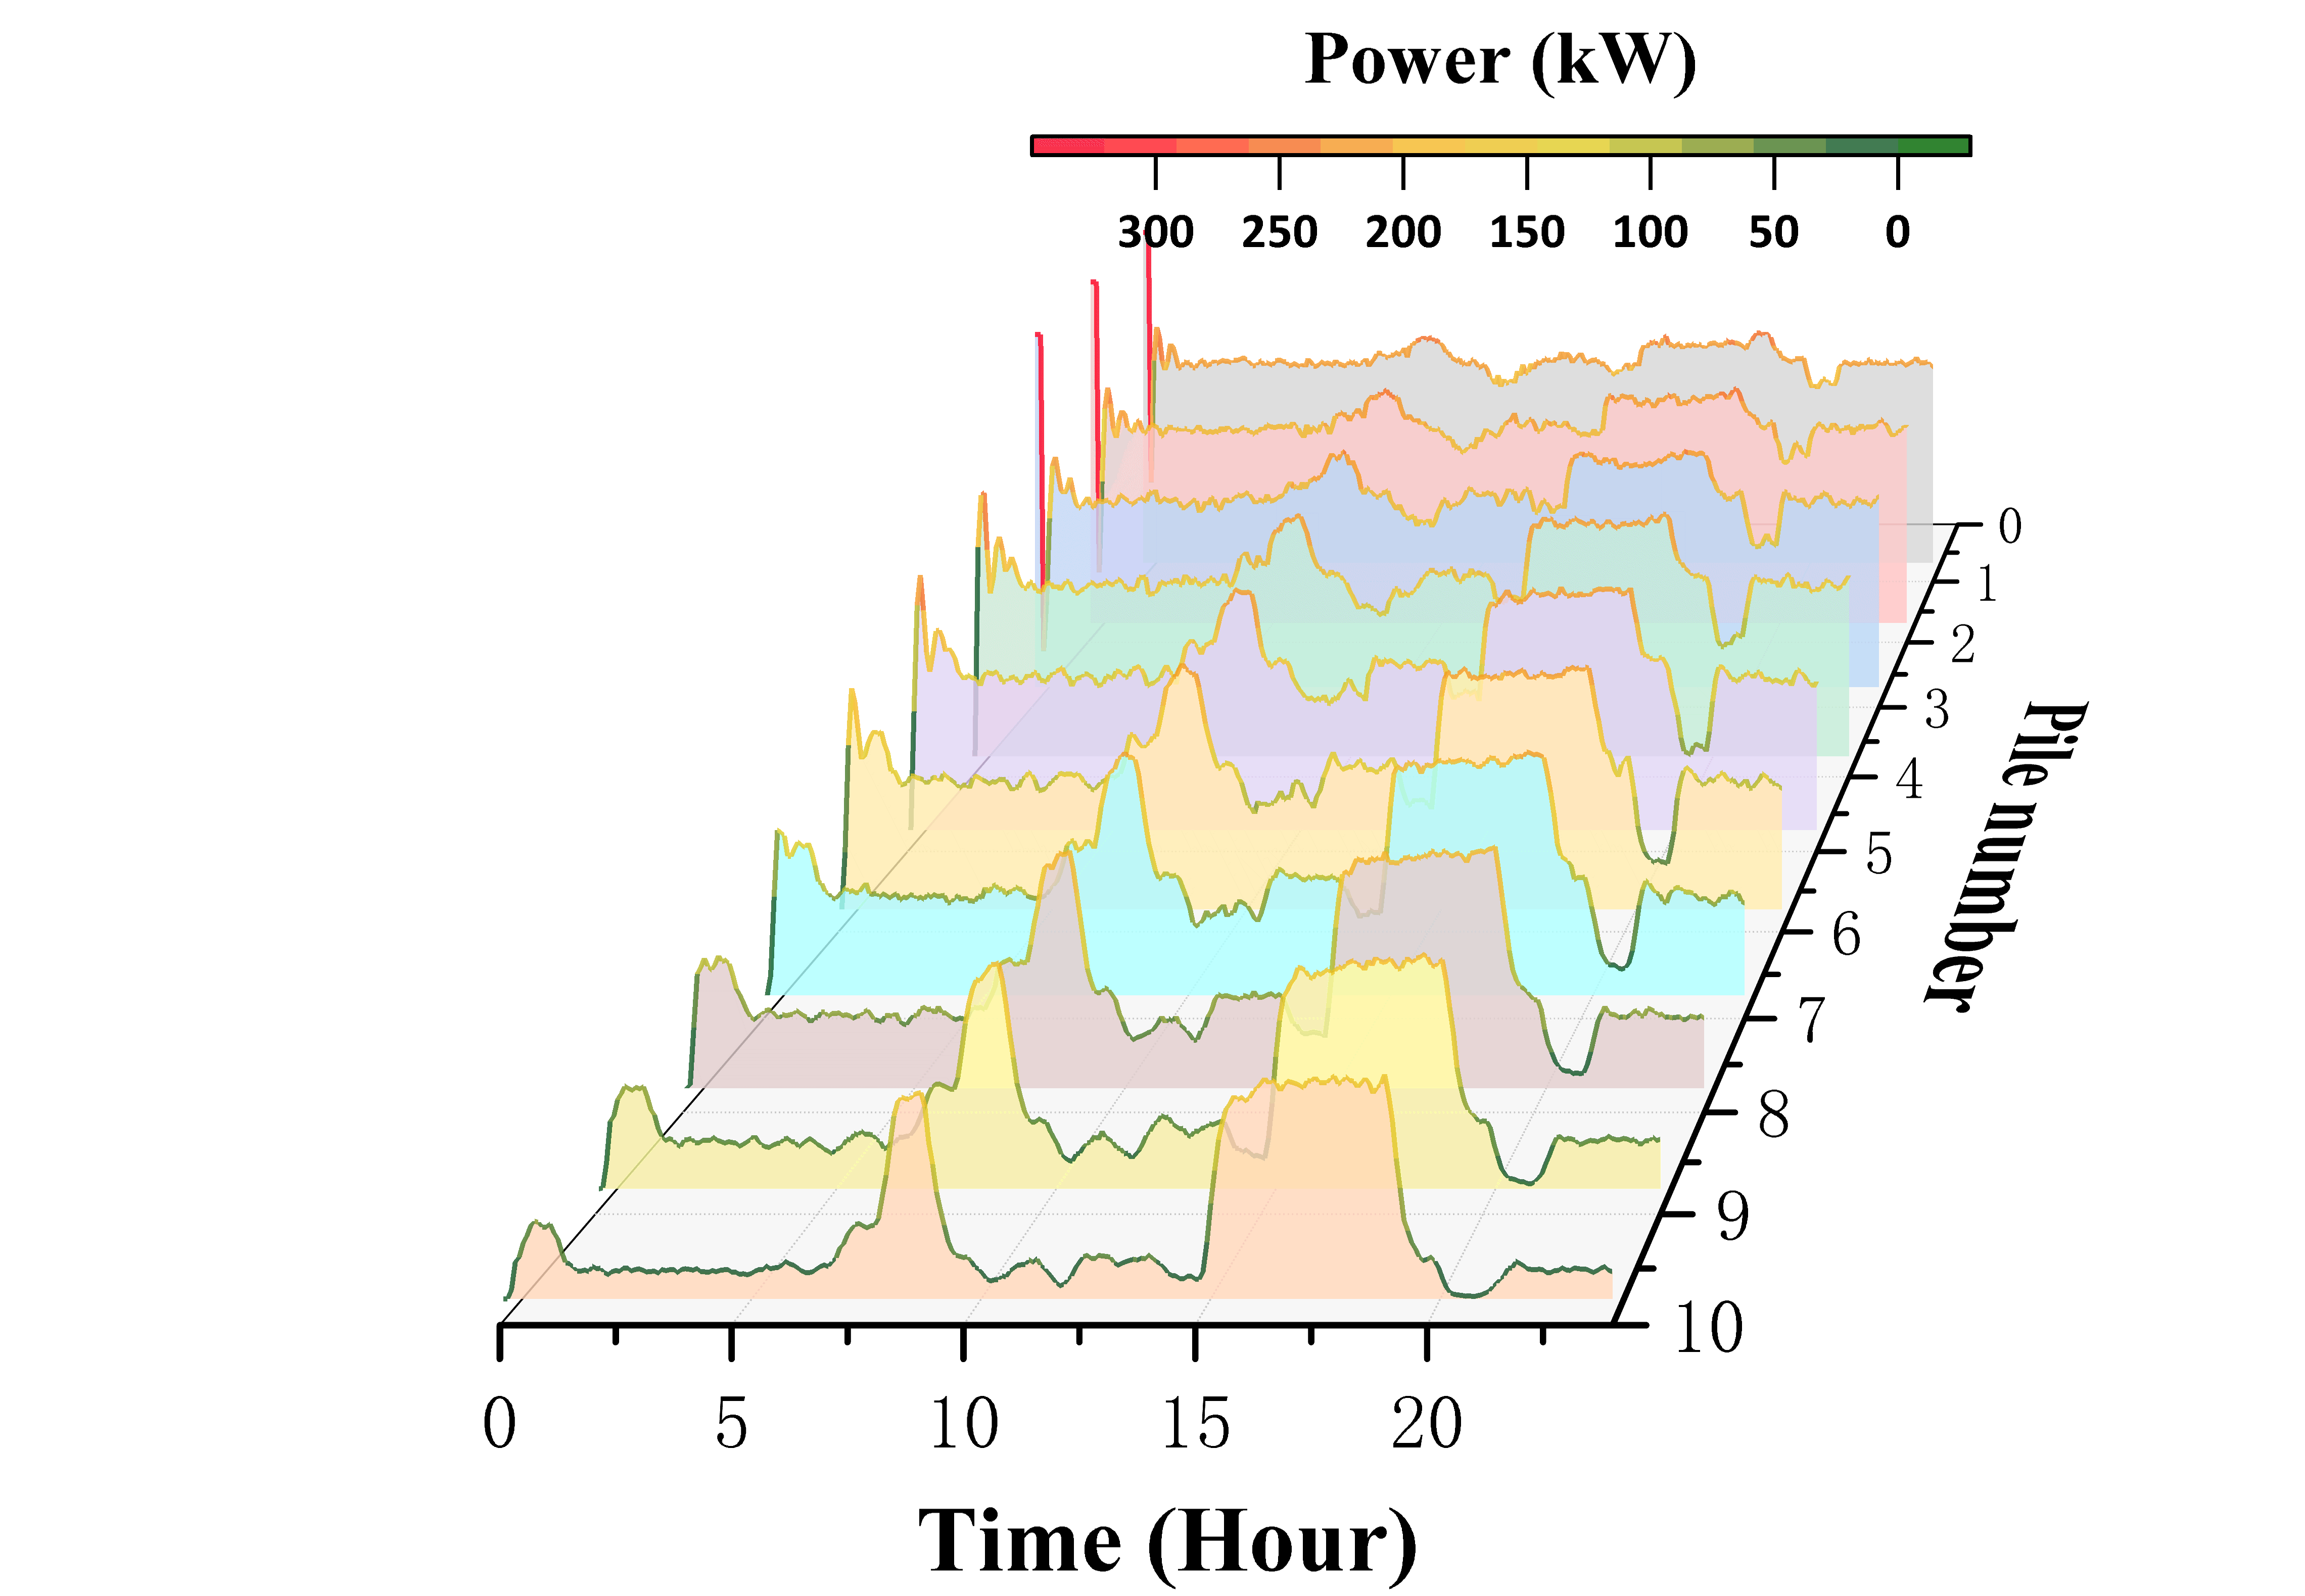
\includegraphics[width=0.33\linewidth,height=0.15\paperheight]{figures/sch5_pile_powers}}
\par\end{centering}
\caption{Charging Power Curves of 10 Charging Piles under five schemes}
\label{fig:Charging-Power-Curves3D}
\end{figure*}


\subsection{Analysis of Collaborative Optimization Strategy}

To assess the dual-center framework and collaborative optimization introduced in this paper, we conducted five experimental schemes within the same environmental simulation.  \emph{Sch-I}, the baseline, represents the standard station operation with no optimization applied. \emph{Sch-II} and \emph{Sch-III} are single-center strategies; in \emph{Sch-II}, only the SPM adjusts charging service prices, while \emph{Sch-III} solely involves the CPC uniformly allocating power reduction across all charging piles. \emph{Sch-IV} employs an empirical strategy where the SPM varies service prices based on peak and valley electricity price periods, and the CPC equally allocates power reduction during peak shaving. \emph{Sch-V} is the enhanced strategy developed through training using the method proposed in this study. List of Experimental Schemes: 
% - \emph{Sch-I}: Baseline Strategy - \emph{Sch-II}: Sole Price Optimization Strategy - \emph{Sch-III}: Sole Fixed Power Allocation Strategy - \emph{Sch-IV}: Combined Fixed Price and Power Allocation Strategy - \emph{Sch-V}: Collaborative Optimization Strategy from FF2-DHRL
% original station operation strategy, meaning no optimization measures
% are taken. \emph{Sch-\mbox{II}} and \emph{Sch-\mbox{III}} are both
% single-center strategies. In \emph{Sch-\mbox{II}}, only SPM releases
% optimized charging service prices; \emph{Sch-\mbox{III}}, on the other
% hand, only CPC allocates the required power reduction equally among
% all charging piles. \emph{Sch-\mbox{IV}} is an empirical strategy,
% where the SPM publishes higher service prices during periods of peak
% electricity price and lower service prices during periods of valley
% electricity price, while the CPC allocates the required power reduction
% equally among all charging piles during peak shaving periods. \emph{Sch-\mbox{V}}
% is the optimized strategy obtained after training using the method
% proposed in this paper.
\begin{itemize}
\item \emph{Sch-I}: Baseline Strategy;
\item \emph{Sch-\mbox{II}}: Sole Price Optimization Strategy ;
\item \emph{Sch-\mbox{III}}: Sole Fixed Power Allocation Strategy;
\item \emph{Sch-\mbox{IV}}: Fixed Price and Power Allocation Strategy;
\item \emph{Sch-\mbox{V}}: Collaborative Optimization Strategy Derived From
FF2-DHRL.
\end{itemize}

\begin{figure}[tb]
\begin{centering}
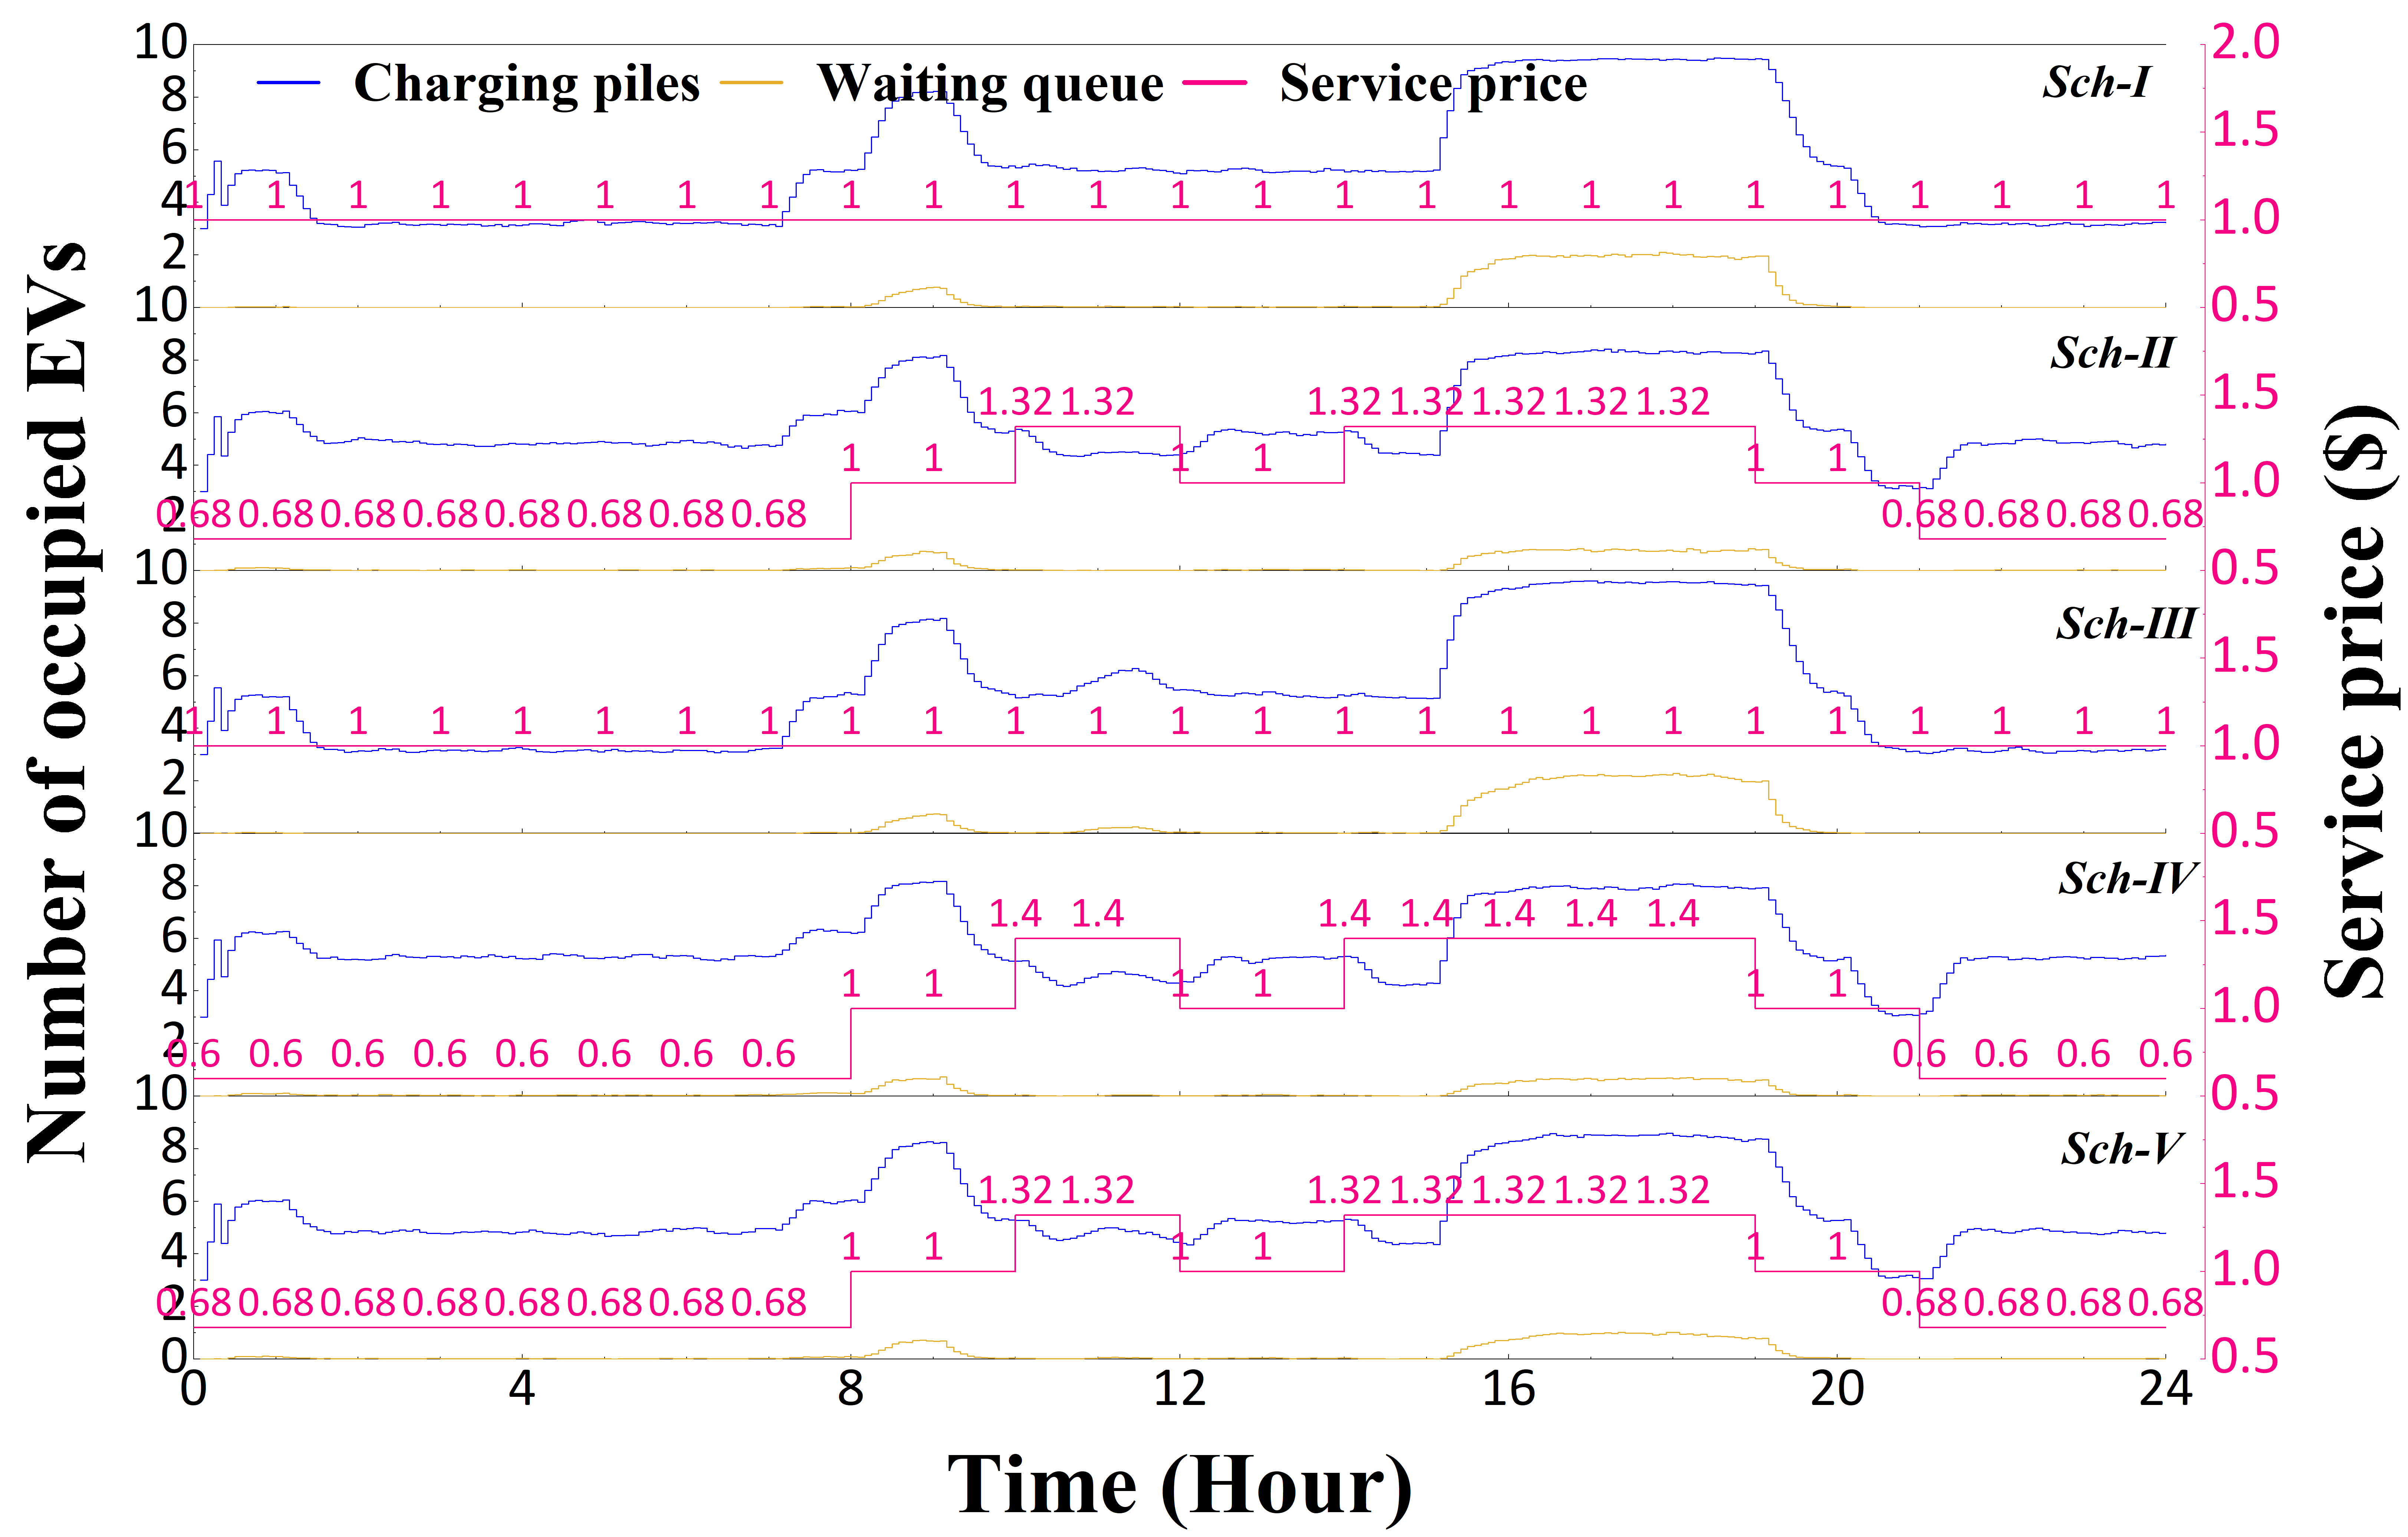
\includegraphics[width=0.98\linewidth]{figures/price_occupy}
\par\end{centering}
\caption{Service Prices, Charging Station Occupancy, and Waiting Queue Length Released by Charging Station under Five Schemes}
\label{fig:Service-Prices,-Charging}
\end{figure}

\begin{table}[tbp]
\caption{Statistical revenues of the five schemes}
\label{tab:Statistical-revenues-of-Five-sch}
\centering{}%
\begin{tabular}{>{\raggedright}p{0.10\columnwidth}>{\raggedleft}p{0.27\columnwidth}>{\raggedleft}p{0.23\columnwidth}>{\raggedleft}p{0.30\columnwidth}}
\hline
\multirow{3}{0.10\columnwidth}{\noindent \centering{}Scheme} & \multirow{3}{0.27\columnwidth}{\noindent \raggedleft{}Total cost of user satisfaction} & \multirow{3}{0.23\columnwidth}{\noindent \raggedleft{}Peak shaving benefits (\$)} & \multirow{3}{0.30\columnwidth}{\noindent \raggedleft{}Revenue from Charging Serves (\$)}\tabularnewline
 &  &  & \tabularnewline
 &  &  & \tabularnewline
\hline
\emph{Sch-I} & 0 & 0 & 27634\tabularnewline
\emph{Sch-\mbox{II}} & 0 & 1652 & 28734\tabularnewline
\emph{Sch-\mbox{III}} & 2117 & 589 & 27415\tabularnewline
\emph{Sch-\mbox{IV}} & 1395 & 3454 & 28227\tabularnewline
\emph{Sch-\mbox{V}} & 643 & 2644 & 28608\tabularnewline
\hline
\end{tabular}
\end{table}

\begin{figure}[htbp]
\noindent \begin{centering}
\subfloat[$\phi_{ps}^{1}$]{\noindent \begin{centering}
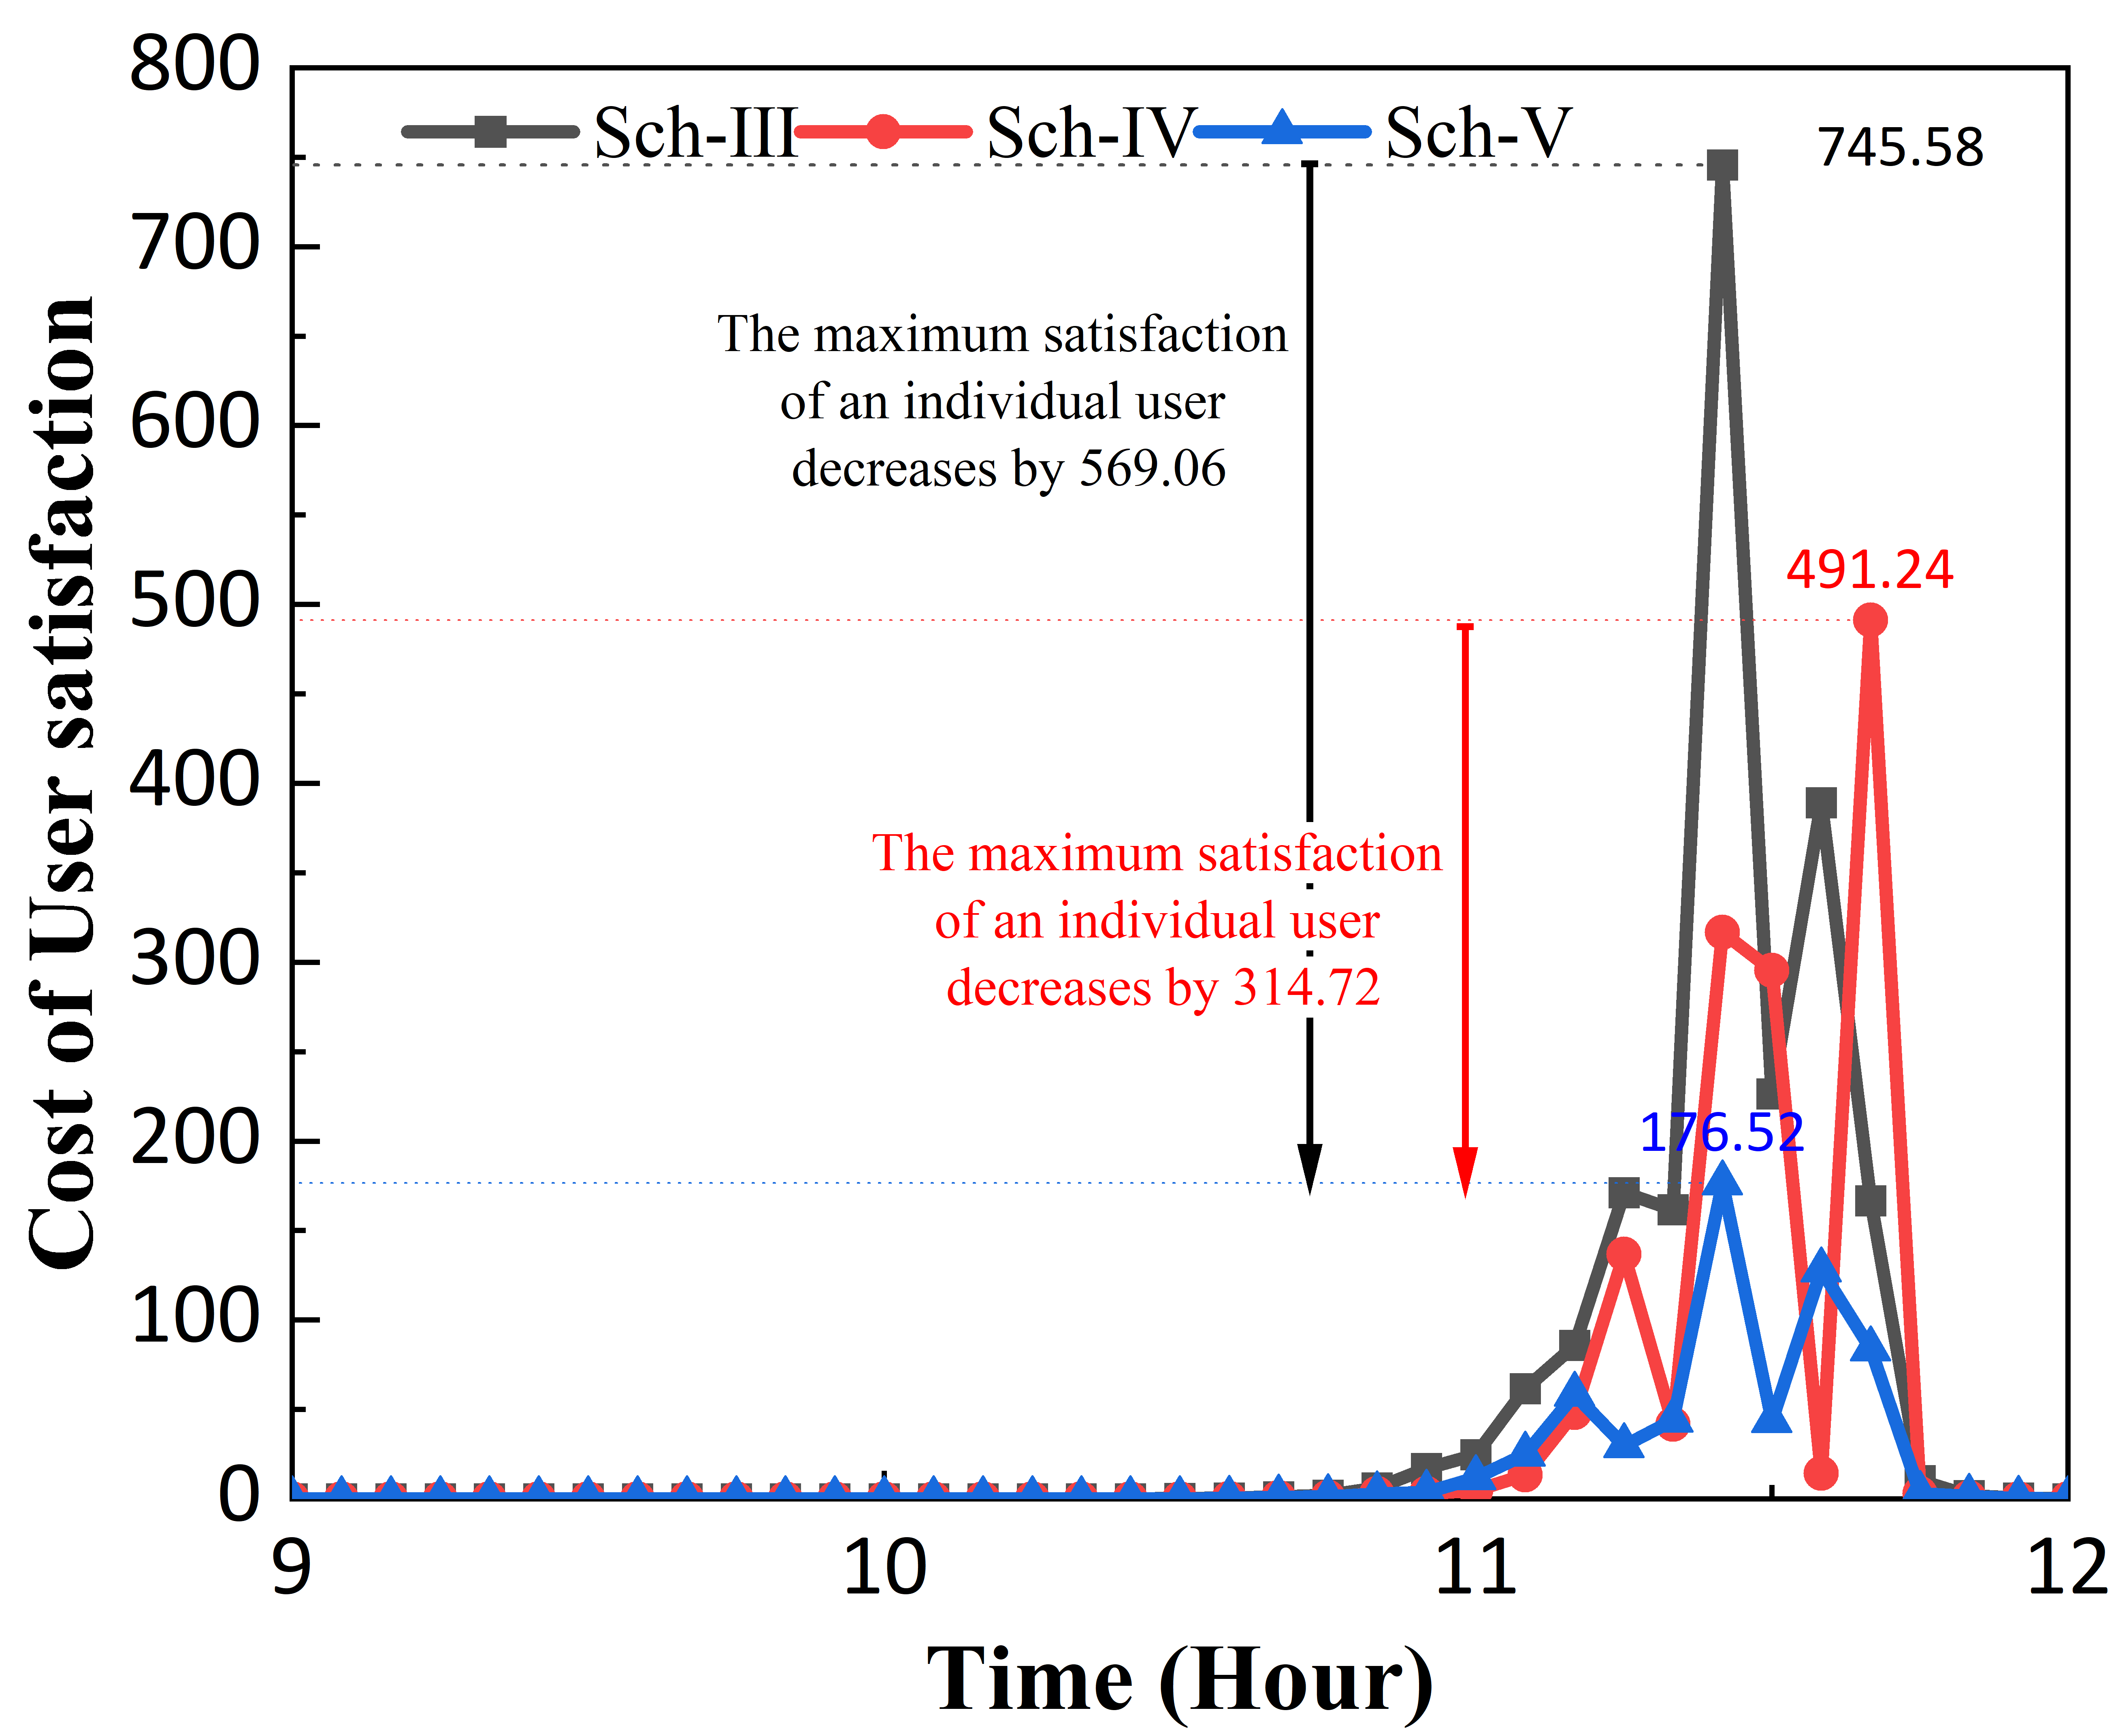
\includegraphics[width=0.49\linewidth]{figures/QoS_peak_period1}
\par\end{centering}
}\subfloat[$\phi_{ps}^{2}$]{\noindent \begin{centering}
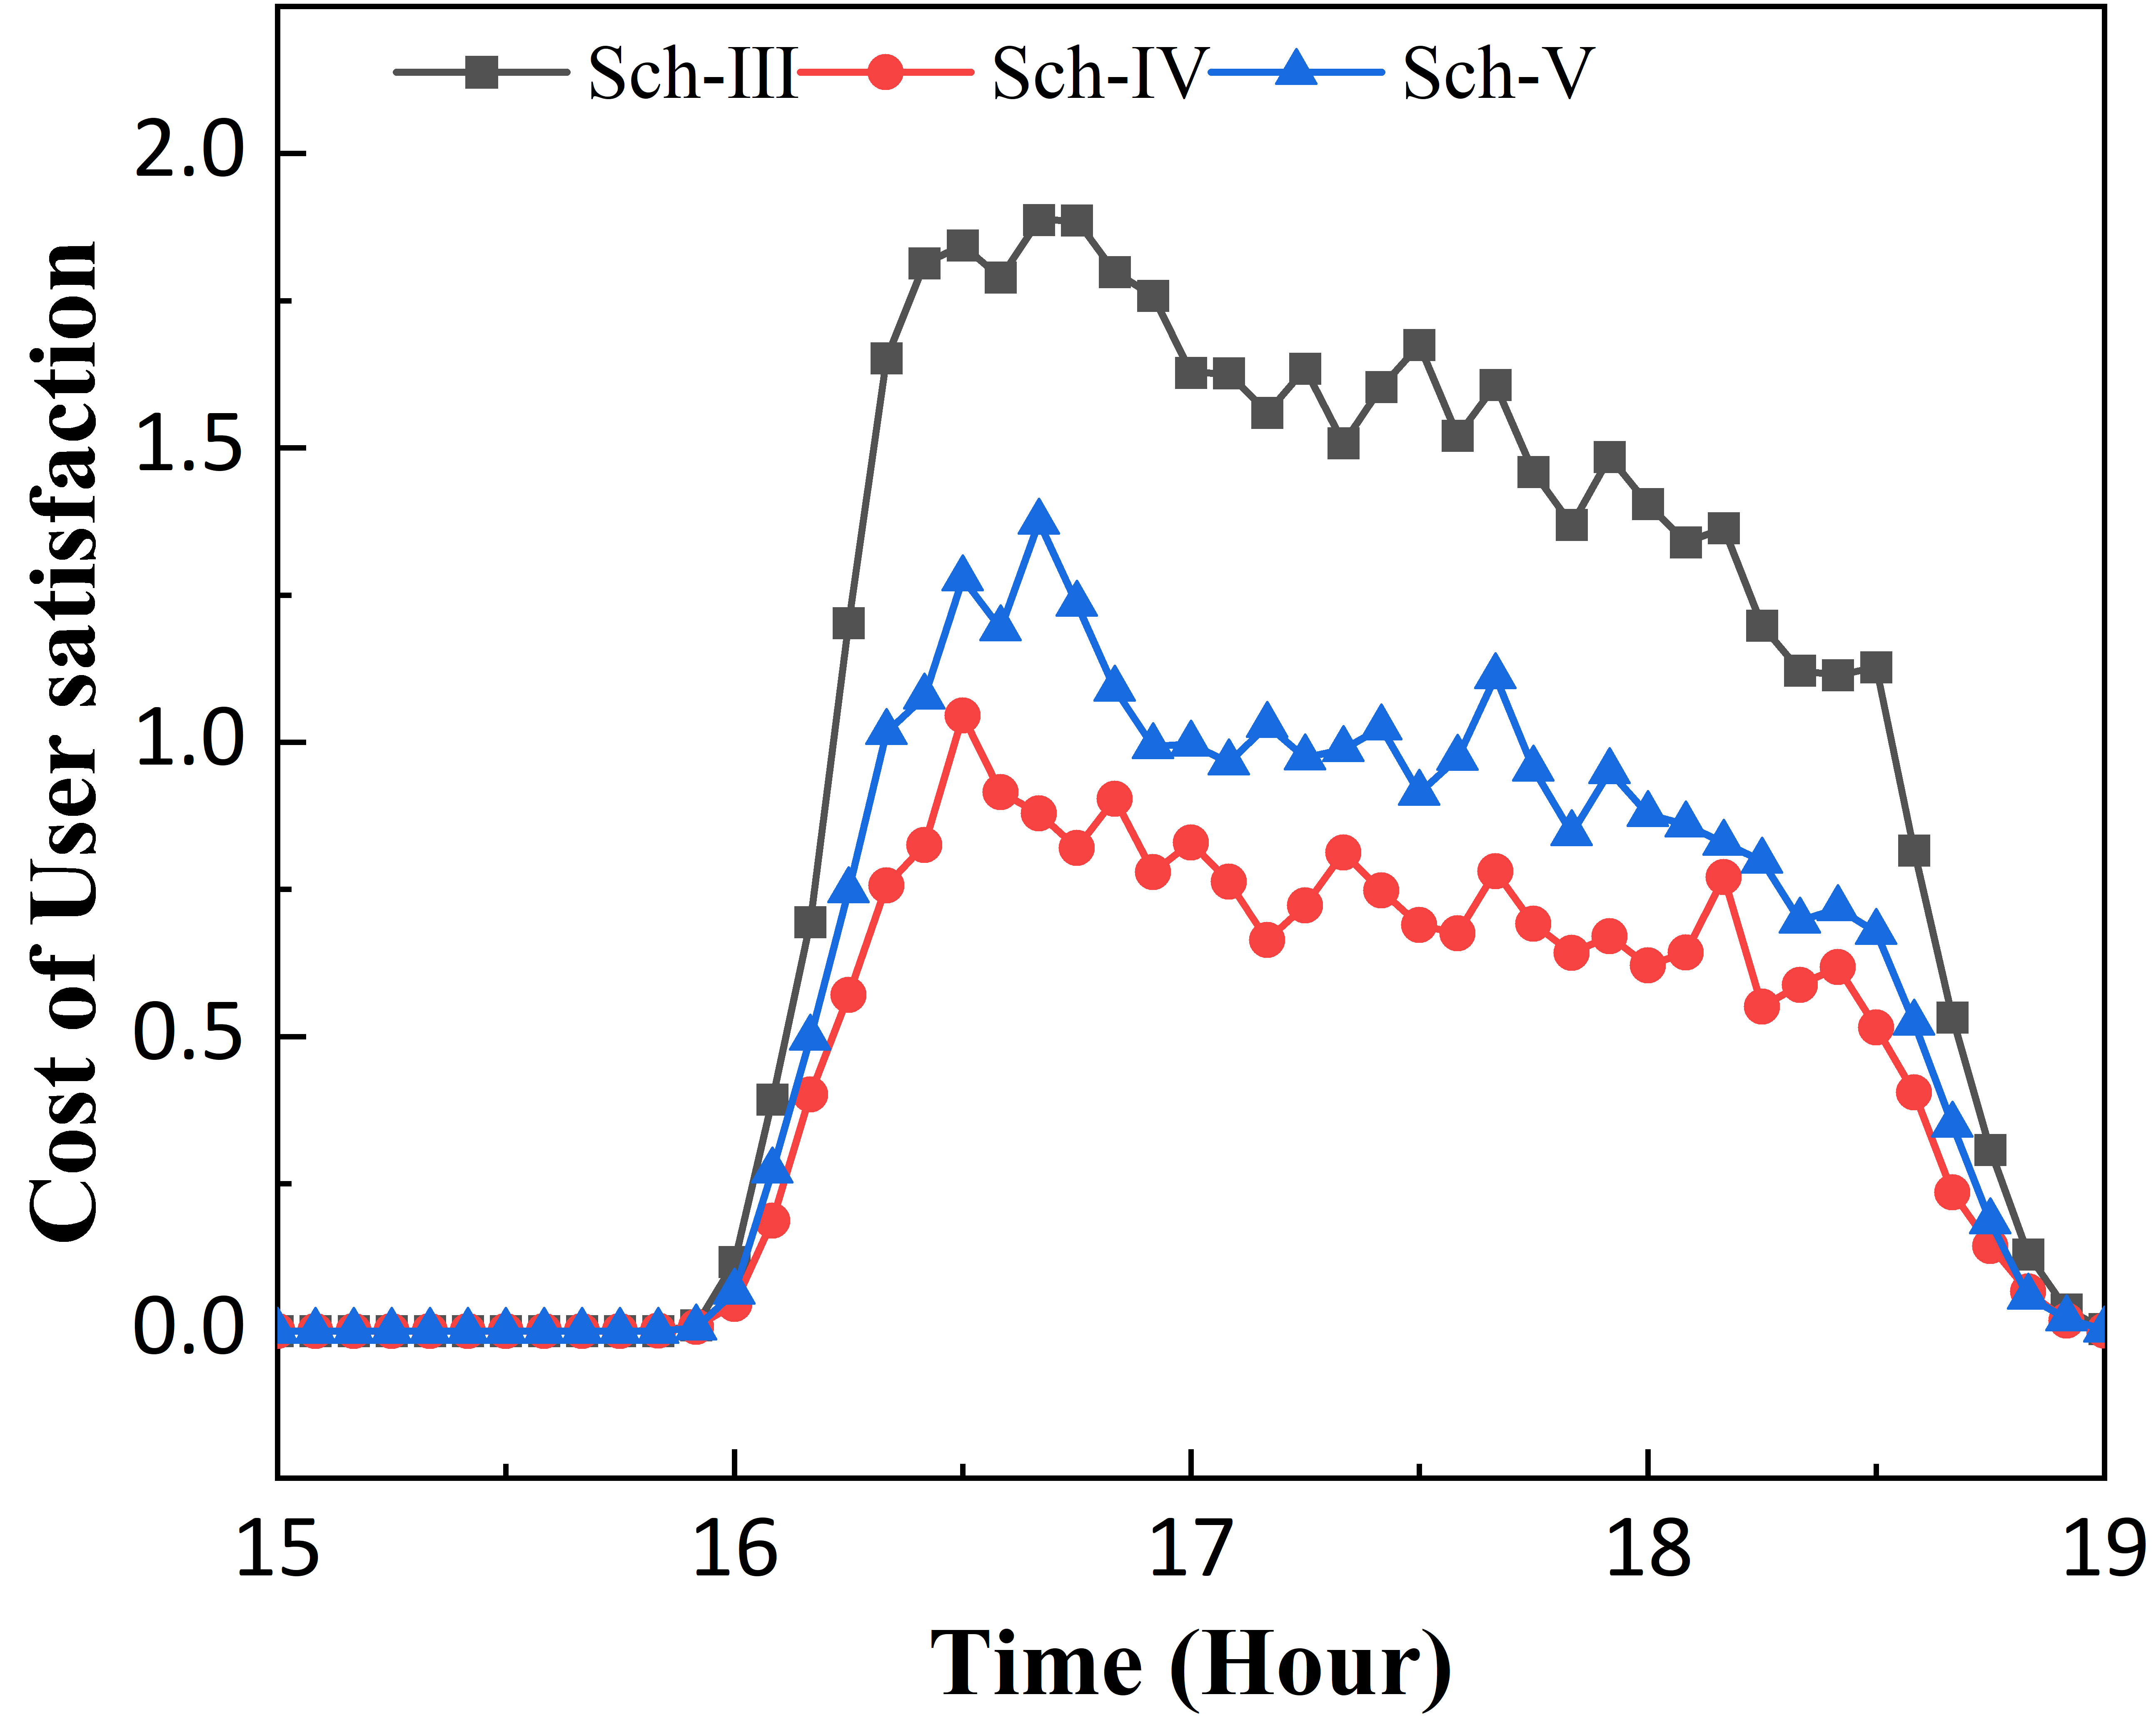
\includegraphics[width=0.49\linewidth]{figures/QoS_peak_period2}
\par\end{centering}
}
\par\end{centering}
\caption{Cost of user satisfaction during the peak-shaving periods}
\label{fig:Cost-of-user}
\end{figure}

To mitigate the high randomness in the simulation data of charging station operations, we conducted simulations for 1000 days using the same random seed under five distinct strategies to draw clearer conclusions.  The mean of various data points was used as the basis for our experimental results. Figure \ref{fig:Charging-Power-Curves3D} presents the power variation curves for 10 charging stations across these five experimental schemes. Notably, \emph{Sch-III} demonstrates limited load adjustment capability, in contrast to \emph{Sch-II}, \emph{IV}, and \emph{V}, which significantly alter station loads. This includes increasing charging load during valley electricity price periods and decreasing consumption during peak periods, largely due to the effective application of price-guided methods in daily load management. Figure \ref{fig:Service-Prices,-Charging} shows that \emph{Sch-II}, \emph{IV}, and \emph{V}, utilizing dynamic service pricing, affect utilization rates and waiting queue lengths at the stations. Specifically, the SPM enhances pile utilization by lowering prices in low-demand periods. During high electricity price periods, increased service prices lead to a marked reduction in both charging pile occupancy and the number of EVs awaiting charging.

% Considering the strong randomness in the simulation data of the charging
% station operation, to ensure clearer conclusions, we simulated the
% operation of the charging station under five different strategies
% with the same random seed for 1000 days. The mean curves of various
% data points are taken as our experimental results. Fig. \ref{fig:Charging-Power-Curves3D}
% illustrates the power variation curves of 10 charging stations under
% five experimental schemes. In comparison to the others, \emph{Sch-\mbox{III}}
% exhibits a significantly limited capacity for load adjustment at the
% station. Conversely, Sch\emph{-\mbox{II}}, \emph{\mbox{IV}}, and \emph{\mbox{V}}
% distinctly modify the station's load, either increasing charging load
% during periods of valley electricity price or decreasing consumption
% during periods of peak electricity price. This is attributed to the
% more pronounced impact of using price-guided methods on the overall
% daily load adjustment of the charging station. As depicted in Fig.
% \ref{fig:Service-Prices,-Charging}, Sch\emph{-\mbox{II}}, \emph{\mbox{IV}},
% and \emph{\mbox{V}}, with the adoption of dynamic service pricing,
% exhibit changes in the utilization rates and waiting queue lengths
% of charging stations. SPM achieves an increase in the utilization
% rate of charging piles by lowering the charging service price during
% periods of low demand. Conversely, during high electricity price periods,
% it raises the service price, resulting in a statistically significant
% reduction in both the occupancy rate of charging piles and the number
% of EVs waiting for charging.

Figure \ref{fig:Charging-Power-Response} demonstrates the peak shaving and valley filling effects of \emph{Sch-II}, \emph{III}, \emph{IV}, and \emph{V}. Each subplot in the upper section of Fig. \ref{fig:Charging-Power-Response} uses a heatmap to compare peak shaving and valley filling for each charging pile against the baseline.  Here, negative values signify valley filling, and positive ones indicate peak shaving.  The area chart in the lower section shows the cumulative power adjustment variations at the station. Obviously, \emph{Sch-III} displays a minimal impact in peak shaving and valley filling.  An analysis of the response of \emph{Sch-II}, \emph{IV}, and \emph{V} during peak periods reveals that \emph{Sch-II} is less responsive, particularly from 16:00 to 19:00, compared to \emph{Sch-IV} and \emph{V}. This reduced effectiveness is due to the limitations of price-based guidance in adjusting charging power within short intervals. Consequently, a control scheme based solely on price guidance proves inadequate for real-time peak shaving requirements of the grid.

% Fig. \ref{fig:Charging-Power-Response} illustrates the peak shaving
% and valley filling effects of Sch\emph{ \mbox{II}},\emph{\mbox{III},
% \mbox{IV}}, and \emph{\mbox{V}}. Each subplot in Fig. \ref{fig:Charging-Power-Response}'s
% upper section employs a heatmap to showcase the peak shaving and valley
% filling for each charging pile compared to the original baseline.
% Negative values indicate valley filling, while positive values indicate
% peak shaving. The lower section's area chart reflects the overall
% power adjustment variations at the station. Obviously, \emph{Sch-\mbox{III}}
% exhibits a very weak effect in terms of peak shaving and valley filling.
% Furthermore, analyzing the response amount of \emph{Sch \mbox{II}},\emph{
% \mbox{IV}, \mbox{IV}} during peak shaving periods, we observe that
% , compared to \emph{Sch \mbox{IV} }and\emph{ \mbox{V}}, \emph{Sch-\mbox{II}}
% shows poor responsiveness, especially during the period from 16:00
% to 19:00. This is attributed to the limited effectiveness of price
% guidance in adjusting charging power over relatively short time periods.
% Therefore, a station control scheme relying solely on price guidance
% is insufficient to meet real-time peak shaving demands of the grid.

A comparison of \emph{Sch-IV} and \emph{V}, as shown in Table \ref{tab:Statistical-revenues-of-Five-sch}, reveals their significant impact on peak shaving and valley filling, including real-time peak shaving.  Notably, \emph{Sch-V} generates higher charging service revenue than \emph{Sch-IV}, indicating the superiority of its trained pricing strategy over \emph{Sch-IV}'s fixed approach. However, \emph{Sch-IV} outperforms \emph{Sch-V} in peak shaving revenue, which can be attributed to two factors. Firstly, \emph{Sch-IV} implements higher service prices during peak periods, as shown in Fig.  \ref{fig:Service-Prices,-Charging}, effectively discouraging user charging and reducing the station's power consumption, thus aligning closely with grid peak shaving directives. Secondly, the CPC strategy in \emph{Sch-V} considers not only peak shaving revenue but also user satisfaction, balancing the cost implications of reducing EV charging power.  As depicted in Fig. \ref{fig:Cost-of-user}, \emph{Sch-V} demonstrates superior user satisfaction performance, particularly during the initial peak shaving period. This outcome underscores the effectiveness of the optimization approach proposed in this study.

% Moreover, comparing \emph{Sch-\mbox{IV}} and \emph{\mbox{V}}, according
% to Table \ref{tab:Statistical-revenues-of-Five-sch}, it can be observed
% that these two schemes exhibit noticeable effects in peak shaving
% and valley filling, as well as real-time peak shaving. Firstly, the
% charging service revenue of \emph{Sch-\mbox{V}} is higher than that
% of \emph{Sch-\mbox{IV}}, indicating that the trained pricing strategy
% in\emph{ Sch-\mbox{V}} is superior to the fixed pricing strategy in
% \emph{Sch-\mbox{IV}}. However, \emph{Sch-\mbox{IV}}'s peak shaving
% revenue is higher than that of \emph{Sch-\mbox{V}}. This could be
% attributed to two reasons. On one hand, \emph{Sch-\mbox{IV}} adopts
% the highest service prices during peak shaving periods, discouraging
% user behavior to the maximum extent and minimizing the station's power
% consumption, making it more responsive to grid peak shaving orders.
% On the other hand, the power allocation strategy of the CPC in \emph{Sch-\mbox{V}}
% not only considers peak shaving revenue but also takes into account
% the user satisfaction cost associated with reducing EV charging power.
% From Fig. \ref{fig:Cost-of-user}, it can be seen that user satisfaction
% performance\emph{ }of \emph{Sch-\mbox{V}} is better than \emph{Sch-\mbox{IV}},
% especially in the first peak shaving period. This validates the effectiveness
% of the optimization method proposed in this paper.


\section{Summary and conclusions}
%%\label{}
In this study, our objective was to optimize the service strategies of EV charging stations, aiming to improve both economic performance and peak demand response. Based on a dynamic electricity pricing and real-time peak shaving mechanism in a specific region, we developed a dual-centralized control scheme with service prices maker and charging power control as adjustment approaches.Addressing the unpredictability of EV user charging behavior and intra-day peak demands, along with the nonlinear costs of user satisfaction, we implemented a data-driven, model-free optimization method. This entailed using the Dueling DQN algorithm for upper-layer service price optimization and the TD3 algorithm for lower-layer power adjustment.
Collaborative signals such as service prices and rewards facilitated the interaction and training of both upper and lower-layer agents within the same simulation environment, culminating in a cohesive strategy. Our simulation results confirmed that the dual-center collaborative approach significantly surpasses the single-center strategy in economic benefits and peak demand response. Furthermore, we introduced an early feature fusion method to refine the decision-making state of the upper-layer agent, enhancing offline training efficiency and post-convergence strategy performance. We contend that this dual-center control scheme and learning optimization approach effectively address the internal economic and external peak demand challenges faced by charging stations. Additionally, this methodology has potential applications for large-scale electricity consumers with adjustment capabilities, such as commercial buildings and industrial power parks. 

However, this research has limitations needing further improvement. The benefits of user participation in demand response are currently based on historical load curves, as dictated by regional policies. This settlement approach might not suit fluctuating loads like those at charging stations, and a rated power-based settlement may be more appropriate.  The paper oversimplifies EV user responses to charging station price changes, assuming immediate behavioral adjustments. Future studies could incorporate a delay element to more realistically model user price response. Moreover, exploring efficient multi-agent optimization methods for collaborative operations across multiple stations remains an essential area for future research.

% The upper-layer service price optimization used the Dueling DQN algorithm, and the lower-layer power adjustment adopted the TD3 algorithm. The service prices and reward serve as collaborative signals, enabling interaction and training of upper and lower-layer agents in the same simulation environment, resulting in a well-coordinated strategy. In simulation examples, we validated that the dual-center collaborative approach significantly outperforms the single-center approach in terms of economic benefits and peak demand response. Additionally, we introduced a early feature fusion method, transforming the decision state of the upper-layer agent, improving offline training time, and post-convergence strategy performance. We believe that the proposed dual-center control scheme and learning optimization can effectively address the internal economic performance and external peak demand response issues of charging stations. And the extending study is also applicable to large-scale electricity users on the demand side with certain adjustment capabilities, such as commercial buildings, industrial power parks, and more. 

% However, there have some drawbacks in this research that require further refinement. Due to the constraints of actual regional policies, the benefits of user participation in demand response are settled based on historical load curves. However, this settlement method may not be suitable for loads with frequent fluctuations like charging stations, and settling based on rated power may be more reliable. The process of EV users responding to the service prices of charging stations is simplified in this paper, assuming that users charging behavior changes immediately after the service prices are issued. In future research, a certain time delay element can be introduced to model the charging users response behavior to prices more accurately. Additionally, employing more efficient multi-agent optimization methods to address collaborative operations among multiple stations is a key focus for future research.

\section*{Acknowledgements}
This work was supported by Natural Science Foundation of China 62273130, Anhui Energy Internet Fund Key Project 2108085UD01 and the funds from China Scholarship Council under Grant 202306690081.
% This work was supported by Natural Science Foundation of China "Modeling and learning optimization methods for the service-oriented power dispatch under random and flexible environment" (62273130), Anhui Energy Internet Fund Key Project "Research on Provincial Power Grid Frequency Coordinated Control Methods Considering Large-Scale Distributed Resources" (JZ2022AKZR0725) and the funds from China Scholarship Council under Grant (202306690081).

%% The Appendices part is started with the command \appendix;
%% appendix sections are then done as normal sections
%% \appendix

%% \section{}
%% \label{}

%% For citations use: 
%%       \citet{<label>} ==> Jones et al. [21]
%%       \citep{<label>} ==> [21]
%%

%% If you have bibdatabase file and want bibtex to generate the
%% bibitems, please use
%%
\bibliographystyle{elsarticle-num-names} 
\bibliography{ref}
\appendix

\section{The Feature Fusion Process of FF1}
%% \label{}
From Eq. \ref{eq:up_decision_state}, the original upper-layer decision
state is

\[
s_{\textrm{up}}^{k}=\left\{ k,p_{\textrm{bl}}^{k},pr_{\textrm{ele}}^{k},B_{\textrm{ps}}^{k},\bar{H}_{c}^{k},\bar{E}_{c}^{k},\bar{\mathbb{P}}_{c}^{k},\bar{p}_{c}^{k},\bar{H}_{w}^{k},\bar{E}_{w}^{k},\bar{\mathbb{P}}_{w}^{k}\right\}
\]

Based on the SoC vector $\bar{H}_{c}^{k}$, the maximum battery capacity
vector $\bar{E}_{c}^{k}$ and the real-time charging power vector
$\bar{p}_{c}^{k}$ of the charging piles, we can infer the remaing
charging time required for each charging pile $\varGamma_{c}^{k}$
as shown in Eq. \ref{eq:cp_remain_charging_time}. Then, we arrange
the remaining charging time vector $\varGamma_{c}^{k}$ in descending
order, resulting in a new state vector denoted as $\overrightarrow{\varGamma}_{c}^{k}$.

Similarly, based on the SoC vector $\bar{H}_{w}^{k}$, maximum battery
capacity vector $\bar{E}_{w}^{k}$, and rated charging power vector
$\bar{\mathbb{P}}_{w}^{k}$ of the waiting queue, we calculate the
estimated charging time for EVs in the queue, denoted as $\varGamma_{w}^{k}$.
Then, we arrange vector $\varGamma_{w}^{k}$ in descending order to
obtain a new state vector, denoted as $\overrightarrow{\varGamma}_{w}^{k}$.

Combining with Formula 1, we obtain the overall load value of the
station, which in turn gives us the fused state of FF1, as shown below

\[
\widetilde{s}_{\textrm{up}}^{k}=\left\{ k,p_{\textrm{bl}}^{k},pr_{\textrm{ele}}^{k},B_{\textrm{ps}}^{k},P_{\textrm{total}}^{k},\overrightarrow{\varGamma}_{c}^{k},\overrightarrow{\varGamma}_{w}^{k}\right\} .
\]


%% else use the following coding to input the bibitems directly in the
%% TeX file.

% \begin{thebibliography}{00}

%% \bibitem[Author(year)]{label}
%% Text of bibliographic item

% \bibitem[ ()]{}

% \end{thebibliography}
\end{document}

\endinput
%%
%% End of file `elsarticle-template-num-names.tex'.
